\documentclass[twoside]{book}

% Packages required by doxygen
\usepackage{fixltx2e}
\usepackage{calc}
\usepackage{doxygen}
\usepackage[export]{adjustbox} % also loads graphicx
\usepackage{graphicx}
\usepackage[utf8]{inputenc}
\usepackage{makeidx}
\usepackage{multicol}
\usepackage{multirow}
\PassOptionsToPackage{warn}{textcomp}
\usepackage{textcomp}
\usepackage[nointegrals]{wasysym}
\usepackage[table]{xcolor}

% Font selection
\usepackage[T1]{fontenc}
\usepackage[scaled=.90]{helvet}
\usepackage{courier}
\usepackage{amssymb}
\usepackage{sectsty}
\renewcommand{\familydefault}{\sfdefault}
\allsectionsfont{%
  \fontseries{bc}\selectfont%
  \color{darkgray}%
}
\renewcommand{\DoxyLabelFont}{%
  \fontseries{bc}\selectfont%
  \color{darkgray}%
}
\newcommand{\+}{\discretionary{\mbox{\scriptsize$\hookleftarrow$}}{}{}}

% Page & text layout
\usepackage{geometry}
\geometry{%
  a4paper,%
  top=2.5cm,%
  bottom=2.5cm,%
  left=2.5cm,%
  right=2.5cm%
}
\tolerance=750
\hfuzz=15pt
\hbadness=750
\setlength{\emergencystretch}{15pt}
\setlength{\parindent}{0cm}
\setlength{\parskip}{3ex plus 2ex minus 2ex}
\makeatletter
\renewcommand{\paragraph}{%
  \@startsection{paragraph}{4}{0ex}{-1.0ex}{1.0ex}{%
    \normalfont\normalsize\bfseries\SS@parafont%
  }%
}
\renewcommand{\subparagraph}{%
  \@startsection{subparagraph}{5}{0ex}{-1.0ex}{1.0ex}{%
    \normalfont\normalsize\bfseries\SS@subparafont%
  }%
}
\makeatother

% Headers & footers
\usepackage{fancyhdr}
\pagestyle{fancyplain}
\fancyhead[LE]{\fancyplain{}{\bfseries\thepage}}
\fancyhead[CE]{\fancyplain{}{}}
\fancyhead[RE]{\fancyplain{}{\bfseries\leftmark}}
\fancyhead[LO]{\fancyplain{}{\bfseries\rightmark}}
\fancyhead[CO]{\fancyplain{}{}}
\fancyhead[RO]{\fancyplain{}{\bfseries\thepage}}
\fancyfoot[LE]{\fancyplain{}{}}
\fancyfoot[CE]{\fancyplain{}{}}
\fancyfoot[RE]{\fancyplain{}{\bfseries\scriptsize Generated by Doxygen }}
\fancyfoot[LO]{\fancyplain{}{\bfseries\scriptsize Generated by Doxygen }}
\fancyfoot[CO]{\fancyplain{}{}}
\fancyfoot[RO]{\fancyplain{}{}}
\renewcommand{\footrulewidth}{0.4pt}
\renewcommand{\chaptermark}[1]{%
  \markboth{#1}{}%
}
\renewcommand{\sectionmark}[1]{%
  \markright{\thesection\ #1}%
}

% Indices & bibliography
\usepackage{natbib}
\usepackage[titles]{tocloft}
\setcounter{tocdepth}{3}
\setcounter{secnumdepth}{5}
\makeindex

% Hyperlinks (required, but should be loaded last)
\usepackage{ifpdf}
\ifpdf
  \usepackage[pdftex,pagebackref=true]{hyperref}
\else
  \usepackage[ps2pdf,pagebackref=true]{hyperref}
\fi
\hypersetup{%
  colorlinks=true,%
  linkcolor=blue,%
  citecolor=blue,%
  unicode%
}

% Custom commands
\newcommand{\clearemptydoublepage}{%
  \newpage{\pagestyle{empty}\cleardoublepage}%
}

\usepackage{caption}
\captionsetup{labelsep=space,justification=centering,font={bf},singlelinecheck=off,skip=4pt,position=top}

%===== C O N T E N T S =====

\begin{document}

% Titlepage & ToC
\hypersetup{pageanchor=false,
             bookmarksnumbered=true,
             pdfencoding=unicode
            }
\pagenumbering{alph}
\begin{titlepage}
\vspace*{7cm}
\begin{center}%
{\Large T\+T\+K4155\+: Embedded and Industrial Computer Systems Design }\\
\vspace*{1cm}
{\large Generated by Doxygen 1.8.13}\\
\end{center}
\end{titlepage}
\clearemptydoublepage
\pagenumbering{roman}
\tableofcontents
\clearemptydoublepage
\pagenumbering{arabic}
\hypersetup{pageanchor=true}

%--- Begin generated contents ---
\chapter{Data Structure Index}
\section{Data Structures}
Here are the data structures with brief descriptions\+:\begin{DoxyCompactList}
\item\contentsline{section}{\hyperlink{structBUTTONS}{B\+U\+T\+T\+O\+NS} \\*Data structure to be used to represent the status of the three buttons }{\pageref{structBUTTONS}}{}
\item\contentsline{section}{\hyperlink{structcan__message__t}{can\+\_\+message\+\_\+t} \\*Struct for C\+AN messages }{\pageref{structcan__message__t}}{}
\item\contentsline{section}{\hyperlink{structJOYSTICK__POS}{J\+O\+Y\+S\+T\+I\+C\+K\+\_\+\+P\+OS} \\*Data structure to be used to represent the joystick position }{\pageref{structJOYSTICK__POS}}{}
\item\contentsline{section}{\hyperlink{structmenu}{menu} \\*Data structure to represent a menu. Points to the text display of the menu, and menus above and below in the structure. Also points to an array of functions to be called when the option is selected }{\pageref{structmenu}}{}
\item\contentsline{section}{\hyperlink{structPID__DATA}{P\+I\+D\+\_\+\+D\+A\+TA} \\*Data structure to be used to represent the P\+I-\/regulator parameters }{\pageref{structPID__DATA}}{}
\item\contentsline{section}{\hyperlink{structSLIDER__POS}{S\+L\+I\+D\+E\+R\+\_\+\+P\+OS} \\*Data structure to be used to represent the position of the two sliders }{\pageref{structSLIDER__POS}}{}
\end{DoxyCompactList}

\chapter{File Index}
\section{File List}
Here is a list of all documented files with brief descriptions\+:\begin{DoxyCompactList}
\item\contentsline{section}{common/\hyperlink{can_8h}{can.\+h} \\*C\+AN struct and enumeration common for node 1 and 2 }{\pageref{can_8h}}{}
\item\contentsline{section}{common/\hyperlink{controller__select_8h}{controller\+\_\+select.\+h} \\*Enumeration for controller selection common for node 1 and 2 }{\pageref{controller__select_8h}}{}
\item\contentsline{section}{common/\hyperlink{difficulty__select_8h}{difficulty\+\_\+select.\+h} \\*Enumeration for difficulty selection common for node 1 and 2 }{\pageref{difficulty__select_8h}}{}
\item\contentsline{section}{common/\hyperlink{fsm__state_8h}{fsm\+\_\+state.\+h} \\*Enumeration for F\+SM states common for node 1 and 2 }{\pageref{fsm__state_8h}}{}
\item\contentsline{section}{common/\hyperlink{songs_8h}{songs.\+h} \\*Enumeration for song selection common for node 1 and 2 }{\pageref{songs_8h}}{}
\item\contentsline{section}{common/\hyperlink{common_2user__input_8h}{user\+\_\+input.\+h} \\*User input constants common for node 1 and 2 }{\pageref{common_2user__input_8h}}{}
\item\contentsline{section}{node1/{\bfseries adc.\+c} }{\pageref{node1_2adc_8c}}{}
\item\contentsline{section}{node1/\hyperlink{node1_2adc_8h}{adc.\+h} \\*Module for converting analog input signals to digital signals }{\pageref{node1_2adc_8h}}{}
\item\contentsline{section}{node1/{\bfseries can\+\_\+driver.\+c} }{\pageref{can__driver_8c}}{}
\item\contentsline{section}{node1/\hyperlink{can__driver_8h}{can\+\_\+driver.\+h} \\*Module for sending and receiving data over the C\+AN bus }{\pageref{can__driver_8h}}{}
\item\contentsline{section}{node1/{\bfseries eeprom\+\_\+driver.\+c} }{\pageref{eeprom__driver_8c}}{}
\item\contentsline{section}{node1/\hyperlink{eeprom__driver_8h}{eeprom\+\_\+driver.\+h} \\*Module for reading from and writing to the E\+E\+P\+R\+OM of the A\+T\+Mega162 }{\pageref{eeprom__driver_8h}}{}
\item\contentsline{section}{node1/{\bfseries fonts.\+c} }{\pageref{fonts_8c}}{}
\item\contentsline{section}{node1/\hyperlink{fonts_8h}{fonts.\+h} \\*Module with font for printing to the O\+L\+ED screen }{\pageref{fonts_8h}}{}
\item\contentsline{section}{node1/{\bfseries fsm.\+c} }{\pageref{node1_2fsm_8c}}{}
\item\contentsline{section}{node1/\hyperlink{node1_2fsm_8h}{fsm.\+h} \\*Module for running the system as a Finite State Machine }{\pageref{node1_2fsm_8h}}{}
\item\contentsline{section}{node1/{\bfseries highscore.\+c} }{\pageref{highscore_8c}}{}
\item\contentsline{section}{node1/\hyperlink{highscore_8h}{highscore.\+h} \\*Module for saving and updating highscores in the non-\/volatile E\+E\+P\+R\+OM }{\pageref{highscore_8h}}{}
\item\contentsline{section}{node1/\hyperlink{node1_2main_8c}{main.\+c} \\*Main program of node 1 }{\pageref{node1_2main_8c}}{}
\item\contentsline{section}{node1/{\bfseries mcp2515\+\_\+driver.\+c} }{\pageref{mcp2515__driver_8c}}{}
\item\contentsline{section}{node1/\hyperlink{mcp2515__driver_8h}{mcp2515\+\_\+driver.\+h} \\*Module for controlling the sending and receiving data over the C\+AN bus }{\pageref{mcp2515__driver_8h}}{}
\item\contentsline{section}{node1/{\bfseries menu.\+c} }{\pageref{menu_8c}}{}
\item\contentsline{section}{node1/\hyperlink{menu_8h}{menu.\+h} \\*Module for the menu system }{\pageref{menu_8h}}{}
\item\contentsline{section}{node1/{\bfseries menu\+\_\+action\+\_\+functions.\+c} }{\pageref{menu__action__functions_8c}}{}
\item\contentsline{section}{node1/\hyperlink{menu__action__functions_8h}{menu\+\_\+action\+\_\+functions.\+h} \\*Module with action functions to be called in the menu system }{\pageref{menu__action__functions_8h}}{}
\item\contentsline{section}{node1/{\bfseries oled.\+c} }{\pageref{oled_8c}}{}
\item\contentsline{section}{node1/\hyperlink{oled_8h}{oled.\+h} \\*Module for controlling and printing to the O\+L\+ED screen }{\pageref{oled_8h}}{}
\item\contentsline{section}{node1/{\bfseries spi\+\_\+driver.\+c} }{\pageref{spi__driver_8c}}{}
\item\contentsline{section}{node1/\hyperlink{spi__driver_8h}{spi\+\_\+driver.\+h} \\*Module for sending and receiving messages over the S\+PI bus }{\pageref{spi__driver_8h}}{}
\item\contentsline{section}{node1/{\bfseries sram.\+c} }{\pageref{sram_8c}}{}
\item\contentsline{section}{node1/\hyperlink{sram_8h}{sram.\+h} \\*Module for reading from and writing to the S\+R\+AM }{\pageref{sram_8h}}{}
\item\contentsline{section}{node1/{\bfseries uart.\+c} }{\pageref{uart_8c}}{}
\item\contentsline{section}{node1/\hyperlink{uart_8h}{uart.\+h} \\*Module for sending and receiving messages through the U\+A\+RT }{\pageref{uart_8h}}{}
\item\contentsline{section}{node1/{\bfseries user\+\_\+input.\+c} }{\pageref{user__input_8c}}{}
\item\contentsline{section}{node1/\hyperlink{node1_2user__input_8h}{user\+\_\+input.\+h} \\*Module for reading and transmitting user input data from the U\+SB multifunction board. }{\pageref{node1_2user__input_8h}}{}
\item\contentsline{section}{node2/{\bfseries adc.\+c} }{\pageref{node2_2adc_8c}}{}
\item\contentsline{section}{node2/\hyperlink{node2_2adc_8h}{adc.\+h} \\*Module for adc-\/fuctionality }{\pageref{node2_2adc_8h}}{}
\item\contentsline{section}{node2/{\bfseries dac.\+c} }{\pageref{dac_8c}}{}
\item\contentsline{section}{node2/\hyperlink{dac_8h}{dac.\+h} \\*Module for dac-\/fuctionality }{\pageref{dac_8h}}{}
\item\contentsline{section}{node2/{\bfseries fsm.\+c} }{\pageref{node2_2fsm_8c}}{}
\item\contentsline{section}{node2/\hyperlink{node2_2fsm_8h}{fsm.\+h} \\*Module consisting of state-\/machine-\/functionality }{\pageref{node2_2fsm_8h}}{}
\item\contentsline{section}{node2/{\bfseries game.\+c} }{\pageref{game_8c}}{}
\item\contentsline{section}{node2/\hyperlink{game_8h}{game.\+h} \\*Module for game-\/fuctionality }{\pageref{game_8h}}{}
\item\contentsline{section}{node2/{\bfseries led.\+c} }{\pageref{led_8c}}{}
\item\contentsline{section}{node2/\hyperlink{led_8h}{led.\+h} \\*Module for led-\/fuctionality }{\pageref{led_8h}}{}
\item\contentsline{section}{node2/\hyperlink{node2_2main_8c}{main.\+c} \\*Main program of node 2 }{\pageref{node2_2main_8c}}{}
\item\contentsline{section}{node2/{\bfseries microbit.\+c} }{\pageref{microbit_8c}}{}
\item\contentsline{section}{node2/\hyperlink{microbit_8h}{microbit.\+h} \\*Module for microbit functionality }{\pageref{microbit_8h}}{}
\item\contentsline{section}{node2/{\bfseries motor.\+c} }{\pageref{motor_8c}}{}
\item\contentsline{section}{node2/\hyperlink{motor_8h}{motor.\+h} \\*Module for motor functionality }{\pageref{motor_8h}}{}
\item\contentsline{section}{node2/{\bfseries music\+\_\+driver.\+c} }{\pageref{music__driver_8c}}{}
\item\contentsline{section}{node2/\hyperlink{music__driver_8h}{music\+\_\+driver.\+h} \\*Module for music functionality }{\pageref{music__driver_8h}}{}
\item\contentsline{section}{node2/\hyperlink{music__metadata_8h}{music\+\_\+metadata.\+h} \\*Module for song notes }{\pageref{music__metadata_8h}}{}
\item\contentsline{section}{node2/{\bfseries pid\+\_\+controller.\+c} }{\pageref{pid__controller_8c}}{}
\item\contentsline{section}{node2/\hyperlink{pid__controller_8h}{pid\+\_\+controller.\+h} \\*Module for P\+ID controller functionality }{\pageref{pid__controller_8h}}{}
\item\contentsline{section}{node2/{\bfseries pwm.\+c} }{\pageref{pwm_8c}}{}
\item\contentsline{section}{node2/\hyperlink{pwm_8h}{pwm.\+h} \\*Module for P\+W\+M-\/signal functionality }{\pageref{pwm_8h}}{}
\item\contentsline{section}{node2/{\bfseries servo\+\_\+driver.\+c} }{\pageref{servo__driver_8c}}{}
\item\contentsline{section}{node2/\hyperlink{servo__driver_8h}{servo\+\_\+driver.\+h} \\*Module for servo functionality }{\pageref{servo__driver_8h}}{}
\item\contentsline{section}{node2/{\bfseries solenoid.\+c} }{\pageref{solenoid_8c}}{}
\item\contentsline{section}{node2/\hyperlink{solenoid_8h}{solenoid.\+h} \\*Module for solenoid functionality }{\pageref{solenoid_8h}}{}
\item\contentsline{section}{node2/{\bfseries timer.\+c} }{\pageref{timer_8c}}{}
\item\contentsline{section}{node2/\hyperlink{timer_8h}{timer.\+h} \\*Module for Sys\+Tick timer delay }{\pageref{timer_8h}}{}
\item\contentsline{section}{node2/{\bfseries user\+\_\+input\+\_\+scaling.\+c} }{\pageref{user__input__scaling_8c}}{}
\item\contentsline{section}{node2/\hyperlink{user__input__scaling_8h}{user\+\_\+input\+\_\+scaling.\+h} \\*Module for scaling user inputs }{\pageref{user__input__scaling_8h}}{}
\end{DoxyCompactList}

\chapter{Data Structure Documentation}
\hypertarget{structBUTTONS}{}\section{B\+U\+T\+T\+O\+NS Struct Reference}
\label{structBUTTONS}\index{B\+U\+T\+T\+O\+NS@{B\+U\+T\+T\+O\+NS}}


Data structure to be used to represent the status of the three buttons.  




{\ttfamily \#include $<$user\+\_\+input.\+h$>$}

\subsection*{Data Fields}
\begin{DoxyCompactItemize}
\item 
\mbox{\Hypertarget{structBUTTONS_a63541eabadda76a11d803d7d231b48ff}\label{structBUTTONS_a63541eabadda76a11d803d7d231b48ff}} 
unsigned int {\bfseries left}
\item 
\mbox{\Hypertarget{structBUTTONS_af09a89bfb8bb03916af79d58ef041d74}\label{structBUTTONS_af09a89bfb8bb03916af79d58ef041d74}} 
unsigned int {\bfseries right}
\item 
\mbox{\Hypertarget{structBUTTONS_a03a0e596156613c34a6cffae80853b6d}\label{structBUTTONS_a03a0e596156613c34a6cffae80853b6d}} 
unsigned int {\bfseries joystick}
\end{DoxyCompactItemize}


\subsection{Detailed Description}
Data structure to be used to represent the status of the three buttons. 

Definition at line 50 of file user\+\_\+input.\+h.



The documentation for this struct was generated from the following file\+:\begin{DoxyCompactItemize}
\item 
node1/\hyperlink{node1_2user__input_8h}{user\+\_\+input.\+h}\end{DoxyCompactItemize}

\hypertarget{structcan__message__t}{}\section{can\+\_\+message\+\_\+t Struct Reference}
\label{structcan__message__t}\index{can\+\_\+message\+\_\+t@{can\+\_\+message\+\_\+t}}


Struct for C\+AN messages.  




{\ttfamily \#include $<$can.\+h$>$}

\subsection*{Data Fields}
\begin{DoxyCompactItemize}
\item 
\mbox{\Hypertarget{structcan__message__t_ac5d7e171bc59d6e5ead8957faa1259a6}\label{structcan__message__t_ac5d7e171bc59d6e5ead8957faa1259a6}} 
uint16\+\_\+t {\bfseries id}
\item 
\mbox{\Hypertarget{structcan__message__t_ab3769058723c86113dc6d4d7c8cf2ec0}\label{structcan__message__t_ab3769058723c86113dc6d4d7c8cf2ec0}} 
char {\bfseries data\+\_\+length}
\item 
\mbox{\Hypertarget{structcan__message__t_a519019132ffdcd9fe783b12c4f280c57}\label{structcan__message__t_a519019132ffdcd9fe783b12c4f280c57}} 
char {\bfseries data} \mbox{[}8\mbox{]}
\end{DoxyCompactItemize}


\subsection{Detailed Description}
Struct for C\+AN messages. 

Definition at line 19 of file can.\+h.



The documentation for this struct was generated from the following file\+:\begin{DoxyCompactItemize}
\item 
common/\hyperlink{can_8h}{can.\+h}\end{DoxyCompactItemize}

\hypertarget{structJOYSTICK__POS}{}\section{J\+O\+Y\+S\+T\+I\+C\+K\+\_\+\+P\+OS Struct Reference}
\label{structJOYSTICK__POS}\index{J\+O\+Y\+S\+T\+I\+C\+K\+\_\+\+P\+OS@{J\+O\+Y\+S\+T\+I\+C\+K\+\_\+\+P\+OS}}


Data structure to be used to represent the joystick position.  




{\ttfamily \#include $<$user\+\_\+input.\+h$>$}

\subsection*{Data Fields}
\begin{DoxyCompactItemize}
\item 
\mbox{\Hypertarget{structJOYSTICK__POS_a11a78aa4431dfe01724b41fe715be3b3}\label{structJOYSTICK__POS_a11a78aa4431dfe01724b41fe715be3b3}} 
int {\bfseries x}
\item 
\mbox{\Hypertarget{structJOYSTICK__POS_a3b557ad6569a35299950e78fbe3495b1}\label{structJOYSTICK__POS_a3b557ad6569a35299950e78fbe3495b1}} 
int {\bfseries y}
\end{DoxyCompactItemize}


\subsection{Detailed Description}
Data structure to be used to represent the joystick position. 

Definition at line 17 of file user\+\_\+input.\+h.



The documentation for this struct was generated from the following file\+:\begin{DoxyCompactItemize}
\item 
node1/\hyperlink{node1_2user__input_8h}{user\+\_\+input.\+h}\end{DoxyCompactItemize}

\hypertarget{structmenu}{}\section{menu Struct Reference}
\label{structmenu}\index{menu@{menu}}


Data structure to represent a menu. Points to the text display of the menu, and menus above and below in the structure. Also points to an array of functions to be called when the option is selected.  




{\ttfamily \#include $<$menu.\+h$>$}



Collaboration diagram for menu\+:\nopagebreak
\begin{figure}[H]
\begin{center}
\leavevmode
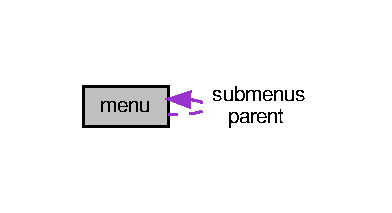
\includegraphics[width=188pt]{structmenu__coll__graph}
\end{center}
\end{figure}
\subsection*{Data Fields}
\begin{DoxyCompactItemize}
\item 
\mbox{\Hypertarget{structmenu_a9cf30093128a1f582de1bdfc1b94c784}\label{structmenu_a9cf30093128a1f582de1bdfc1b94c784}} 
const char $\ast$const  $\ast$ {\bfseries text\+\_\+display}
\item 
\mbox{\Hypertarget{structmenu_ae5f3af0d2cf600f97e3e6011b09cdcf6}\label{structmenu_ae5f3af0d2cf600f97e3e6011b09cdcf6}} 
uint8\+\_\+t {\bfseries length}
\item 
\mbox{\Hypertarget{structmenu_ab37f2faa5398d13b27ca50dcfd4e36e4}\label{structmenu_ab37f2faa5398d13b27ca50dcfd4e36e4}} 
struct \hyperlink{structmenu}{menu} $\ast$ {\bfseries parent}
\item 
\mbox{\Hypertarget{structmenu_a20d5717eb42d807da8fe68a8c0a5eaf6}\label{structmenu_a20d5717eb42d807da8fe68a8c0a5eaf6}} 
struct \hyperlink{structmenu}{menu} $\ast$ {\bfseries submenus} \mbox{[}M\+A\+X\+\_\+\+S\+U\+B\+M\+E\+N\+U\+\_\+\+N\+U\+M\+B\+ER\mbox{]}
\item 
\mbox{\Hypertarget{structmenu_ac32370935be0b516b01cd4cc6d0cf827}\label{structmenu_ac32370935be0b516b01cd4cc6d0cf827}} 
void($\ast$ {\bfseries action\+\_\+functions} \mbox{[}$\,$\mbox{]})()
\end{DoxyCompactItemize}


\subsection{Detailed Description}
Data structure to represent a menu. Points to the text display of the menu, and menus above and below in the structure. Also points to an array of functions to be called when the option is selected. 

Definition at line 22 of file menu.\+h.



The documentation for this struct was generated from the following file\+:\begin{DoxyCompactItemize}
\item 
node1/\hyperlink{menu_8h}{menu.\+h}\end{DoxyCompactItemize}

\hypertarget{structPID__DATA}{}\section{P\+I\+D\+\_\+\+D\+A\+TA Struct Reference}
\label{structPID__DATA}\index{P\+I\+D\+\_\+\+D\+A\+TA@{P\+I\+D\+\_\+\+D\+A\+TA}}


Data structure to be used to represent the P\+I-\/regulator parameters.  




{\ttfamily \#include $<$pid\+\_\+controller.\+h$>$}

\subsection*{Data Fields}
\begin{DoxyCompactItemize}
\item 
\mbox{\Hypertarget{structPID__DATA_aaa1a7edcc47f8fb20a0ed8ce6c50794e}\label{structPID__DATA_aaa1a7edcc47f8fb20a0ed8ce6c50794e}} 
float {\bfseries K\+\_\+p}
\item 
\mbox{\Hypertarget{structPID__DATA_acdea1309ca050514dc9ec0372a48cef5}\label{structPID__DATA_acdea1309ca050514dc9ec0372a48cef5}} 
float {\bfseries K\+\_\+i}
\item 
\mbox{\Hypertarget{structPID__DATA_a34eeea6562e4c200ecbefbc2d6e82c66}\label{structPID__DATA_a34eeea6562e4c200ecbefbc2d6e82c66}} 
float {\bfseries K\+\_\+d}
\item 
\mbox{\Hypertarget{structPID__DATA_a2faf4902ee531d4dd95d52832ce892ea}\label{structPID__DATA_a2faf4902ee531d4dd95d52832ce892ea}} 
int {\bfseries sum\+\_\+error}
\item 
\mbox{\Hypertarget{structPID__DATA_af1a40417fd48fed388ebd241c9efdca9}\label{structPID__DATA_af1a40417fd48fed388ebd241c9efdca9}} 
int {\bfseries prev\+\_\+error}
\item 
\mbox{\Hypertarget{structPID__DATA_ab33028ecd617bcd7b8f5a2b13f7fb6bd}\label{structPID__DATA_ab33028ecd617bcd7b8f5a2b13f7fb6bd}} 
float {\bfseries T}
\item 
\mbox{\Hypertarget{structPID__DATA_a3e809b06f4db55cbe102576b89c19e21}\label{structPID__DATA_a3e809b06f4db55cbe102576b89c19e21}} 
int {\bfseries max\+\_\+u}
\end{DoxyCompactItemize}


\subsection{Detailed Description}
Data structure to be used to represent the P\+I-\/regulator parameters. 

Definition at line 16 of file pid\+\_\+controller.\+h.



The documentation for this struct was generated from the following file\+:\begin{DoxyCompactItemize}
\item 
node2/\hyperlink{pid__controller_8h}{pid\+\_\+controller.\+h}\end{DoxyCompactItemize}

\hypertarget{structSLIDER__POS}{}\section{S\+L\+I\+D\+E\+R\+\_\+\+P\+OS Struct Reference}
\label{structSLIDER__POS}\index{S\+L\+I\+D\+E\+R\+\_\+\+P\+OS@{S\+L\+I\+D\+E\+R\+\_\+\+P\+OS}}


Data structure to be used to represent the position of the two sliders.  




{\ttfamily \#include $<$user\+\_\+input.\+h$>$}

\subsection*{Data Fields}
\begin{DoxyCompactItemize}
\item 
\mbox{\Hypertarget{structSLIDER__POS_a46d181d71ca6dffaf28381563c837a90}\label{structSLIDER__POS_a46d181d71ca6dffaf28381563c837a90}} 
int {\bfseries left}
\item 
\mbox{\Hypertarget{structSLIDER__POS_a1f57530f1fcce456048a7acdbdbf42ab}\label{structSLIDER__POS_a1f57530f1fcce456048a7acdbdbf42ab}} 
int {\bfseries right}
\end{DoxyCompactItemize}


\subsection{Detailed Description}
Data structure to be used to represent the position of the two sliders. 

Definition at line 40 of file user\+\_\+input.\+h.



The documentation for this struct was generated from the following file\+:\begin{DoxyCompactItemize}
\item 
node1/\hyperlink{node1_2user__input_8h}{user\+\_\+input.\+h}\end{DoxyCompactItemize}

\chapter{File Documentation}
\hypertarget{can_8h}{}\section{common/can.h File Reference}
\label{can_8h}\index{common/can.\+h@{common/can.\+h}}


C\+AN struct and enumeration common for node 1 and 2.  


{\ttfamily \#include $<$stdint.\+h$>$}\newline
Include dependency graph for can.\+h\+:
\nopagebreak
\begin{figure}[H]
\begin{center}
\leavevmode
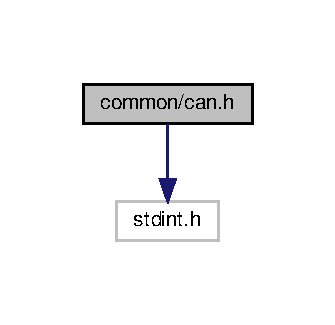
\includegraphics[width=161pt]{can_8h__incl}
\end{center}
\end{figure}
This graph shows which files directly or indirectly include this file\+:
\nopagebreak
\begin{figure}[H]
\begin{center}
\leavevmode
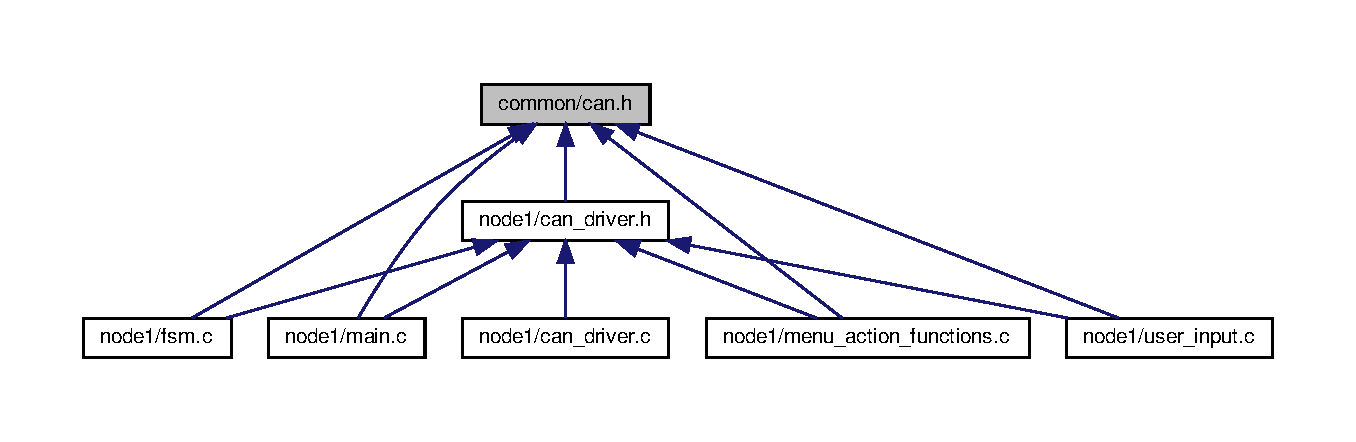
\includegraphics[width=350pt]{can_8h__dep__incl}
\end{center}
\end{figure}
\subsection*{Data Structures}
\begin{DoxyCompactItemize}
\item 
struct \hyperlink{structcan__message__t}{can\+\_\+message\+\_\+t}
\begin{DoxyCompactList}\small\item\em Struct for C\+AN messages. \end{DoxyCompactList}\end{DoxyCompactItemize}
\subsection*{Typedefs}
\begin{DoxyCompactItemize}
\item 
\mbox{\Hypertarget{can_8h_a5918f3dbd6f1aa407afc4f7c34854e08}\label{can_8h_a5918f3dbd6f1aa407afc4f7c34854e08}} 
typedef struct \hyperlink{structcan__message__t}{can\+\_\+message\+\_\+t} \hyperlink{can_8h_a5918f3dbd6f1aa407afc4f7c34854e08}{C\+A\+N\+\_\+\+M\+E\+S\+S\+A\+GE}
\begin{DoxyCompactList}\small\item\em Struct for C\+AN messages. \end{DoxyCompactList}\end{DoxyCompactItemize}
\subsection*{Enumerations}
\begin{DoxyCompactItemize}
\item 
\mbox{\Hypertarget{can_8h_a0db8097ffbefd8c79ce44e8919df462e}\label{can_8h_a0db8097ffbefd8c79ce44e8919df462e}} 
enum \hyperlink{can_8h_a0db8097ffbefd8c79ce44e8919df462e}{C\+A\+N\+\_\+\+M\+E\+S\+S\+A\+G\+E\+\_\+\+ID} \{ \newline
{\bfseries U\+S\+E\+R\+\_\+\+I\+N\+P\+U\+T\+\_\+\+ID} = 1, 
{\bfseries F\+S\+M\+\_\+\+S\+T\+A\+T\+E\+\_\+\+ID}, 
{\bfseries G\+A\+M\+E\+\_\+\+L\+I\+V\+E\+S\+\_\+\+L\+E\+F\+T\+\_\+\+ID}, 
{\bfseries C\+O\+N\+T\+R\+O\+L\+L\+E\+R\+\_\+\+ID}, 
\newline
{\bfseries G\+A\+M\+E\+\_\+\+S\+C\+O\+R\+E\+\_\+\+ID}, 
{\bfseries M\+U\+S\+I\+C\+\_\+\+S\+O\+N\+G\+\_\+\+ID}, 
{\bfseries G\+A\+M\+E\+\_\+\+D\+I\+F\+F\+I\+C\+U\+L\+T\+Y\+\_\+\+ID}
 \}\begin{DoxyCompactList}\small\item\em Enumeration for C\+AN message ID. \end{DoxyCompactList}
\end{DoxyCompactItemize}


\subsection{Detailed Description}
C\+AN struct and enumeration common for node 1 and 2. 


\hypertarget{controller__select_8h}{}\section{common/controller\+\_\+select.h File Reference}
\label{controller__select_8h}\index{common/controller\+\_\+select.\+h@{common/controller\+\_\+select.\+h}}


Enumeration for controller selection common for node 1 and 2.  


This graph shows which files directly or indirectly include this file\+:
\nopagebreak
\begin{figure}[H]
\begin{center}
\leavevmode
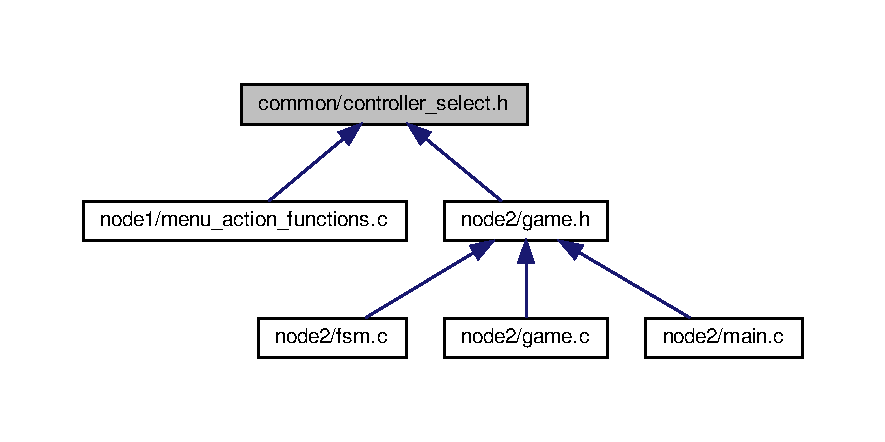
\includegraphics[width=350pt]{controller__select_8h__dep__incl}
\end{center}
\end{figure}
\subsection*{Enumerations}
\begin{DoxyCompactItemize}
\item 
\mbox{\Hypertarget{controller__select_8h_a728b8d7ee2a900a20bf3d786408539aa}\label{controller__select_8h_a728b8d7ee2a900a20bf3d786408539aa}} 
enum {\bfseries C\+O\+N\+T\+R\+O\+L\+L\+E\+R\+\_\+\+S\+EL} \{ {\bfseries S\+L\+I\+D\+E\+R\+\_\+\+P\+O\+S\+\_\+\+C\+T\+RL}, 
{\bfseries J\+O\+Y\+S\+T\+I\+C\+K\+\_\+\+S\+P\+E\+E\+D\+\_\+\+C\+T\+RL}, 
{\bfseries M\+I\+C\+R\+O\+B\+I\+T\+\_\+\+S\+P\+E\+E\+D\+\_\+\+C\+T\+RL}
 \}
\end{DoxyCompactItemize}


\subsection{Detailed Description}
Enumeration for controller selection common for node 1 and 2. 


\hypertarget{difficulty__select_8h}{}\section{common/difficulty\+\_\+select.h File Reference}
\label{difficulty__select_8h}\index{common/difficulty\+\_\+select.\+h@{common/difficulty\+\_\+select.\+h}}


Enumeration for difficulty selection common for node 1 and 2.  


This graph shows which files directly or indirectly include this file\+:
\nopagebreak
\begin{figure}[H]
\begin{center}
\leavevmode
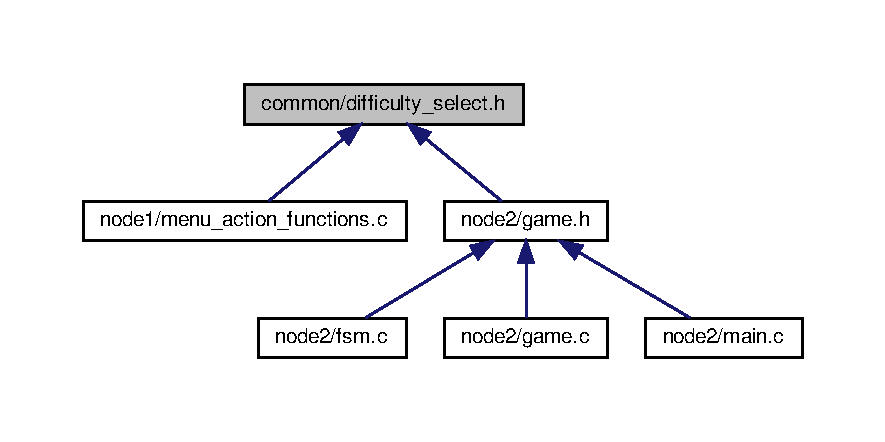
\includegraphics[width=350pt]{difficulty__select_8h__dep__incl}
\end{center}
\end{figure}
\subsection*{Enumerations}
\begin{DoxyCompactItemize}
\item 
\mbox{\Hypertarget{difficulty__select_8h_abad2be49a3ac120910f7f8a1355167a4}\label{difficulty__select_8h_abad2be49a3ac120910f7f8a1355167a4}} 
enum {\bfseries D\+I\+F\+F\+I\+C\+U\+L\+TY} \{ {\bfseries H\+A\+RD}, 
{\bfseries E\+X\+T\+R\+E\+ME}, 
{\bfseries I\+M\+P\+O\+S\+S\+I\+B\+LE}
 \}
\end{DoxyCompactItemize}


\subsection{Detailed Description}
Enumeration for difficulty selection common for node 1 and 2. 


\hypertarget{fsm__state_8h}{}\section{common/fsm\+\_\+state.h File Reference}
\label{fsm__state_8h}\index{common/fsm\+\_\+state.\+h@{common/fsm\+\_\+state.\+h}}


Enumeration for F\+SM states common for node 1 and 2.  


This graph shows which files directly or indirectly include this file\+:
\nopagebreak
\begin{figure}[H]
\begin{center}
\leavevmode
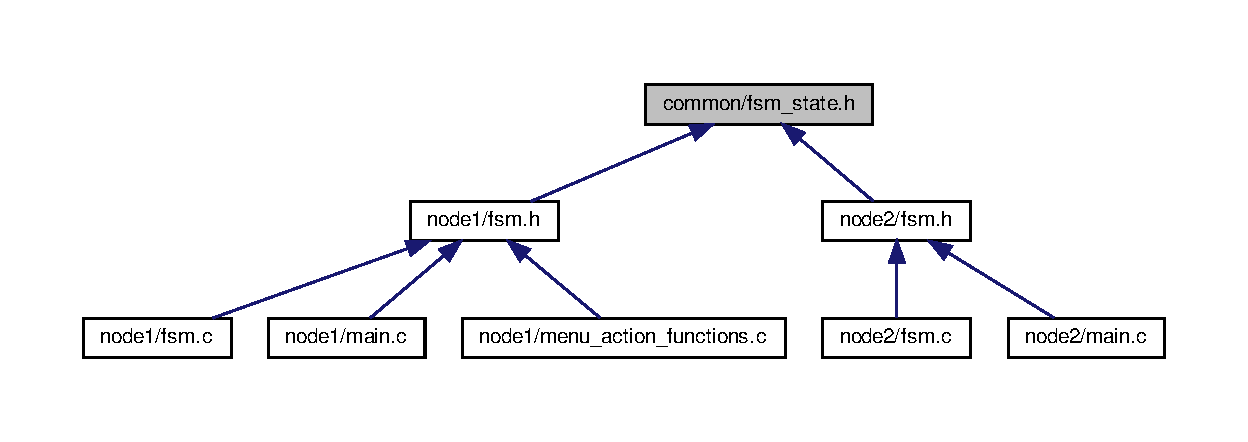
\includegraphics[width=350pt]{fsm__state_8h__dep__incl}
\end{center}
\end{figure}
\subsection*{Enumerations}
\begin{DoxyCompactItemize}
\item 
\mbox{\Hypertarget{fsm__state_8h_afb8cbb8eccb0fea58231b672c43c192f}\label{fsm__state_8h_afb8cbb8eccb0fea58231b672c43c192f}} 
enum {\bfseries F\+S\+M\+\_\+\+S\+T\+A\+TE} \{ \newline
{\bfseries I\+N\+IT}, 
{\bfseries M\+E\+NU}, 
{\bfseries P\+L\+A\+Y\+I\+NG}, 
{\bfseries G\+A\+M\+E\+\_\+\+O\+V\+ER}, 
\newline
{\bfseries I\+D\+LE}
 \}
\end{DoxyCompactItemize}


\subsection{Detailed Description}
Enumeration for F\+SM states common for node 1 and 2. 


\hypertarget{songs_8h}{}\section{common/songs.h File Reference}
\label{songs_8h}\index{common/songs.\+h@{common/songs.\+h}}


Enumeration for song selection common for node 1 and 2.  


This graph shows which files directly or indirectly include this file\+:
\nopagebreak
\begin{figure}[H]
\begin{center}
\leavevmode
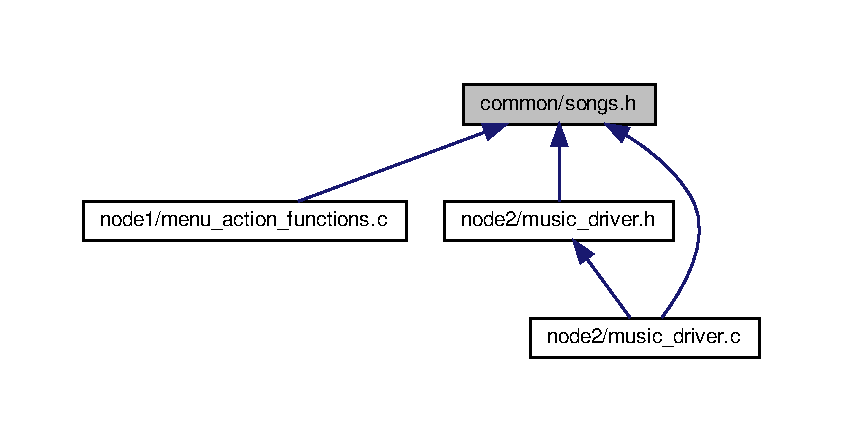
\includegraphics[width=350pt]{songs_8h__dep__incl}
\end{center}
\end{figure}
\subsection*{Enumerations}
\begin{DoxyCompactItemize}
\item 
\mbox{\Hypertarget{songs_8h_ab5ecb3e338a93c686f3716836bceac27}\label{songs_8h_ab5ecb3e338a93c686f3716836bceac27}} 
enum {\bfseries S\+O\+NG} \{ \newline
{\bfseries M\+I\+I\+\_\+\+T\+H\+E\+ME}, 
{\bfseries M\+A\+R\+IO}, 
{\bfseries S\+A\+V\+A\+G\+E\+\_\+\+L\+O\+VE}, 
{\bfseries H\+A\+R\+R\+Y\+\_\+\+P\+O\+T\+T\+ER}, 
\newline
{\bfseries G\+A\+M\+E\+\_\+\+O\+V\+E\+R\+\_\+\+S\+O\+U\+ND}, 
{\bfseries S\+T\+OP}
 \}
\end{DoxyCompactItemize}


\subsection{Detailed Description}
Enumeration for song selection common for node 1 and 2. 


\hypertarget{node1_2adc_8h}{}\section{node1/adc.h File Reference}
\label{node1_2adc_8h}\index{node1/adc.\+h@{node1/adc.\+h}}


Module for converting analog input signals to digital signals.  


{\ttfamily \#include $<$stdint.\+h$>$}\newline
Include dependency graph for adc.\+h\+:\nopagebreak
\begin{figure}[H]
\begin{center}
\leavevmode
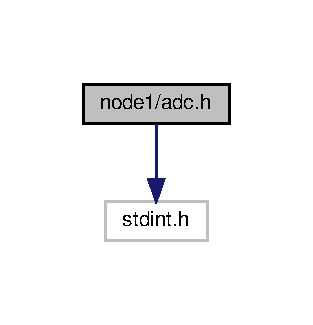
\includegraphics[width=150pt]{node1_2adc_8h__incl}
\end{center}
\end{figure}
This graph shows which files directly or indirectly include this file\+:\nopagebreak
\begin{figure}[H]
\begin{center}
\leavevmode
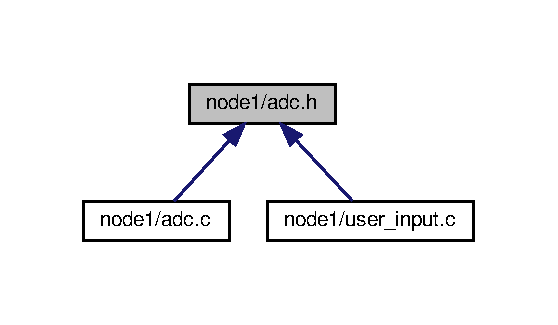
\includegraphics[width=268pt]{node1_2adc_8h__dep__incl}
\end{center}
\end{figure}
\subsection*{Functions}
\begin{DoxyCompactItemize}
\item 
\mbox{\Hypertarget{node1_2adc_8h_ac97938c5997ad9db96f64e94434357ff}\label{node1_2adc_8h_ac97938c5997ad9db96f64e94434357ff}} 
void \hyperlink{node1_2adc_8h_ac97938c5997ad9db96f64e94434357ff}{adc\+\_\+config\+\_\+clock} (void)
\begin{DoxyCompactList}\small\item\em Configurates the external clock signal delivered from the A\+T\+Mega162 to the A\+DC. Sets the frequency to half the frequency of the C\+PU interal clock. \end{DoxyCompactList}\item 
\mbox{\Hypertarget{node1_2adc_8h_a2b815e6730e8723a6d1d06d9ef8f31c0}\label{node1_2adc_8h_a2b815e6730e8723a6d1d06d9ef8f31c0}} 
void \hyperlink{node1_2adc_8h_a2b815e6730e8723a6d1d06d9ef8f31c0}{adc\+\_\+init} (void)
\begin{DoxyCompactList}\small\item\em Initiates the A\+DC by configuring the external clock. \end{DoxyCompactList}\item 
uint8\+\_\+t \hyperlink{node1_2adc_8h_ac1513709a7d29dc6590d9371b8cd0556}{adc\+\_\+read} (uint8\+\_\+t channel)
\begin{DoxyCompactList}\small\item\em Reads the output data from the A\+DC conversion. Starts the conversion by writing to the A\+DC address space, and reads serially until data from channel {\ttfamily channel} is read. \end{DoxyCompactList}\end{DoxyCompactItemize}


\subsection{Detailed Description}
Module for converting analog input signals to digital signals. 



\subsection{Function Documentation}
\mbox{\Hypertarget{node1_2adc_8h_ac1513709a7d29dc6590d9371b8cd0556}\label{node1_2adc_8h_ac1513709a7d29dc6590d9371b8cd0556}} 
\index{node1/adc.\+h@{node1/adc.\+h}!adc\+\_\+read@{adc\+\_\+read}}
\index{adc\+\_\+read@{adc\+\_\+read}!node1/adc.\+h@{node1/adc.\+h}}
\subsubsection{\texorpdfstring{adc\+\_\+read()}{adc\_read()}}
{\footnotesize\ttfamily uint8\+\_\+t adc\+\_\+read (\begin{DoxyParamCaption}\item[{uint8\+\_\+t}]{channel }\end{DoxyParamCaption})}



Reads the output data from the A\+DC conversion. Starts the conversion by writing to the A\+DC address space, and reads serially until data from channel {\ttfamily channel} is read. 


\begin{DoxyParams}{Parameters}
{\em channel} & The analog channel to be read from\\
\hline
\end{DoxyParams}
\begin{DoxyReturn}{Returns}
The output data from the conversion of channel {\ttfamily channel}. 
\end{DoxyReturn}


Definition at line 39 of file adc.\+c.


\hypertarget{node2_2adc_8h}{}\section{node2/adc.h File Reference}
\label{node2_2adc_8h}\index{node2/adc.\+h@{node2/adc.\+h}}


Module for adc-\/fuctionality.  


{\ttfamily \#include $<$stdint.\+h$>$}\newline
Include dependency graph for adc.\+h\+:\nopagebreak
\begin{figure}[H]
\begin{center}
\leavevmode
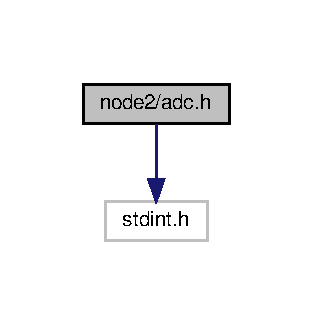
\includegraphics[width=150pt]{node2_2adc_8h__incl}
\end{center}
\end{figure}
This graph shows which files directly or indirectly include this file\+:\nopagebreak
\begin{figure}[H]
\begin{center}
\leavevmode
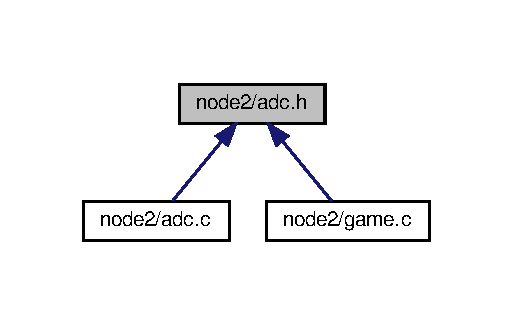
\includegraphics[width=246pt]{node2_2adc_8h__dep__incl}
\end{center}
\end{figure}
\subsection*{Functions}
\begin{DoxyCompactItemize}
\item 
void \hyperlink{node2_2adc_8h_a2b815e6730e8723a6d1d06d9ef8f31c0}{adc\+\_\+init} (void)
\begin{DoxyCompactList}\small\item\em Initiates the A\+DC by setting its mode and clock source, and configuring its P\+MC settings. \end{DoxyCompactList}\item 
uint16\+\_\+t \hyperlink{node2_2adc_8h_a1780a2a12aeb6ba6d00d18c528205159}{adc\+\_\+read} ()
\begin{DoxyCompactList}\small\item\em Reads the A\+DC channel 0. \end{DoxyCompactList}\end{DoxyCompactItemize}


\subsection{Detailed Description}
Module for adc-\/fuctionality. 



\subsection{Function Documentation}
\mbox{\Hypertarget{node2_2adc_8h_a2b815e6730e8723a6d1d06d9ef8f31c0}\label{node2_2adc_8h_a2b815e6730e8723a6d1d06d9ef8f31c0}} 
\index{node2/adc.\+h@{node2/adc.\+h}!adc\+\_\+init@{adc\+\_\+init}}
\index{adc\+\_\+init@{adc\+\_\+init}!node2/adc.\+h@{node2/adc.\+h}}
\subsubsection{\texorpdfstring{adc\+\_\+init()}{adc\_init()}}
{\footnotesize\ttfamily void adc\+\_\+init (\begin{DoxyParamCaption}\item[{void}]{ }\end{DoxyParamCaption})}



Initiates the A\+DC by setting its mode and clock source, and configuring its P\+MC settings. 

Initiates the A\+DC by setting its mode and clock source, and configuring its P\+MC settings. 

Definition at line 34 of file adc.\+c.

\mbox{\Hypertarget{node2_2adc_8h_a1780a2a12aeb6ba6d00d18c528205159}\label{node2_2adc_8h_a1780a2a12aeb6ba6d00d18c528205159}} 
\index{node2/adc.\+h@{node2/adc.\+h}!adc\+\_\+read@{adc\+\_\+read}}
\index{adc\+\_\+read@{adc\+\_\+read}!node2/adc.\+h@{node2/adc.\+h}}
\subsubsection{\texorpdfstring{adc\+\_\+read()}{adc\_read()}}
{\footnotesize\ttfamily uint16\+\_\+t adc\+\_\+read (\begin{DoxyParamCaption}{ }\end{DoxyParamCaption})}



Reads the A\+DC channel 0. 

\begin{DoxyReturn}{Returns}
The converted value at the A\+DC pin, with type {\ttfamily uint16\+\_\+t}. 
\end{DoxyReturn}


Definition at line 25 of file adc.\+c.


\hypertarget{can__driver_8h}{}\section{node1/can\+\_\+driver.h File Reference}
\label{can__driver_8h}\index{node1/can\+\_\+driver.\+h@{node1/can\+\_\+driver.\+h}}


Module for sending and receiving data over the C\+AN bus.  


{\ttfamily \#include \char`\"{}mcp2515\+\_\+driver.\+h\char`\"{}}\newline
{\ttfamily \#include \char`\"{}../common/can.\+h\char`\"{}}\newline
{\ttfamily \#include $<$stdint.\+h$>$}\newline
Include dependency graph for can\+\_\+driver.\+h\+:
\nopagebreak
\begin{figure}[H]
\begin{center}
\leavevmode
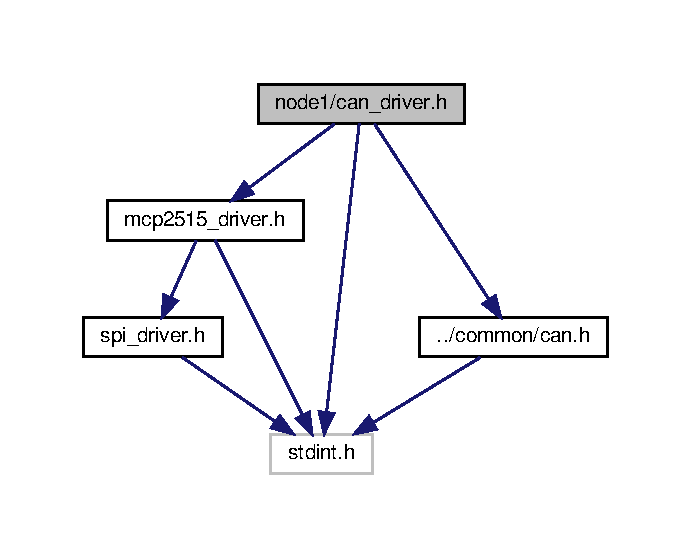
\includegraphics[width=332pt]{can__driver_8h__incl}
\end{center}
\end{figure}
This graph shows which files directly or indirectly include this file\+:\nopagebreak
\begin{figure}[H]
\begin{center}
\leavevmode
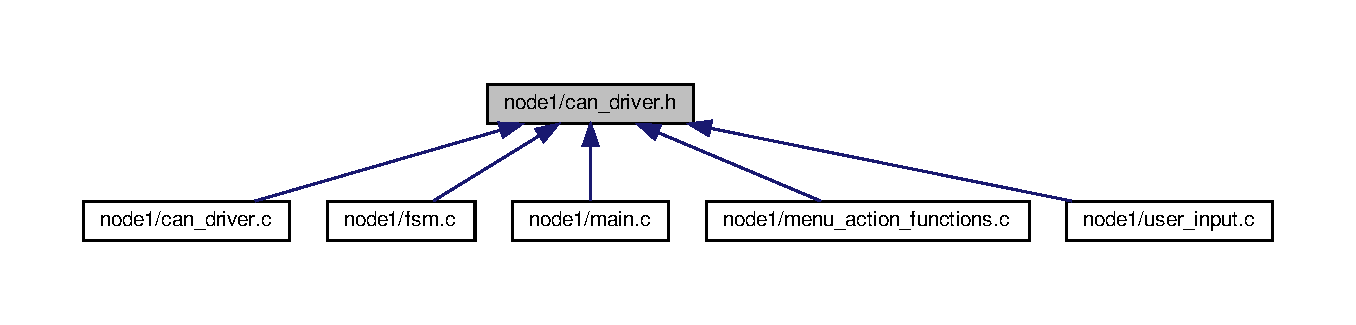
\includegraphics[width=350pt]{can__driver_8h__dep__incl}
\end{center}
\end{figure}
\subsection*{Functions}
\begin{DoxyCompactItemize}
\item 
void \hyperlink{can__driver_8h_a7ee6213bfaeacdb7d26ef64cc213c846}{can\+\_\+init} (uint8\+\_\+t mode)
\begin{DoxyCompactList}\small\item\em Data structure to be used for messages sent using the C\+AN interface. \end{DoxyCompactList}\item 
void \hyperlink{can__driver_8h_a935732faa9f8acfbc2fe7ac9e9001033}{can\+\_\+send} (\hyperlink{can_8h_a5918f3dbd6f1aa407afc4f7c34854e08}{C\+A\+N\+\_\+\+M\+E\+S\+S\+A\+GE} $\ast$message)
\begin{DoxyCompactList}\small\item\em Transmits a message of type {\ttfamily C\+A\+N\+\_\+\+M\+E\+S\+S\+A\+GE} using the C\+AN interface. Uses transmit buffer {\ttfamily T\+X\+B0}. \end{DoxyCompactList}\item 
int \hyperlink{can__driver_8h_a32e14e772cf104ed3251fb44ca098b7c}{can\+\_\+recieve} (\hyperlink{can_8h_a5918f3dbd6f1aa407afc4f7c34854e08}{C\+A\+N\+\_\+\+M\+E\+S\+S\+A\+GE} $\ast$message)
\begin{DoxyCompactList}\small\item\em Recieves a message of type {\ttfamily C\+A\+N\+\_\+\+M\+E\+S\+S\+A\+GE} using the C\+AN interface. Uses recieve buffer {\ttfamily R\+X\+B0} or {\ttfamily R\+B\+X1}, depending on the interrupt flag register of the M\+C\+P2515. \end{DoxyCompactList}\end{DoxyCompactItemize}


\subsection{Detailed Description}
Module for sending and receiving data over the C\+AN bus. 



\subsection{Function Documentation}
\mbox{\Hypertarget{can__driver_8h_a7ee6213bfaeacdb7d26ef64cc213c846}\label{can__driver_8h_a7ee6213bfaeacdb7d26ef64cc213c846}} 
\index{can\+\_\+driver.\+h@{can\+\_\+driver.\+h}!can\+\_\+init@{can\+\_\+init}}
\index{can\+\_\+init@{can\+\_\+init}!can\+\_\+driver.\+h@{can\+\_\+driver.\+h}}
\subsubsection{\texorpdfstring{can\+\_\+init()}{can\_init()}}
{\footnotesize\ttfamily void can\+\_\+init (\begin{DoxyParamCaption}\item[{uint8\+\_\+t}]{mode }\end{DoxyParamCaption})}



Data structure to be used for messages sent using the C\+AN interface. 

Initiates the C\+AN interface, by setting the M\+C\+P2515 to the desired mode, and enabling interrupt on message reception.


\begin{DoxyParams}{Parameters}
{\em mode} & Mode M\+C\+P2515 is being set to. \\
\hline
\end{DoxyParams}


Definition at line 21 of file can\+\_\+driver.\+c.

\mbox{\Hypertarget{can__driver_8h_a32e14e772cf104ed3251fb44ca098b7c}\label{can__driver_8h_a32e14e772cf104ed3251fb44ca098b7c}} 
\index{can\+\_\+driver.\+h@{can\+\_\+driver.\+h}!can\+\_\+recieve@{can\+\_\+recieve}}
\index{can\+\_\+recieve@{can\+\_\+recieve}!can\+\_\+driver.\+h@{can\+\_\+driver.\+h}}
\subsubsection{\texorpdfstring{can\+\_\+recieve()}{can\_recieve()}}
{\footnotesize\ttfamily int can\+\_\+recieve (\begin{DoxyParamCaption}\item[{\hyperlink{can_8h_a5918f3dbd6f1aa407afc4f7c34854e08}{C\+A\+N\+\_\+\+M\+E\+S\+S\+A\+GE} $\ast$}]{message }\end{DoxyParamCaption})}



Recieves a message of type {\ttfamily C\+A\+N\+\_\+\+M\+E\+S\+S\+A\+GE} using the C\+AN interface. Uses recieve buffer {\ttfamily R\+X\+B0} or {\ttfamily R\+B\+X1}, depending on the interrupt flag register of the M\+C\+P2515. 


\begin{DoxyParams}{Parameters}
{\em message} & Pointer to the message being recieved to.\\
\hline
\end{DoxyParams}
\begin{DoxyReturn}{Returns}
0 on success, 1 on failure. 
\end{DoxyReturn}


Definition at line 48 of file can\+\_\+driver.\+c.

\mbox{\Hypertarget{can__driver_8h_a935732faa9f8acfbc2fe7ac9e9001033}\label{can__driver_8h_a935732faa9f8acfbc2fe7ac9e9001033}} 
\index{can\+\_\+driver.\+h@{can\+\_\+driver.\+h}!can\+\_\+send@{can\+\_\+send}}
\index{can\+\_\+send@{can\+\_\+send}!can\+\_\+driver.\+h@{can\+\_\+driver.\+h}}
\subsubsection{\texorpdfstring{can\+\_\+send()}{can\_send()}}
{\footnotesize\ttfamily void can\+\_\+send (\begin{DoxyParamCaption}\item[{\hyperlink{can_8h_a5918f3dbd6f1aa407afc4f7c34854e08}{C\+A\+N\+\_\+\+M\+E\+S\+S\+A\+GE} $\ast$}]{message }\end{DoxyParamCaption})}



Transmits a message of type {\ttfamily C\+A\+N\+\_\+\+M\+E\+S\+S\+A\+GE} using the C\+AN interface. Uses transmit buffer {\ttfamily T\+X\+B0}. 


\begin{DoxyParams}{Parameters}
{\em message} & Pointer to the message being sent. \\
\hline
\end{DoxyParams}


Definition at line 34 of file can\+\_\+driver.\+c.


\hypertarget{eeprom__driver_8h}{}\section{node1/eeprom\+\_\+driver.h File Reference}
\label{eeprom__driver_8h}\index{node1/eeprom\+\_\+driver.\+h@{node1/eeprom\+\_\+driver.\+h}}


Module for reading from and writing to the E\+E\+P\+R\+OM of the A\+T\+Mega162.  


This graph shows which files directly or indirectly include this file\+:\nopagebreak
\begin{figure}[H]
\begin{center}
\leavevmode
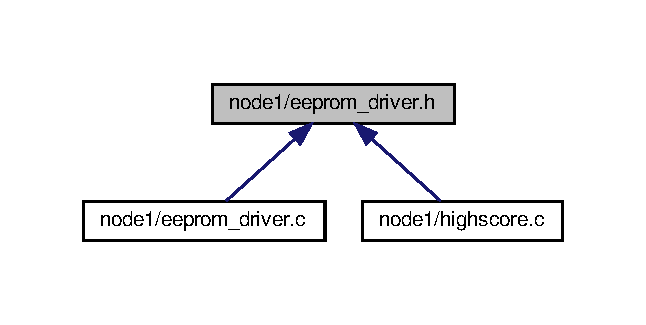
\includegraphics[width=310pt]{eeprom__driver_8h__dep__incl}
\end{center}
\end{figure}
\subsection*{Functions}
\begin{DoxyCompactItemize}
\item 
void \hyperlink{eeprom__driver_8h_a23be9e5de8414d8c781308d2deed169b}{eeprom\+\_\+write} (unsigned int address, unsigned char data)
\begin{DoxyCompactList}\small\item\em Writes {\ttfamily data} to the E\+E\+P\+R\+OM memory address {\ttfamily address}. \end{DoxyCompactList}\item 
unsigned char \hyperlink{eeprom__driver_8h_acb77b6d54f181385535caf60f55114cc}{eeprom\+\_\+read} (unsigned int address)
\begin{DoxyCompactList}\small\item\em Reads a data byte from the E\+E\+P\+R\+OM memory address {\ttfamily address}. \end{DoxyCompactList}\end{DoxyCompactItemize}


\subsection{Detailed Description}
Module for reading from and writing to the E\+E\+P\+R\+OM of the A\+T\+Mega162. 



\subsection{Function Documentation}
\mbox{\Hypertarget{eeprom__driver_8h_acb77b6d54f181385535caf60f55114cc}\label{eeprom__driver_8h_acb77b6d54f181385535caf60f55114cc}} 
\index{eeprom\+\_\+driver.\+h@{eeprom\+\_\+driver.\+h}!eeprom\+\_\+read@{eeprom\+\_\+read}}
\index{eeprom\+\_\+read@{eeprom\+\_\+read}!eeprom\+\_\+driver.\+h@{eeprom\+\_\+driver.\+h}}
\subsubsection{\texorpdfstring{eeprom\+\_\+read()}{eeprom\_read()}}
{\footnotesize\ttfamily unsigned char eeprom\+\_\+read (\begin{DoxyParamCaption}\item[{unsigned int}]{address }\end{DoxyParamCaption})}



Reads a data byte from the E\+E\+P\+R\+OM memory address {\ttfamily address}. 


\begin{DoxyParams}{Parameters}
{\em address} & Memory address to be read from.\\
\hline
\end{DoxyParams}
\begin{DoxyReturn}{Returns}
Data byte at memory address {\ttfamily address}. 
\end{DoxyReturn}


Definition at line 28 of file eeprom\+\_\+driver.\+c.

\mbox{\Hypertarget{eeprom__driver_8h_a23be9e5de8414d8c781308d2deed169b}\label{eeprom__driver_8h_a23be9e5de8414d8c781308d2deed169b}} 
\index{eeprom\+\_\+driver.\+h@{eeprom\+\_\+driver.\+h}!eeprom\+\_\+write@{eeprom\+\_\+write}}
\index{eeprom\+\_\+write@{eeprom\+\_\+write}!eeprom\+\_\+driver.\+h@{eeprom\+\_\+driver.\+h}}
\subsubsection{\texorpdfstring{eeprom\+\_\+write()}{eeprom\_write()}}
{\footnotesize\ttfamily void eeprom\+\_\+write (\begin{DoxyParamCaption}\item[{unsigned int}]{address,  }\item[{unsigned char}]{data }\end{DoxyParamCaption})}



Writes {\ttfamily data} to the E\+E\+P\+R\+OM memory address {\ttfamily address}. 


\begin{DoxyParams}{Parameters}
{\em address} & Memory address to be written to. \\
\hline
{\em data} & Data to be written. \\
\hline
\end{DoxyParams}


Definition at line 6 of file eeprom\+\_\+driver.\+c.


\hypertarget{fonts_8h}{}\section{node1/fonts.h File Reference}
\label{fonts_8h}\index{node1/fonts.\+h@{node1/fonts.\+h}}


Module with font for printing to the O\+L\+ED screen.  


{\ttfamily \#include $<$avr/pgmspace.\+h$>$}\newline
Include dependency graph for fonts.\+h\+:\nopagebreak
\begin{figure}[H]
\begin{center}
\leavevmode
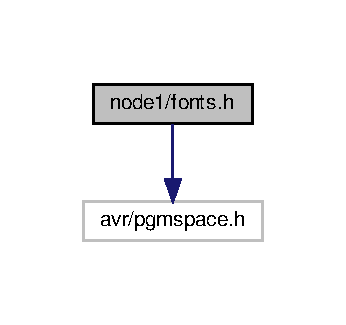
\includegraphics[width=166pt]{fonts_8h__incl}
\end{center}
\end{figure}
This graph shows which files directly or indirectly include this file\+:\nopagebreak
\begin{figure}[H]
\begin{center}
\leavevmode
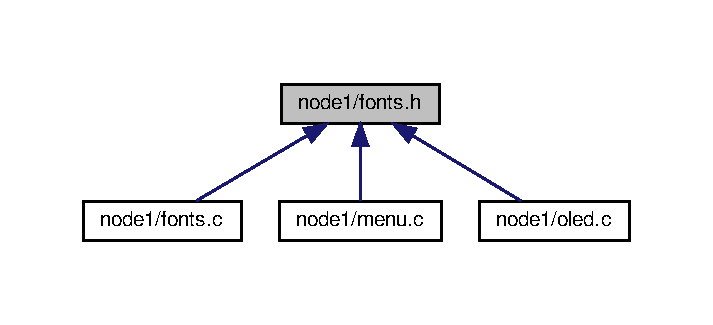
\includegraphics[width=342pt]{fonts_8h__dep__incl}
\end{center}
\end{figure}
\subsection*{Variables}
\begin{DoxyCompactItemize}
\item 
\mbox{\Hypertarget{fonts_8h_ae43c5fc2e1d3b49eb7f3f1c7166bd81d}\label{fonts_8h_ae43c5fc2e1d3b49eb7f3f1c7166bd81d}} 
const unsigned char P\+R\+O\+G\+M\+EM \hyperlink{fonts_8h_ae43c5fc2e1d3b49eb7f3f1c7166bd81d}{font8} \mbox{[}95\mbox{]}\mbox{[}8\mbox{]}
\begin{DoxyCompactList}\small\item\em Large font, 8x8. \end{DoxyCompactList}\end{DoxyCompactItemize}


\subsection{Detailed Description}
Module with font for printing to the O\+L\+ED screen. 


\hypertarget{node1_2fsm_8h}{}\section{node1/fsm.h File Reference}
\label{node1_2fsm_8h}\index{node1/fsm.\+h@{node1/fsm.\+h}}


Module for running the system as a Finite State Machine.  


{\ttfamily \#include \char`\"{}../common/fsm\+\_\+state.\+h\char`\"{}}\newline
Include dependency graph for fsm.\+h\+:
\nopagebreak
\begin{figure}[H]
\begin{center}
\leavevmode
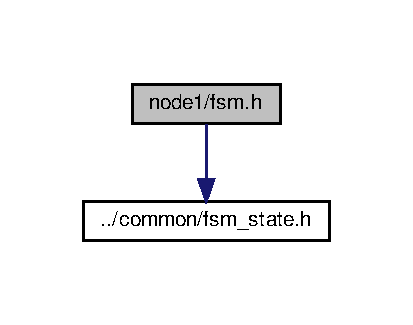
\includegraphics[width=198pt]{node1_2fsm_8h__incl}
\end{center}
\end{figure}
This graph shows which files directly or indirectly include this file\+:\nopagebreak
\begin{figure}[H]
\begin{center}
\leavevmode
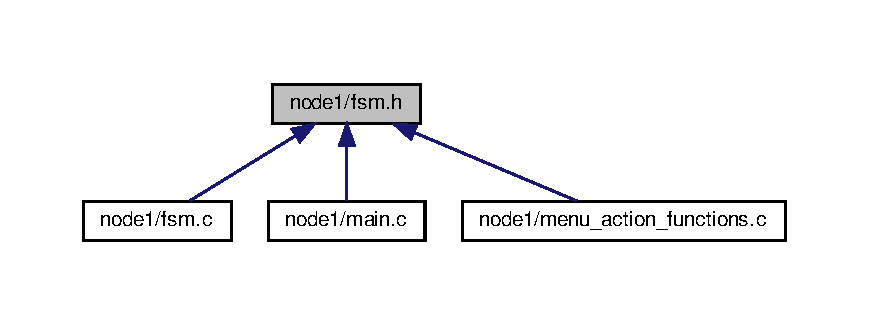
\includegraphics[width=350pt]{node1_2fsm_8h__dep__incl}
\end{center}
\end{figure}
\subsection*{Functions}
\begin{DoxyCompactItemize}
\item 
F\+S\+M\+\_\+\+S\+T\+A\+TE \hyperlink{node1_2fsm_8h_a738db290745f8f50938f482a5da85f37}{fsm\+\_\+get\+\_\+state} (void)
\begin{DoxyCompactList}\small\item\em Returns the current F\+SM state. \end{DoxyCompactList}\item 
void \hyperlink{node1_2fsm_8h_a10da0d27428fd76c537c3bdb468c7816}{fsm\+\_\+transition\+\_\+to} (F\+S\+M\+\_\+\+S\+T\+A\+TE state)
\begin{DoxyCompactList}\small\item\em Transitions the F\+SM to {\ttfamily state} by calling the state\textquotesingle{}s entry actions, and updating the current state. \end{DoxyCompactList}\item 
unsigned int \hyperlink{node1_2fsm_8h_a9926003a1b6faa1f0ce31b5976b5bf16}{fsm\+\_\+get\+\_\+lives\+\_\+left} (void)
\begin{DoxyCompactList}\small\item\em Returns the number of lives left in a game. \end{DoxyCompactList}\item 
void \hyperlink{node1_2fsm_8h_a29847c00ae4183b4838b94dc4111b11b}{fsm\+\_\+set\+\_\+lives\+\_\+left} (unsigned int lives)
\begin{DoxyCompactList}\small\item\em Sets the number of lives left in a game. \end{DoxyCompactList}\end{DoxyCompactItemize}


\subsection{Detailed Description}
Module for running the system as a Finite State Machine. 



\subsection{Function Documentation}
\mbox{\Hypertarget{node1_2fsm_8h_a9926003a1b6faa1f0ce31b5976b5bf16}\label{node1_2fsm_8h_a9926003a1b6faa1f0ce31b5976b5bf16}} 
\index{node1/fsm.\+h@{node1/fsm.\+h}!fsm\+\_\+get\+\_\+lives\+\_\+left@{fsm\+\_\+get\+\_\+lives\+\_\+left}}
\index{fsm\+\_\+get\+\_\+lives\+\_\+left@{fsm\+\_\+get\+\_\+lives\+\_\+left}!node1/fsm.\+h@{node1/fsm.\+h}}
\subsubsection{\texorpdfstring{fsm\+\_\+get\+\_\+lives\+\_\+left()}{fsm\_get\_lives\_left()}}
{\footnotesize\ttfamily unsigned int fsm\+\_\+get\+\_\+lives\+\_\+left (\begin{DoxyParamCaption}\item[{void}]{ }\end{DoxyParamCaption})}



Returns the number of lives left in a game. 

\begin{DoxyReturn}{Returns}
The number of lives left in a game. 
\end{DoxyReturn}


Definition at line 31 of file fsm.\+c.

\mbox{\Hypertarget{node1_2fsm_8h_a738db290745f8f50938f482a5da85f37}\label{node1_2fsm_8h_a738db290745f8f50938f482a5da85f37}} 
\index{node1/fsm.\+h@{node1/fsm.\+h}!fsm\+\_\+get\+\_\+state@{fsm\+\_\+get\+\_\+state}}
\index{fsm\+\_\+get\+\_\+state@{fsm\+\_\+get\+\_\+state}!node1/fsm.\+h@{node1/fsm.\+h}}
\subsubsection{\texorpdfstring{fsm\+\_\+get\+\_\+state()}{fsm\_get\_state()}}
{\footnotesize\ttfamily F\+S\+M\+\_\+\+S\+T\+A\+TE fsm\+\_\+get\+\_\+state (\begin{DoxyParamCaption}\item[{void}]{ }\end{DoxyParamCaption})}



Returns the current F\+SM state. 

\begin{DoxyReturn}{Returns}
The current F\+SM state, of data type {\ttfamily F\+S\+M\+\_\+\+S\+T\+A\+TE}. 
\end{DoxyReturn}


Definition at line 26 of file fsm.\+c.

\mbox{\Hypertarget{node1_2fsm_8h_a29847c00ae4183b4838b94dc4111b11b}\label{node1_2fsm_8h_a29847c00ae4183b4838b94dc4111b11b}} 
\index{node1/fsm.\+h@{node1/fsm.\+h}!fsm\+\_\+set\+\_\+lives\+\_\+left@{fsm\+\_\+set\+\_\+lives\+\_\+left}}
\index{fsm\+\_\+set\+\_\+lives\+\_\+left@{fsm\+\_\+set\+\_\+lives\+\_\+left}!node1/fsm.\+h@{node1/fsm.\+h}}
\subsubsection{\texorpdfstring{fsm\+\_\+set\+\_\+lives\+\_\+left()}{fsm\_set\_lives\_left()}}
{\footnotesize\ttfamily void fsm\+\_\+set\+\_\+lives\+\_\+left (\begin{DoxyParamCaption}\item[{unsigned int}]{lives }\end{DoxyParamCaption})}



Sets the number of lives left in a game. 


\begin{DoxyParams}{Parameters}
{\em lives\+\_\+left} & The new number of lives left in a game. \\
\hline
\end{DoxyParams}


Definition at line 36 of file fsm.\+c.

\mbox{\Hypertarget{node1_2fsm_8h_a10da0d27428fd76c537c3bdb468c7816}\label{node1_2fsm_8h_a10da0d27428fd76c537c3bdb468c7816}} 
\index{node1/fsm.\+h@{node1/fsm.\+h}!fsm\+\_\+transition\+\_\+to@{fsm\+\_\+transition\+\_\+to}}
\index{fsm\+\_\+transition\+\_\+to@{fsm\+\_\+transition\+\_\+to}!node1/fsm.\+h@{node1/fsm.\+h}}
\subsubsection{\texorpdfstring{fsm\+\_\+transition\+\_\+to()}{fsm\_transition\_to()}}
{\footnotesize\ttfamily void fsm\+\_\+transition\+\_\+to (\begin{DoxyParamCaption}\item[{F\+S\+M\+\_\+\+S\+T\+A\+TE}]{state }\end{DoxyParamCaption})}



Transitions the F\+SM to {\ttfamily state} by calling the state\textquotesingle{}s entry actions, and updating the current state. 


\begin{DoxyParams}{Parameters}
{\em state} & The F\+SM state to be transitioned to, of data type {\ttfamily F\+S\+M\+\_\+\+S\+T\+A\+TE}. \\
\hline
\end{DoxyParams}


Definition at line 41 of file fsm.\+c.


\hypertarget{node2_2fsm_8h}{}\section{node2/fsm.h File Reference}
\label{node2_2fsm_8h}\index{node2/fsm.\+h@{node2/fsm.\+h}}


Module consisting of state-\/machine-\/functionality.  


{\ttfamily \#include \char`\"{}../common/fsm\+\_\+state.\+h\char`\"{}}\newline
Include dependency graph for fsm.\+h\+:
\nopagebreak
\begin{figure}[H]
\begin{center}
\leavevmode
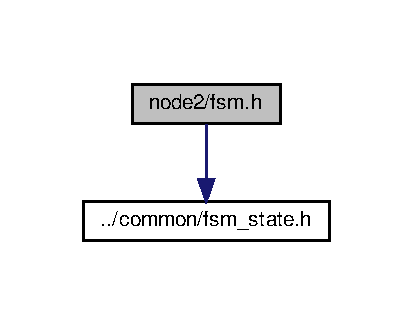
\includegraphics[width=198pt]{node2_2fsm_8h__incl}
\end{center}
\end{figure}
This graph shows which files directly or indirectly include this file\+:\nopagebreak
\begin{figure}[H]
\begin{center}
\leavevmode
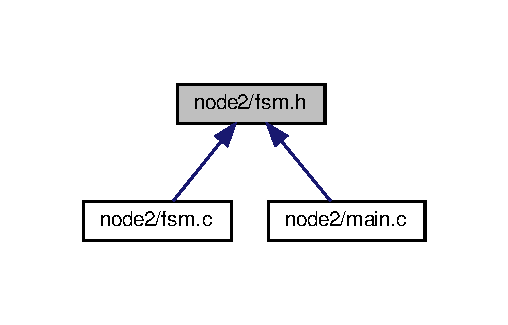
\includegraphics[width=244pt]{node2_2fsm_8h__dep__incl}
\end{center}
\end{figure}
\subsection*{Functions}
\begin{DoxyCompactItemize}
\item 
F\+S\+M\+\_\+\+S\+T\+A\+TE \hyperlink{node2_2fsm_8h_aa4e82e4c25771d31ae375834c3a2df75}{fsm\+\_\+get\+\_\+state} ()
\begin{DoxyCompactList}\small\item\em Returns the current F\+SM state. \end{DoxyCompactList}\item 
void \hyperlink{node2_2fsm_8h_a10da0d27428fd76c537c3bdb468c7816}{fsm\+\_\+transition\+\_\+to} (F\+S\+M\+\_\+\+S\+T\+A\+TE state)
\begin{DoxyCompactList}\small\item\em Transitions the F\+SM to {\ttfamily state} by calling the state\textquotesingle{}s entry actions, and updating the current state. \end{DoxyCompactList}\end{DoxyCompactItemize}


\subsection{Detailed Description}
Module consisting of state-\/machine-\/functionality. 



\subsection{Function Documentation}
\mbox{\Hypertarget{node2_2fsm_8h_aa4e82e4c25771d31ae375834c3a2df75}\label{node2_2fsm_8h_aa4e82e4c25771d31ae375834c3a2df75}} 
\index{node2/fsm.\+h@{node2/fsm.\+h}!fsm\+\_\+get\+\_\+state@{fsm\+\_\+get\+\_\+state}}
\index{fsm\+\_\+get\+\_\+state@{fsm\+\_\+get\+\_\+state}!node2/fsm.\+h@{node2/fsm.\+h}}
\subsubsection{\texorpdfstring{fsm\+\_\+get\+\_\+state()}{fsm\_get\_state()}}
{\footnotesize\ttfamily F\+S\+M\+\_\+\+S\+T\+A\+TE fsm\+\_\+get\+\_\+state (\begin{DoxyParamCaption}{ }\end{DoxyParamCaption})}



Returns the current F\+SM state. 

\begin{DoxyReturn}{Returns}
The current F\+SM state, of data type {\ttfamily F\+S\+M\+\_\+\+S\+T\+A\+TE}. 
\end{DoxyReturn}


Definition at line 26 of file fsm.\+c.

\mbox{\Hypertarget{node2_2fsm_8h_a10da0d27428fd76c537c3bdb468c7816}\label{node2_2fsm_8h_a10da0d27428fd76c537c3bdb468c7816}} 
\index{node2/fsm.\+h@{node2/fsm.\+h}!fsm\+\_\+transition\+\_\+to@{fsm\+\_\+transition\+\_\+to}}
\index{fsm\+\_\+transition\+\_\+to@{fsm\+\_\+transition\+\_\+to}!node2/fsm.\+h@{node2/fsm.\+h}}
\subsubsection{\texorpdfstring{fsm\+\_\+transition\+\_\+to()}{fsm\_transition\_to()}}
{\footnotesize\ttfamily void fsm\+\_\+transition\+\_\+to (\begin{DoxyParamCaption}\item[{F\+S\+M\+\_\+\+S\+T\+A\+TE}]{state }\end{DoxyParamCaption})}



Transitions the F\+SM to {\ttfamily state} by calling the state\textquotesingle{}s entry actions, and updating the current state. 


\begin{DoxyParams}{Parameters}
{\em state} & The F\+SM state to be transitioned to, of data type {\ttfamily F\+S\+M\+\_\+\+S\+T\+A\+TE}. \\
\hline
\end{DoxyParams}


Definition at line 41 of file fsm.\+c.


\hypertarget{highscore_8h}{}\section{node1/highscore.h File Reference}
\label{highscore_8h}\index{node1/highscore.\+h@{node1/highscore.\+h}}


Module for saving and updating highscores in the non-\/volatile E\+E\+P\+R\+OM.  


{\ttfamily \#include $<$stdint.\+h$>$}\newline
Include dependency graph for highscore.\+h\+:\nopagebreak
\begin{figure}[H]
\begin{center}
\leavevmode
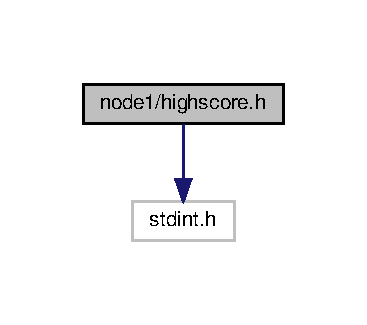
\includegraphics[width=176pt]{highscore_8h__incl}
\end{center}
\end{figure}
This graph shows which files directly or indirectly include this file\+:\nopagebreak
\begin{figure}[H]
\begin{center}
\leavevmode
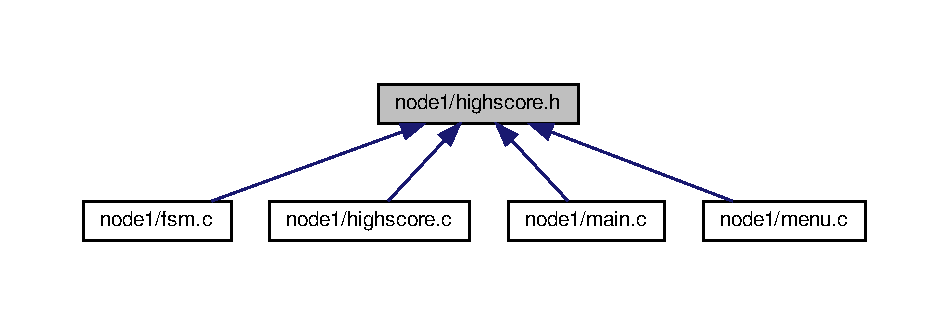
\includegraphics[width=350pt]{highscore_8h__dep__incl}
\end{center}
\end{figure}
\subsection*{Macros}
\begin{DoxyCompactItemize}
\item 
\mbox{\Hypertarget{highscore_8h_a15d1ac1fca3799b4aa6ee5b94dd7dd97}\label{highscore_8h_a15d1ac1fca3799b4aa6ee5b94dd7dd97}} 
\#define {\bfseries H\+I\+G\+H\+S\+C\+O\+R\+E\+\_\+\+L\+I\+S\+T\+\_\+\+L\+E\+N\+G\+TH}~3
\end{DoxyCompactItemize}
\subsection*{Functions}
\begin{DoxyCompactItemize}
\item 
\mbox{\Hypertarget{highscore_8h_afb784b5df2d71aa32f62c632a4f1951a}\label{highscore_8h_afb784b5df2d71aa32f62c632a4f1951a}} 
void \hyperlink{highscore_8h_afb784b5df2d71aa32f62c632a4f1951a}{highscore\+\_\+init} (void)
\begin{DoxyCompactList}\small\item\em Initiates the highscore by reading the highscore table from the E\+E\+P\+R\+OM memory. \end{DoxyCompactList}\item 
\mbox{\Hypertarget{highscore_8h_a5475f5fa2206bd5bcdbb5b96a6f0ca49}\label{highscore_8h_a5475f5fa2206bd5bcdbb5b96a6f0ca49}} 
void \hyperlink{highscore_8h_a5475f5fa2206bd5bcdbb5b96a6f0ca49}{highscore\+\_\+update} (void)
\begin{DoxyCompactList}\small\item\em Updates the highscore, by comparing any new set scores to the highscore table. \end{DoxyCompactList}\item 
uint16\+\_\+t $\ast$ \hyperlink{highscore_8h_a13b610af1ff392fc51e1f6f4e8cc7425}{highscore\+\_\+get} (void)
\begin{DoxyCompactList}\small\item\em Returns the highscore table. \end{DoxyCompactList}\item 
\mbox{\Hypertarget{highscore_8h_afa0fa6095ee9f0bbdeb155d11e233d1a}\label{highscore_8h_afa0fa6095ee9f0bbdeb155d11e233d1a}} 
void \hyperlink{highscore_8h_afa0fa6095ee9f0bbdeb155d11e233d1a}{highscore\+\_\+reset} (void)
\begin{DoxyCompactList}\small\item\em Resets the highscore table, setting all highscores to 0. \end{DoxyCompactList}\item 
\mbox{\Hypertarget{highscore_8h_ad1447bafdf8c9142d3ae2c2b08a97945}\label{highscore_8h_ad1447bafdf8c9142d3ae2c2b08a97945}} 
void \hyperlink{highscore_8h_ad1447bafdf8c9142d3ae2c2b08a97945}{highscore\+\_\+set\+\_\+new\+\_\+score} (uint16\+\_\+t score)
\begin{DoxyCompactList}\small\item\em Sets a new score, which is compared to the highscore table when {\ttfamily \hyperlink{highscore_8h_a5475f5fa2206bd5bcdbb5b96a6f0ca49}{highscore\+\_\+update()}} is called. \end{DoxyCompactList}\end{DoxyCompactItemize}


\subsection{Detailed Description}
Module for saving and updating highscores in the non-\/volatile E\+E\+P\+R\+OM. 



\subsection{Function Documentation}
\mbox{\Hypertarget{highscore_8h_a13b610af1ff392fc51e1f6f4e8cc7425}\label{highscore_8h_a13b610af1ff392fc51e1f6f4e8cc7425}} 
\index{highscore.\+h@{highscore.\+h}!highscore\+\_\+get@{highscore\+\_\+get}}
\index{highscore\+\_\+get@{highscore\+\_\+get}!highscore.\+h@{highscore.\+h}}
\subsubsection{\texorpdfstring{highscore\+\_\+get()}{highscore\_get()}}
{\footnotesize\ttfamily uint16\+\_\+t$\ast$ highscore\+\_\+get (\begin{DoxyParamCaption}\item[{void}]{ }\end{DoxyParamCaption})}



Returns the highscore table. 

\begin{DoxyReturn}{Returns}
The highscore table, as an array with three elements of type {\ttfamily uint16\+\_\+t}. 
\end{DoxyReturn}


Definition at line 55 of file highscore.\+c.


\hypertarget{node1_2main_8c}{}\section{node1/main.c File Reference}
\label{node1_2main_8c}\index{node1/main.\+c@{node1/main.\+c}}


Main program of node 1.  


{\ttfamily \#include \char`\"{}uart.\+h\char`\"{}}\newline
{\ttfamily \#include \char`\"{}sram.\+h\char`\"{}}\newline
{\ttfamily \#include \char`\"{}user\+\_\+input.\+h\char`\"{}}\newline
{\ttfamily \#include \char`\"{}oled.\+h\char`\"{}}\newline
{\ttfamily \#include \char`\"{}menu.\+h\char`\"{}}\newline
{\ttfamily \#include \char`\"{}can\+\_\+driver.\+h\char`\"{}}\newline
{\ttfamily \#include \char`\"{}highscore.\+h\char`\"{}}\newline
{\ttfamily \#include \char`\"{}fsm.\+h\char`\"{}}\newline
{\ttfamily \#include \char`\"{}../common/can.\+h\char`\"{}}\newline
{\ttfamily \#include $<$avr/interrupt.\+h$>$}\newline
{\ttfamily \#include $<$util/delay.\+h$>$}\newline
Include dependency graph for main.\+c\+:
\nopagebreak
\begin{figure}[H]
\begin{center}
\leavevmode
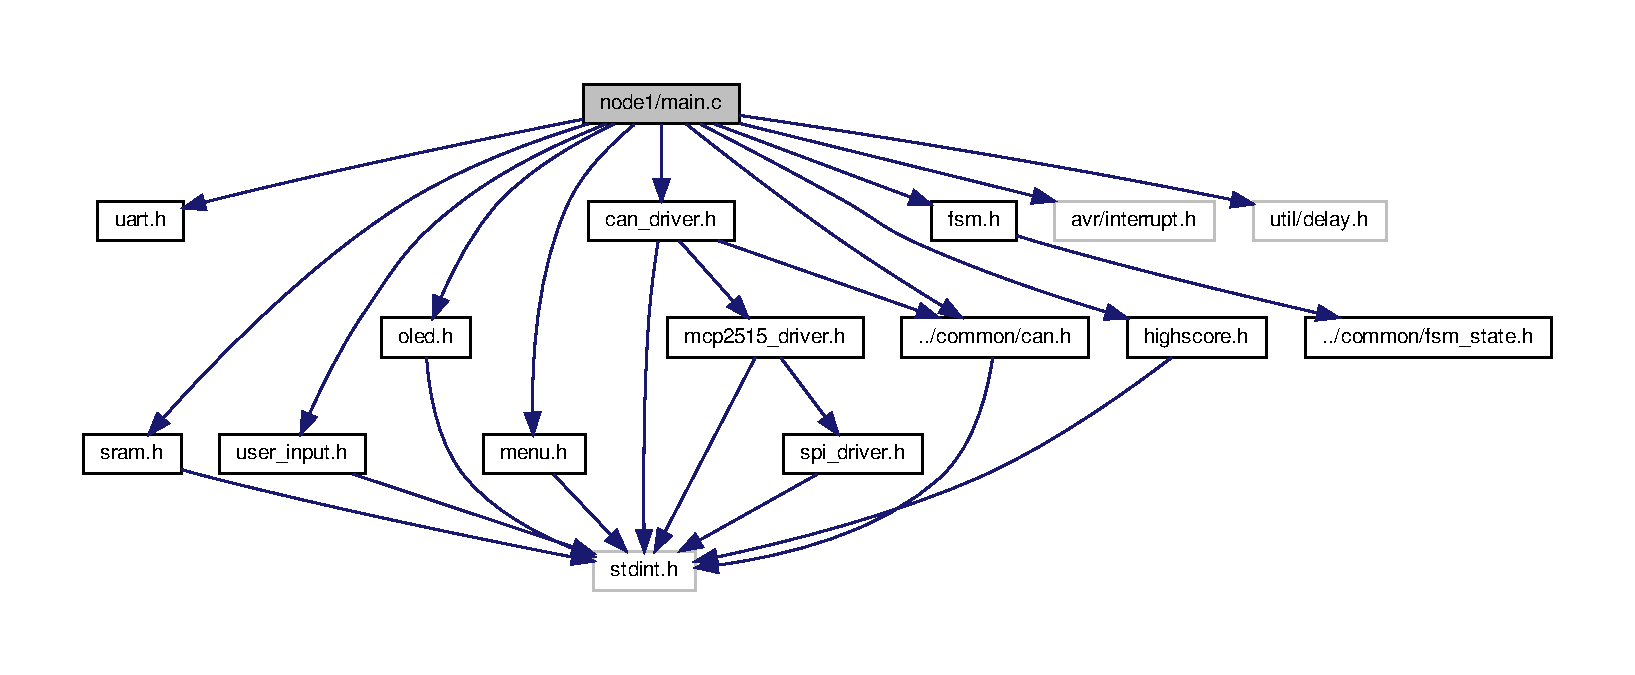
\includegraphics[width=350pt]{node1_2main_8c__incl}
\end{center}
\end{figure}
\subsection*{Macros}
\begin{DoxyCompactItemize}
\item 
\mbox{\Hypertarget{node1_2main_8c_a43bafb28b29491ec7f871319b5a3b2f8}\label{node1_2main_8c_a43bafb28b29491ec7f871319b5a3b2f8}} 
\#define {\bfseries F\+\_\+\+C\+PU}~4.\+9152\+E6
\item 
\mbox{\Hypertarget{node1_2main_8c_a62634036639f88eece6fbf226b45f84b}\label{node1_2main_8c_a62634036639f88eece6fbf226b45f84b}} 
\#define {\bfseries B\+A\+UD}~9600
\item 
\mbox{\Hypertarget{node1_2main_8c_af85b10a3b65a3b2c909578fd6601e95e}\label{node1_2main_8c_af85b10a3b65a3b2c909578fd6601e95e}} 
\#define {\bfseries U\+B\+RR}~F\+\_\+\+C\+PU / 16 / B\+A\+UD -\/ 1
\item 
\mbox{\Hypertarget{node1_2main_8c_ab5df03a8a29c9c55a0fbdea399da5626}\label{node1_2main_8c_ab5df03a8a29c9c55a0fbdea399da5626}} 
\#define {\bfseries N\+U\+M\+B\+E\+R\+\_\+\+O\+F\+\_\+\+L\+I\+V\+ES}~3
\end{DoxyCompactItemize}
\subsection*{Functions}
\begin{DoxyCompactItemize}
\item 
\mbox{\Hypertarget{node1_2main_8c_ae66f6b31b5ad750f1fe042a706a4e3d4}\label{node1_2main_8c_ae66f6b31b5ad750f1fe042a706a4e3d4}} 
int {\bfseries main} ()
\item 
\mbox{\Hypertarget{node1_2main_8c_afea150fcd685610cb9f7672fce361e53}\label{node1_2main_8c_afea150fcd685610cb9f7672fce361e53}} 
{\bfseries I\+SR} (I\+N\+T0\+\_\+vect)
\item 
\mbox{\Hypertarget{node1_2main_8c_ad39420cdd896dd12c68e36313139d0a5}\label{node1_2main_8c_ad39420cdd896dd12c68e36313139d0a5}} 
{\bfseries I\+SR} (T\+I\+M\+E\+R1\+\_\+\+C\+O\+M\+P\+A\+\_\+vect)
\item 
\mbox{\Hypertarget{node1_2main_8c_a86953738188622410b88938da2bf8a63}\label{node1_2main_8c_a86953738188622410b88938da2bf8a63}} 
{\bfseries I\+SR} (T\+I\+M\+E\+R3\+\_\+\+C\+O\+M\+P\+A\+\_\+vect)
\item 
\mbox{\Hypertarget{node1_2main_8c_a04d3f94da90f7ac1b018f80f321e86de}\label{node1_2main_8c_a04d3f94da90f7ac1b018f80f321e86de}} 
{\bfseries I\+SR} (B\+A\+D\+I\+S\+R\+\_\+vect)
\end{DoxyCompactItemize}


\subsection{Detailed Description}
Main program of node 1. 


\hypertarget{node2_2main_8c}{}\section{node2/main.c File Reference}
\label{node2_2main_8c}\index{node2/main.\+c@{node2/main.\+c}}


Main program of node 2.  


{\ttfamily \#include \char`\"{}uart\+\_\+and\+\_\+printf/uart.\+h\char`\"{}}\newline
{\ttfamily \#include \char`\"{}uart\+\_\+and\+\_\+printf/printf-\/stdarg.\+h\char`\"{}}\newline
{\ttfamily \#include \char`\"{}can/can\+\_\+controller.\+h\char`\"{}}\newline
{\ttfamily \#include \char`\"{}sam/sam3x/include/sam.\+h\char`\"{}}\newline
{\ttfamily \#include \char`\"{}game.\+h\char`\"{}}\newline
{\ttfamily \#include \char`\"{}fsm.\+h\char`\"{}}\newline
Include dependency graph for main.\+c\+:
\nopagebreak
\begin{figure}[H]
\begin{center}
\leavevmode
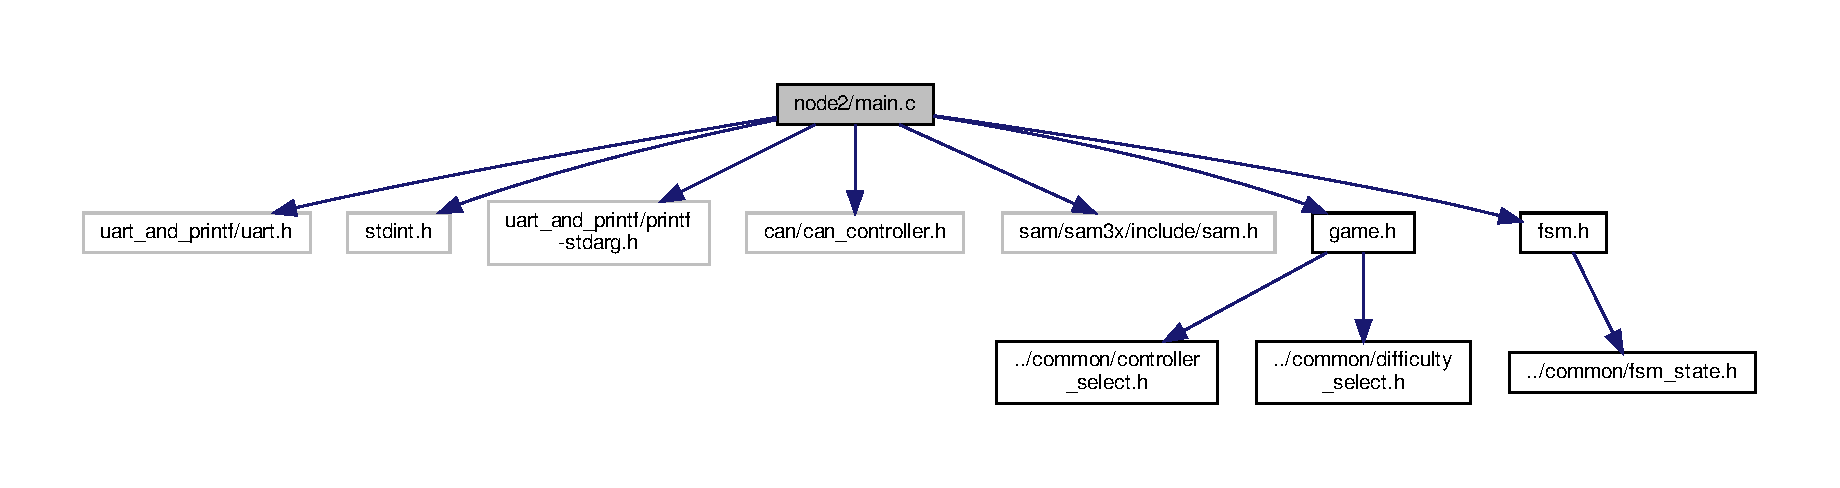
\includegraphics[width=350pt]{node2_2main_8c__incl}
\end{center}
\end{figure}
\subsection*{Functions}
\begin{DoxyCompactItemize}
\item 
\mbox{\Hypertarget{node2_2main_8c_ae66f6b31b5ad750f1fe042a706a4e3d4}\label{node2_2main_8c_ae66f6b31b5ad750f1fe042a706a4e3d4}} 
int {\bfseries main} ()
\end{DoxyCompactItemize}


\subsection{Detailed Description}
Main program of node 2. 


\hypertarget{mcp2515__driver_8h}{}\section{node1/mcp2515\+\_\+driver.h File Reference}
\label{mcp2515__driver_8h}\index{node1/mcp2515\+\_\+driver.\+h@{node1/mcp2515\+\_\+driver.\+h}}


Module for controlling the sending and receiving data over the C\+AN bus.  


{\ttfamily \#include \char`\"{}spi\+\_\+driver.\+h\char`\"{}}\newline
{\ttfamily \#include $<$stdint.\+h$>$}\newline
Include dependency graph for mcp2515\+\_\+driver.\+h\+:\nopagebreak
\begin{figure}[H]
\begin{center}
\leavevmode
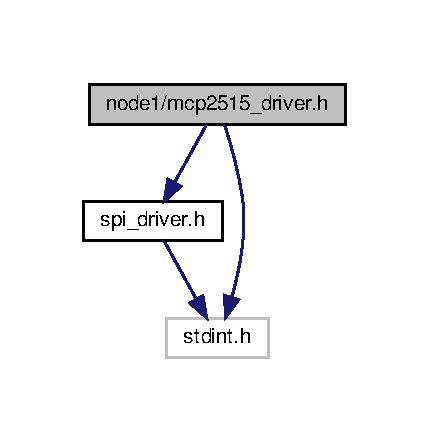
\includegraphics[width=206pt]{mcp2515__driver_8h__incl}
\end{center}
\end{figure}
This graph shows which files directly or indirectly include this file\+:\nopagebreak
\begin{figure}[H]
\begin{center}
\leavevmode
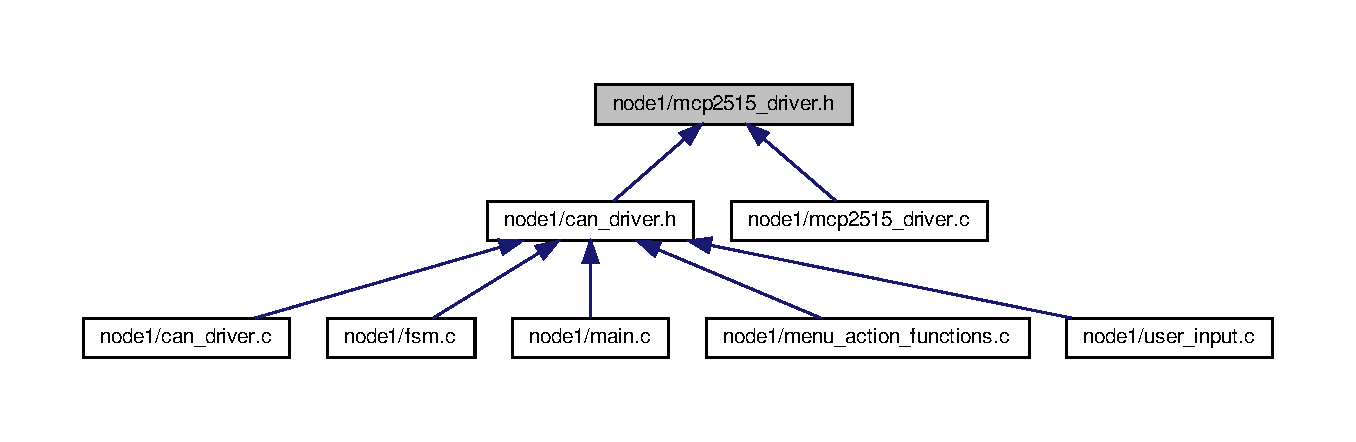
\includegraphics[width=350pt]{mcp2515__driver_8h__dep__incl}
\end{center}
\end{figure}
\subsection*{Macros}
\begin{DoxyCompactItemize}
\item 
\mbox{\Hypertarget{mcp2515__driver_8h_ae421a063d5c9a67484389eb3eaebebfd}\label{mcp2515__driver_8h_ae421a063d5c9a67484389eb3eaebebfd}} 
\#define {\bfseries M\+C\+P\+\_\+\+R\+X\+F0\+S\+I\+DH}~0x00
\item 
\mbox{\Hypertarget{mcp2515__driver_8h_a9c93381116e954e7a310e2dbbd2dbc4e}\label{mcp2515__driver_8h_a9c93381116e954e7a310e2dbbd2dbc4e}} 
\#define {\bfseries M\+C\+P\+\_\+\+R\+X\+F0\+S\+I\+DL}~0x01
\item 
\mbox{\Hypertarget{mcp2515__driver_8h_a1ec986ef1512da764c3394f50522b16b}\label{mcp2515__driver_8h_a1ec986ef1512da764c3394f50522b16b}} 
\#define {\bfseries M\+C\+P\+\_\+\+R\+X\+F0\+E\+I\+D8}~0x02
\item 
\mbox{\Hypertarget{mcp2515__driver_8h_a3de3114c44a811cbaabf1861ba55a690}\label{mcp2515__driver_8h_a3de3114c44a811cbaabf1861ba55a690}} 
\#define {\bfseries M\+C\+P\+\_\+\+R\+X\+F0\+E\+I\+D0}~0x03
\item 
\mbox{\Hypertarget{mcp2515__driver_8h_a0e86a1817cd0b31a287b150dd322f972}\label{mcp2515__driver_8h_a0e86a1817cd0b31a287b150dd322f972}} 
\#define {\bfseries M\+C\+P\+\_\+\+R\+X\+F1\+S\+I\+DH}~0x04
\item 
\mbox{\Hypertarget{mcp2515__driver_8h_ab57c15509135349cfac67fd74071cf01}\label{mcp2515__driver_8h_ab57c15509135349cfac67fd74071cf01}} 
\#define {\bfseries M\+C\+P\+\_\+\+R\+X\+F1\+S\+I\+DL}~0x05
\item 
\mbox{\Hypertarget{mcp2515__driver_8h_aecfcc2d9cddf17106316db150ac56f82}\label{mcp2515__driver_8h_aecfcc2d9cddf17106316db150ac56f82}} 
\#define {\bfseries M\+C\+P\+\_\+\+R\+X\+F1\+E\+I\+D8}~0x06
\item 
\mbox{\Hypertarget{mcp2515__driver_8h_a00edc9ebc006d15149797e48b82949c6}\label{mcp2515__driver_8h_a00edc9ebc006d15149797e48b82949c6}} 
\#define {\bfseries M\+C\+P\+\_\+\+R\+X\+F1\+E\+I\+D0}~0x07
\item 
\mbox{\Hypertarget{mcp2515__driver_8h_a2961fd5700a7ae397d71911f328799e3}\label{mcp2515__driver_8h_a2961fd5700a7ae397d71911f328799e3}} 
\#define {\bfseries M\+C\+P\+\_\+\+R\+X\+F2\+S\+I\+DH}~0x08
\item 
\mbox{\Hypertarget{mcp2515__driver_8h_a7fc1958385a3995ca062fba4ff14cb41}\label{mcp2515__driver_8h_a7fc1958385a3995ca062fba4ff14cb41}} 
\#define {\bfseries M\+C\+P\+\_\+\+R\+X\+F2\+S\+I\+DL}~0x09
\item 
\mbox{\Hypertarget{mcp2515__driver_8h_a31643cf05e789b655d0bf66c100fc5ae}\label{mcp2515__driver_8h_a31643cf05e789b655d0bf66c100fc5ae}} 
\#define {\bfseries M\+C\+P\+\_\+\+R\+X\+F2\+E\+I\+D8}~0x0A
\item 
\mbox{\Hypertarget{mcp2515__driver_8h_ad9666d49e084c975e49d1f9f7c3df20a}\label{mcp2515__driver_8h_ad9666d49e084c975e49d1f9f7c3df20a}} 
\#define {\bfseries M\+C\+P\+\_\+\+R\+X\+F2\+E\+I\+D0}~0x0B
\item 
\mbox{\Hypertarget{mcp2515__driver_8h_a1a470d80ae3644bf02f2cd4a7bb6aa39}\label{mcp2515__driver_8h_a1a470d80ae3644bf02f2cd4a7bb6aa39}} 
\#define {\bfseries M\+C\+P\+\_\+\+C\+A\+N\+S\+T\+AT}~0x0E
\item 
\mbox{\Hypertarget{mcp2515__driver_8h_a25864642b445cbfbd85f2a1a22947558}\label{mcp2515__driver_8h_a25864642b445cbfbd85f2a1a22947558}} 
\#define {\bfseries M\+C\+P\+\_\+\+C\+A\+N\+C\+T\+RL}~0x0F
\item 
\mbox{\Hypertarget{mcp2515__driver_8h_a21d7a29b957697c7d35f7a6a8ab6fba7}\label{mcp2515__driver_8h_a21d7a29b957697c7d35f7a6a8ab6fba7}} 
\#define {\bfseries M\+C\+P\+\_\+\+R\+X\+F3\+S\+I\+DH}~0x10
\item 
\mbox{\Hypertarget{mcp2515__driver_8h_a71d3d35f05bf08e68523a9efc61cfbfc}\label{mcp2515__driver_8h_a71d3d35f05bf08e68523a9efc61cfbfc}} 
\#define {\bfseries M\+C\+P\+\_\+\+R\+X\+F3\+S\+I\+DL}~0x11
\item 
\mbox{\Hypertarget{mcp2515__driver_8h_aec6f10e1f16aa75cf9a2c45cbf072c0c}\label{mcp2515__driver_8h_aec6f10e1f16aa75cf9a2c45cbf072c0c}} 
\#define {\bfseries M\+C\+P\+\_\+\+R\+X\+F3\+E\+I\+D8}~0x12
\item 
\mbox{\Hypertarget{mcp2515__driver_8h_ae6d1393bf6ade012e9de52ce3f781cc0}\label{mcp2515__driver_8h_ae6d1393bf6ade012e9de52ce3f781cc0}} 
\#define {\bfseries M\+C\+P\+\_\+\+R\+X\+F3\+E\+I\+D0}~0x13
\item 
\mbox{\Hypertarget{mcp2515__driver_8h_a870788013a5eb433261fb4bbe755b798}\label{mcp2515__driver_8h_a870788013a5eb433261fb4bbe755b798}} 
\#define {\bfseries M\+C\+P\+\_\+\+R\+X\+F4\+S\+I\+DH}~0x14
\item 
\mbox{\Hypertarget{mcp2515__driver_8h_a26ea2d067a97a328bdb355f5a1f9bcae}\label{mcp2515__driver_8h_a26ea2d067a97a328bdb355f5a1f9bcae}} 
\#define {\bfseries M\+C\+P\+\_\+\+R\+X\+F4\+S\+I\+DL}~0x15
\item 
\mbox{\Hypertarget{mcp2515__driver_8h_a3b8889cb0efb5374525dc60f8faa6e35}\label{mcp2515__driver_8h_a3b8889cb0efb5374525dc60f8faa6e35}} 
\#define {\bfseries M\+C\+P\+\_\+\+R\+X\+F4\+E\+I\+D8}~0x16
\item 
\mbox{\Hypertarget{mcp2515__driver_8h_a61e6e6a2b3c20e8d900bcb628854a404}\label{mcp2515__driver_8h_a61e6e6a2b3c20e8d900bcb628854a404}} 
\#define {\bfseries M\+C\+P\+\_\+\+R\+X\+F4\+E\+I\+D0}~0x17
\item 
\mbox{\Hypertarget{mcp2515__driver_8h_ac7bc37d5b6536d6c4c15d8a36483fe79}\label{mcp2515__driver_8h_ac7bc37d5b6536d6c4c15d8a36483fe79}} 
\#define {\bfseries M\+C\+P\+\_\+\+R\+X\+F5\+S\+I\+DH}~0x18
\item 
\mbox{\Hypertarget{mcp2515__driver_8h_ad4328ca7028ab38ac270f8547fb59582}\label{mcp2515__driver_8h_ad4328ca7028ab38ac270f8547fb59582}} 
\#define {\bfseries M\+C\+P\+\_\+\+R\+X\+F5\+S\+I\+DL}~0x19
\item 
\mbox{\Hypertarget{mcp2515__driver_8h_ac44d4ade53dbe90f58d28d54f3ea4aa0}\label{mcp2515__driver_8h_ac44d4ade53dbe90f58d28d54f3ea4aa0}} 
\#define {\bfseries M\+C\+P\+\_\+\+R\+X\+F5\+E\+I\+D8}~0x1A
\item 
\mbox{\Hypertarget{mcp2515__driver_8h_a0dee7fada196f7183e8f709df24e0bc4}\label{mcp2515__driver_8h_a0dee7fada196f7183e8f709df24e0bc4}} 
\#define {\bfseries M\+C\+P\+\_\+\+R\+X\+F5\+E\+I\+D0}~0x1B
\item 
\mbox{\Hypertarget{mcp2515__driver_8h_a408a3bfd90d57612646979a8b69497c4}\label{mcp2515__driver_8h_a408a3bfd90d57612646979a8b69497c4}} 
\#define {\bfseries M\+C\+P\+\_\+\+T\+EC}~0x1C
\item 
\mbox{\Hypertarget{mcp2515__driver_8h_a6f032cfd514ddf69f0bc8424cf924c4a}\label{mcp2515__driver_8h_a6f032cfd514ddf69f0bc8424cf924c4a}} 
\#define {\bfseries M\+C\+P\+\_\+\+R\+EC}~0x1D
\item 
\mbox{\Hypertarget{mcp2515__driver_8h_a74a0dc603b68c2ecbb63c3ed29010e17}\label{mcp2515__driver_8h_a74a0dc603b68c2ecbb63c3ed29010e17}} 
\#define {\bfseries M\+C\+P\+\_\+\+R\+X\+M0\+S\+I\+DH}~0x20
\item 
\mbox{\Hypertarget{mcp2515__driver_8h_acff5cba98baa23236a302a5b678d2899}\label{mcp2515__driver_8h_acff5cba98baa23236a302a5b678d2899}} 
\#define {\bfseries M\+C\+P\+\_\+\+R\+X\+M0\+S\+I\+DL}~0x21
\item 
\mbox{\Hypertarget{mcp2515__driver_8h_a0b72079ef3123f9384f8e8767c381086}\label{mcp2515__driver_8h_a0b72079ef3123f9384f8e8767c381086}} 
\#define {\bfseries M\+C\+P\+\_\+\+R\+X\+M0\+E\+I\+D8}~0x22
\item 
\mbox{\Hypertarget{mcp2515__driver_8h_a85951b834260f01b30915e446542d3ef}\label{mcp2515__driver_8h_a85951b834260f01b30915e446542d3ef}} 
\#define {\bfseries M\+C\+P\+\_\+\+R\+X\+M0\+E\+I\+D0}~0x23
\item 
\mbox{\Hypertarget{mcp2515__driver_8h_af33255d20e7adbb274843351676d15bd}\label{mcp2515__driver_8h_af33255d20e7adbb274843351676d15bd}} 
\#define {\bfseries M\+C\+P\+\_\+\+R\+X\+M1\+S\+I\+DH}~0x24
\item 
\mbox{\Hypertarget{mcp2515__driver_8h_abc4c9f616f34a1adef4dc2526ffeb95b}\label{mcp2515__driver_8h_abc4c9f616f34a1adef4dc2526ffeb95b}} 
\#define {\bfseries M\+C\+P\+\_\+\+R\+X\+M1\+S\+I\+DL}~0x25
\item 
\mbox{\Hypertarget{mcp2515__driver_8h_aac7b0eb43bfd43104e1876e9d75339b6}\label{mcp2515__driver_8h_aac7b0eb43bfd43104e1876e9d75339b6}} 
\#define {\bfseries M\+C\+P\+\_\+\+R\+X\+M1\+E\+I\+D8}~0x26
\item 
\mbox{\Hypertarget{mcp2515__driver_8h_ae384be8c5a58d1425449b1764ba3fdea}\label{mcp2515__driver_8h_ae384be8c5a58d1425449b1764ba3fdea}} 
\#define {\bfseries M\+C\+P\+\_\+\+R\+X\+M1\+E\+I\+D0}~0x27
\item 
\mbox{\Hypertarget{mcp2515__driver_8h_ad2e13220f9c51ccd5efda5d3c19761b8}\label{mcp2515__driver_8h_ad2e13220f9c51ccd5efda5d3c19761b8}} 
\#define {\bfseries M\+C\+P\+\_\+\+C\+N\+F3}~0x28
\item 
\mbox{\Hypertarget{mcp2515__driver_8h_a2a22ce749e287690e3d85514e2c7cb57}\label{mcp2515__driver_8h_a2a22ce749e287690e3d85514e2c7cb57}} 
\#define {\bfseries M\+C\+P\+\_\+\+C\+N\+F2}~0x29
\item 
\mbox{\Hypertarget{mcp2515__driver_8h_a0baef095a5a2997db4c75831e55e8e96}\label{mcp2515__driver_8h_a0baef095a5a2997db4c75831e55e8e96}} 
\#define {\bfseries M\+C\+P\+\_\+\+C\+N\+F1}~0x2A
\item 
\mbox{\Hypertarget{mcp2515__driver_8h_a778de33d21ab2eb875533a31a2e8ec69}\label{mcp2515__driver_8h_a778de33d21ab2eb875533a31a2e8ec69}} 
\#define {\bfseries M\+C\+P\+\_\+\+C\+A\+N\+I\+N\+TE}~0x2B
\item 
\mbox{\Hypertarget{mcp2515__driver_8h_ae82ca28239a27c2f8c4871e654480ee3}\label{mcp2515__driver_8h_ae82ca28239a27c2f8c4871e654480ee3}} 
\#define {\bfseries M\+C\+P\+\_\+\+C\+A\+N\+I\+N\+TF}~0x2C
\item 
\mbox{\Hypertarget{mcp2515__driver_8h_a1695d6e956775335641f7f600439919c}\label{mcp2515__driver_8h_a1695d6e956775335641f7f600439919c}} 
\#define {\bfseries M\+C\+P\+\_\+\+E\+F\+LG}~0x2D
\item 
\mbox{\Hypertarget{mcp2515__driver_8h_a8141153ac7a7a40b71f49a3e029c33ac}\label{mcp2515__driver_8h_a8141153ac7a7a40b71f49a3e029c33ac}} 
\#define {\bfseries M\+C\+P\+\_\+\+T\+X\+B0\+C\+T\+RL}~0x30
\item 
\mbox{\Hypertarget{mcp2515__driver_8h_a30d9219d01d77604bb8cccdb6bbb8a89}\label{mcp2515__driver_8h_a30d9219d01d77604bb8cccdb6bbb8a89}} 
\#define {\bfseries M\+C\+P\+\_\+\+T\+X\+B0\+S\+I\+DH}~0x31
\item 
\mbox{\Hypertarget{mcp2515__driver_8h_a64751f2c34434ba5c7cec9cb89bb3817}\label{mcp2515__driver_8h_a64751f2c34434ba5c7cec9cb89bb3817}} 
\#define {\bfseries M\+C\+P\+\_\+\+T\+X\+B0\+S\+I\+DL}~0x32
\item 
\mbox{\Hypertarget{mcp2515__driver_8h_a62c96077baaed616c41573046befe809}\label{mcp2515__driver_8h_a62c96077baaed616c41573046befe809}} 
\#define {\bfseries M\+C\+P\+\_\+\+T\+X\+B0\+E\+I\+D8}~0x33
\item 
\mbox{\Hypertarget{mcp2515__driver_8h_aa1f2c5ddd7fc55e3e184f5c31a0b0382}\label{mcp2515__driver_8h_aa1f2c5ddd7fc55e3e184f5c31a0b0382}} 
\#define {\bfseries M\+C\+P\+\_\+\+T\+X\+B0\+E\+I\+D0}~0x34
\item 
\mbox{\Hypertarget{mcp2515__driver_8h_af079eda36bde82cfee6ef43681813ec7}\label{mcp2515__driver_8h_af079eda36bde82cfee6ef43681813ec7}} 
\#define {\bfseries M\+C\+P\+\_\+\+T\+X\+B0\+D\+LC}~0x35
\item 
\mbox{\Hypertarget{mcp2515__driver_8h_aa37171b2eb1e0d9432c71b2b6a3ac879}\label{mcp2515__driver_8h_aa37171b2eb1e0d9432c71b2b6a3ac879}} 
\#define {\bfseries M\+C\+P\+\_\+\+T\+X\+B0\+D0}~0\+X36
\item 
\mbox{\Hypertarget{mcp2515__driver_8h_abc7ef66a386f13da6f893ea2f951693f}\label{mcp2515__driver_8h_abc7ef66a386f13da6f893ea2f951693f}} 
\#define {\bfseries M\+C\+P\+\_\+\+T\+X\+B1\+C\+T\+RL}~0x40
\item 
\mbox{\Hypertarget{mcp2515__driver_8h_a3aae8393ed1e6ea4da47cf3d1ab1f92e}\label{mcp2515__driver_8h_a3aae8393ed1e6ea4da47cf3d1ab1f92e}} 
\#define {\bfseries M\+C\+P\+\_\+\+T\+X\+B1\+S\+I\+DH}~0x41
\item 
\mbox{\Hypertarget{mcp2515__driver_8h_a1706fc81ff7ea86f107cca52588b52af}\label{mcp2515__driver_8h_a1706fc81ff7ea86f107cca52588b52af}} 
\#define {\bfseries M\+C\+P\+\_\+\+T\+X\+B1\+S\+I\+DL}~0x42
\item 
\mbox{\Hypertarget{mcp2515__driver_8h_ab63334c1f2a2ddd58564d2c8a9954272}\label{mcp2515__driver_8h_ab63334c1f2a2ddd58564d2c8a9954272}} 
\#define {\bfseries M\+C\+P\+\_\+\+T\+X\+B1\+E\+I\+D8}~0x43
\item 
\mbox{\Hypertarget{mcp2515__driver_8h_a1dfa1a69ad684ed9c15ff3ae3bc5d33f}\label{mcp2515__driver_8h_a1dfa1a69ad684ed9c15ff3ae3bc5d33f}} 
\#define {\bfseries M\+C\+P\+\_\+\+T\+X\+B1\+E\+I\+D0}~0x44
\item 
\mbox{\Hypertarget{mcp2515__driver_8h_ae1e6cf04674ca83b2ca0d01ba6465be0}\label{mcp2515__driver_8h_ae1e6cf04674ca83b2ca0d01ba6465be0}} 
\#define {\bfseries M\+C\+P\+\_\+\+T\+X\+B1\+D\+LC}~0x45
\item 
\mbox{\Hypertarget{mcp2515__driver_8h_a289812179d1f736b9b1e23c5f55dc3f8}\label{mcp2515__driver_8h_a289812179d1f736b9b1e23c5f55dc3f8}} 
\#define {\bfseries M\+C\+P\+\_\+\+T\+X\+B1\+D0}~0\+X46
\item 
\mbox{\Hypertarget{mcp2515__driver_8h_ac43fb5cf36199d6cd0731d58a6f498c6}\label{mcp2515__driver_8h_ac43fb5cf36199d6cd0731d58a6f498c6}} 
\#define {\bfseries M\+C\+P\+\_\+\+T\+X\+B2\+C\+T\+RL}~0x50
\item 
\mbox{\Hypertarget{mcp2515__driver_8h_a61b3cd8d6c29ea6abe1db7c566f1d3d0}\label{mcp2515__driver_8h_a61b3cd8d6c29ea6abe1db7c566f1d3d0}} 
\#define {\bfseries M\+C\+P\+\_\+\+R\+X\+B0\+C\+T\+RL}~0x60
\item 
\mbox{\Hypertarget{mcp2515__driver_8h_ad6151dfa9b6fee9b65db5bb70f41d4a1}\label{mcp2515__driver_8h_ad6151dfa9b6fee9b65db5bb70f41d4a1}} 
\#define {\bfseries M\+C\+P\+\_\+\+R\+X\+B0\+S\+I\+DH}~0x61
\item 
\mbox{\Hypertarget{mcp2515__driver_8h_a9b6a29d1afcd03966741bf4f14fc629d}\label{mcp2515__driver_8h_a9b6a29d1afcd03966741bf4f14fc629d}} 
\#define {\bfseries M\+C\+P\+\_\+\+R\+X\+B0\+S\+I\+DL}~0x62
\item 
\mbox{\Hypertarget{mcp2515__driver_8h_afb70cd76c227ed4bb8f675ef8d664b25}\label{mcp2515__driver_8h_afb70cd76c227ed4bb8f675ef8d664b25}} 
\#define {\bfseries M\+C\+P\+\_\+\+R\+X\+B0\+E\+I\+D8}~0x63
\item 
\mbox{\Hypertarget{mcp2515__driver_8h_a66a41787120e4da88dfe690527494cc7}\label{mcp2515__driver_8h_a66a41787120e4da88dfe690527494cc7}} 
\#define {\bfseries M\+C\+P\+\_\+\+R\+X\+B0\+E\+I\+D0}~0x64
\item 
\mbox{\Hypertarget{mcp2515__driver_8h_a4b3a44ce092d08f8bd7b1d76c2000eb3}\label{mcp2515__driver_8h_a4b3a44ce092d08f8bd7b1d76c2000eb3}} 
\#define {\bfseries M\+C\+P\+\_\+\+R\+X\+B0\+D\+LC}~0x65
\item 
\mbox{\Hypertarget{mcp2515__driver_8h_ac0c883f6f7f1eed093af5617cbb41f74}\label{mcp2515__driver_8h_ac0c883f6f7f1eed093af5617cbb41f74}} 
\#define {\bfseries M\+C\+P\+\_\+\+R\+X\+B0\+D0}~0\+X66
\item 
\mbox{\Hypertarget{mcp2515__driver_8h_a0715576ae1bb6db08da6699fed69b67b}\label{mcp2515__driver_8h_a0715576ae1bb6db08da6699fed69b67b}} 
\#define {\bfseries M\+C\+P\+\_\+\+R\+X\+B1\+C\+T\+RL}~0x70
\item 
\mbox{\Hypertarget{mcp2515__driver_8h_af4bddbf3d95eb41f4217b43c0da67391}\label{mcp2515__driver_8h_af4bddbf3d95eb41f4217b43c0da67391}} 
\#define {\bfseries M\+C\+P\+\_\+\+R\+X\+B1\+S\+I\+DH}~0x71
\item 
\mbox{\Hypertarget{mcp2515__driver_8h_a83556d0bfcf1cc15058decc60ee6afd1}\label{mcp2515__driver_8h_a83556d0bfcf1cc15058decc60ee6afd1}} 
\#define {\bfseries M\+C\+P\+\_\+\+R\+X\+B1\+S\+I\+DL}~0x72
\item 
\mbox{\Hypertarget{mcp2515__driver_8h_a2941aa9a048ed4ac972914a56ae55288}\label{mcp2515__driver_8h_a2941aa9a048ed4ac972914a56ae55288}} 
\#define {\bfseries M\+C\+P\+\_\+\+R\+X\+B1\+E\+I\+D8}~0x73
\item 
\mbox{\Hypertarget{mcp2515__driver_8h_a25ec6978048012c5e0615f924a2210f9}\label{mcp2515__driver_8h_a25ec6978048012c5e0615f924a2210f9}} 
\#define {\bfseries M\+C\+P\+\_\+\+R\+X\+B1\+E\+I\+D0}~0x74
\item 
\mbox{\Hypertarget{mcp2515__driver_8h_a0d1445b03402e8152e66051dad310999}\label{mcp2515__driver_8h_a0d1445b03402e8152e66051dad310999}} 
\#define {\bfseries M\+C\+P\+\_\+\+R\+X\+B1\+D\+LC}~0x75
\item 
\mbox{\Hypertarget{mcp2515__driver_8h_ad75f4530473680b7c7ec3bfd6f2205b2}\label{mcp2515__driver_8h_ad75f4530473680b7c7ec3bfd6f2205b2}} 
\#define {\bfseries M\+C\+P\+\_\+\+R\+X\+B1\+D0}~0\+X76
\item 
\mbox{\Hypertarget{mcp2515__driver_8h_a816cbe8c97b2c24a44425bad397348b9}\label{mcp2515__driver_8h_a816cbe8c97b2c24a44425bad397348b9}} 
\#define {\bfseries M\+C\+P\+\_\+\+T\+X\+\_\+\+I\+NT}~0x1C
\item 
\mbox{\Hypertarget{mcp2515__driver_8h_a7b02ec9eead23e76447f5842404f5af7}\label{mcp2515__driver_8h_a7b02ec9eead23e76447f5842404f5af7}} 
\#define {\bfseries M\+C\+P\+\_\+\+T\+X01\+\_\+\+I\+NT}~0x0C
\item 
\mbox{\Hypertarget{mcp2515__driver_8h_a7b3120302282594f99b9d8b3ff4bd675}\label{mcp2515__driver_8h_a7b3120302282594f99b9d8b3ff4bd675}} 
\#define {\bfseries M\+C\+P\+\_\+\+R\+X\+\_\+\+I\+NT}~0x03
\item 
\mbox{\Hypertarget{mcp2515__driver_8h_a624142fcbb5afc5f20a28118cb4c0b09}\label{mcp2515__driver_8h_a624142fcbb5afc5f20a28118cb4c0b09}} 
\#define {\bfseries M\+C\+P\+\_\+\+N\+O\+\_\+\+I\+NT}~0x00
\item 
\mbox{\Hypertarget{mcp2515__driver_8h_ab23e4c7ad318b4c22601f710cbdacbaf}\label{mcp2515__driver_8h_ab23e4c7ad318b4c22601f710cbdacbaf}} 
\#define {\bfseries M\+C\+P\+\_\+\+T\+X01\+\_\+\+M\+A\+SK}~0x14
\item 
\mbox{\Hypertarget{mcp2515__driver_8h_a495863adad70a6e84ef9aaffc2158f45}\label{mcp2515__driver_8h_a495863adad70a6e84ef9aaffc2158f45}} 
\#define {\bfseries M\+C\+P\+\_\+\+T\+X\+\_\+\+M\+A\+SK}~0x54
\item 
\mbox{\Hypertarget{mcp2515__driver_8h_aa144564452e7a678d00d9727ce35f82f}\label{mcp2515__driver_8h_aa144564452e7a678d00d9727ce35f82f}} 
\#define {\bfseries M\+C\+P\+\_\+\+W\+R\+I\+TE}~0x02
\item 
\mbox{\Hypertarget{mcp2515__driver_8h_a1d9ce2ac1c72654e113298fc1307102a}\label{mcp2515__driver_8h_a1d9ce2ac1c72654e113298fc1307102a}} 
\#define {\bfseries M\+C\+P\+\_\+\+R\+E\+AD}~0x03
\item 
\mbox{\Hypertarget{mcp2515__driver_8h_a973305a49ffc6eed476689b0a8dd69e6}\label{mcp2515__driver_8h_a973305a49ffc6eed476689b0a8dd69e6}} 
\#define {\bfseries M\+C\+P\+\_\+\+B\+I\+T\+M\+OD}~0x05
\item 
\mbox{\Hypertarget{mcp2515__driver_8h_a22f24df177e60164eed1399565483d29}\label{mcp2515__driver_8h_a22f24df177e60164eed1399565483d29}} 
\#define {\bfseries M\+C\+P\+\_\+\+L\+O\+A\+D\+\_\+\+T\+X0}~0x40
\item 
\mbox{\Hypertarget{mcp2515__driver_8h_a39edf0ba0b6b50d37c284a01fc06c234}\label{mcp2515__driver_8h_a39edf0ba0b6b50d37c284a01fc06c234}} 
\#define {\bfseries M\+C\+P\+\_\+\+L\+O\+A\+D\+\_\+\+T\+X1}~0x42
\item 
\mbox{\Hypertarget{mcp2515__driver_8h_a0b09fb52864d8b5035fd0fae0fbebb06}\label{mcp2515__driver_8h_a0b09fb52864d8b5035fd0fae0fbebb06}} 
\#define {\bfseries M\+C\+P\+\_\+\+L\+O\+A\+D\+\_\+\+T\+X2}~0x44
\item 
\mbox{\Hypertarget{mcp2515__driver_8h_ad81495d052d65e3a97a4c2688119ac0e}\label{mcp2515__driver_8h_ad81495d052d65e3a97a4c2688119ac0e}} 
\#define {\bfseries M\+C\+P\+\_\+\+R\+T\+S\+\_\+\+T\+X0}~0x81
\item 
\mbox{\Hypertarget{mcp2515__driver_8h_a6cc3f921cb8d7cd9323909466ad4307e}\label{mcp2515__driver_8h_a6cc3f921cb8d7cd9323909466ad4307e}} 
\#define {\bfseries M\+C\+P\+\_\+\+R\+T\+S\+\_\+\+T\+X1}~0x82
\item 
\mbox{\Hypertarget{mcp2515__driver_8h_a0fa9efa8755c0ab500fc2e2da56126d0}\label{mcp2515__driver_8h_a0fa9efa8755c0ab500fc2e2da56126d0}} 
\#define {\bfseries M\+C\+P\+\_\+\+R\+T\+S\+\_\+\+T\+X2}~0x84
\item 
\mbox{\Hypertarget{mcp2515__driver_8h_ade85afe7da126728c581e32c1fb9fb5b}\label{mcp2515__driver_8h_ade85afe7da126728c581e32c1fb9fb5b}} 
\#define {\bfseries M\+C\+P\+\_\+\+R\+T\+S\+\_\+\+A\+LL}~0x87
\item 
\mbox{\Hypertarget{mcp2515__driver_8h_a6d36244d972ea4161783204b65ff75e6}\label{mcp2515__driver_8h_a6d36244d972ea4161783204b65ff75e6}} 
\#define {\bfseries M\+C\+P\+\_\+\+R\+E\+A\+D\+\_\+\+R\+X0}~0x90
\item 
\mbox{\Hypertarget{mcp2515__driver_8h_a3e686dbe40426f42d3d8553171294458}\label{mcp2515__driver_8h_a3e686dbe40426f42d3d8553171294458}} 
\#define {\bfseries M\+C\+P\+\_\+\+R\+E\+A\+D\+\_\+\+R\+X1}~0x94
\item 
\mbox{\Hypertarget{mcp2515__driver_8h_a399014e8231cd5d4acd4bad7a8553bb7}\label{mcp2515__driver_8h_a399014e8231cd5d4acd4bad7a8553bb7}} 
\#define {\bfseries M\+C\+P\+\_\+\+R\+E\+A\+D\+\_\+\+S\+T\+A\+T\+US}~0x\+A0
\item 
\mbox{\Hypertarget{mcp2515__driver_8h_a6e47ae0eaa03f32a201ac45f4a755d73}\label{mcp2515__driver_8h_a6e47ae0eaa03f32a201ac45f4a755d73}} 
\#define {\bfseries M\+C\+P\+\_\+\+R\+X\+\_\+\+S\+T\+A\+T\+US}~0x\+B0
\item 
\mbox{\Hypertarget{mcp2515__driver_8h_a8538419d98eecb32d7b8a6e07e8a256f}\label{mcp2515__driver_8h_a8538419d98eecb32d7b8a6e07e8a256f}} 
\#define {\bfseries M\+C\+P\+\_\+\+R\+E\+S\+ET}~0x\+C0
\item 
\mbox{\Hypertarget{mcp2515__driver_8h_a199e55c829920c767a3f1f42a6a7c1d8}\label{mcp2515__driver_8h_a199e55c829920c767a3f1f42a6a7c1d8}} 
\#define {\bfseries M\+O\+D\+E\+\_\+\+N\+O\+R\+M\+AL}~0x00
\item 
\mbox{\Hypertarget{mcp2515__driver_8h_a2d957317ff490fa73cd4377d5ebf0b0d}\label{mcp2515__driver_8h_a2d957317ff490fa73cd4377d5ebf0b0d}} 
\#define {\bfseries M\+O\+D\+E\+\_\+\+S\+L\+E\+EP}~0x20
\item 
\mbox{\Hypertarget{mcp2515__driver_8h_af45bc9b0ed8edccc1c6c237d83d8ec8d}\label{mcp2515__driver_8h_af45bc9b0ed8edccc1c6c237d83d8ec8d}} 
\#define {\bfseries M\+O\+D\+E\+\_\+\+L\+O\+O\+P\+B\+A\+CK}~0x40
\item 
\mbox{\Hypertarget{mcp2515__driver_8h_a69067e4f8f3aad92757c47fa9a1edce4}\label{mcp2515__driver_8h_a69067e4f8f3aad92757c47fa9a1edce4}} 
\#define {\bfseries M\+O\+D\+E\+\_\+\+L\+I\+S\+T\+E\+N\+O\+N\+LY}~0x60
\item 
\mbox{\Hypertarget{mcp2515__driver_8h_a5552a5de9b59914458ab99d568bf2763}\label{mcp2515__driver_8h_a5552a5de9b59914458ab99d568bf2763}} 
\#define {\bfseries M\+O\+D\+E\+\_\+\+C\+O\+N\+F\+IG}~0x80
\item 
\mbox{\Hypertarget{mcp2515__driver_8h_a6cba238eaa939c8747d20c8685236ee0}\label{mcp2515__driver_8h_a6cba238eaa939c8747d20c8685236ee0}} 
\#define {\bfseries M\+O\+D\+E\+\_\+\+P\+O\+W\+E\+R\+UP}~0x\+E0
\item 
\mbox{\Hypertarget{mcp2515__driver_8h_aba2b187200eec47c5fc32655e296783d}\label{mcp2515__driver_8h_aba2b187200eec47c5fc32655e296783d}} 
\#define {\bfseries M\+O\+D\+E\+\_\+\+M\+A\+SK}~0x\+E0
\item 
\mbox{\Hypertarget{mcp2515__driver_8h_a625b12ba872bf9561838b72e1f1d133f}\label{mcp2515__driver_8h_a625b12ba872bf9561838b72e1f1d133f}} 
\#define {\bfseries A\+B\+O\+R\+T\+\_\+\+TX}~0x10
\item 
\mbox{\Hypertarget{mcp2515__driver_8h_a81abe0ed7526093905ddcf168243f233}\label{mcp2515__driver_8h_a81abe0ed7526093905ddcf168243f233}} 
\#define {\bfseries M\+O\+D\+E\+\_\+\+O\+N\+E\+S\+H\+OT}~0x08
\item 
\mbox{\Hypertarget{mcp2515__driver_8h_a7e4130de16e7b1007a40ca21e2d9ded0}\label{mcp2515__driver_8h_a7e4130de16e7b1007a40ca21e2d9ded0}} 
\#define {\bfseries C\+L\+K\+O\+U\+T\+\_\+\+E\+N\+A\+B\+LE}~0x04
\item 
\mbox{\Hypertarget{mcp2515__driver_8h_a867e5061e767c13c80906490060a8f3a}\label{mcp2515__driver_8h_a867e5061e767c13c80906490060a8f3a}} 
\#define {\bfseries C\+L\+K\+O\+U\+T\+\_\+\+D\+I\+S\+A\+B\+LE}~0x00
\item 
\mbox{\Hypertarget{mcp2515__driver_8h_a1b3bf6482ad57ae80b7c2106fa0449cf}\label{mcp2515__driver_8h_a1b3bf6482ad57ae80b7c2106fa0449cf}} 
\#define {\bfseries C\+L\+K\+O\+U\+T\+\_\+\+P\+S1}~0x00
\item 
\mbox{\Hypertarget{mcp2515__driver_8h_a13e70f5589f1f6d303775d88249b32a7}\label{mcp2515__driver_8h_a13e70f5589f1f6d303775d88249b32a7}} 
\#define {\bfseries C\+L\+K\+O\+U\+T\+\_\+\+P\+S2}~0x01
\item 
\mbox{\Hypertarget{mcp2515__driver_8h_abc1f0cc2c03c625d9af22fe7c55482d4}\label{mcp2515__driver_8h_abc1f0cc2c03c625d9af22fe7c55482d4}} 
\#define {\bfseries C\+L\+K\+O\+U\+T\+\_\+\+P\+S4}~0x02
\item 
\mbox{\Hypertarget{mcp2515__driver_8h_adac6f69cc58f518aa7a146e4b7056bab}\label{mcp2515__driver_8h_adac6f69cc58f518aa7a146e4b7056bab}} 
\#define {\bfseries C\+L\+K\+O\+U\+T\+\_\+\+P\+S8}~0x03
\item 
\mbox{\Hypertarget{mcp2515__driver_8h_a4ca4a1b715398a83c454f53a3fd79eb1}\label{mcp2515__driver_8h_a4ca4a1b715398a83c454f53a3fd79eb1}} 
\#define {\bfseries S\+J\+W1}~0x00
\item 
\mbox{\Hypertarget{mcp2515__driver_8h_acb0116aef65be06e41b189522e4e91ed}\label{mcp2515__driver_8h_acb0116aef65be06e41b189522e4e91ed}} 
\#define {\bfseries S\+J\+W2}~0x40
\item 
\mbox{\Hypertarget{mcp2515__driver_8h_a68b22832f20a89ae90e258fd4f192091}\label{mcp2515__driver_8h_a68b22832f20a89ae90e258fd4f192091}} 
\#define {\bfseries S\+J\+W3}~0x80
\item 
\mbox{\Hypertarget{mcp2515__driver_8h_acc017a3f71fb4570b6ff1dcb747341e3}\label{mcp2515__driver_8h_acc017a3f71fb4570b6ff1dcb747341e3}} 
\#define {\bfseries S\+J\+W4}~0x\+C0
\item 
\mbox{\Hypertarget{mcp2515__driver_8h_ae2c52bac017026aae58e0594159e11e6}\label{mcp2515__driver_8h_ae2c52bac017026aae58e0594159e11e6}} 
\#define {\bfseries B\+T\+L\+M\+O\+DE}~0x80
\item 
\mbox{\Hypertarget{mcp2515__driver_8h_aee91de8fdfa7f84d2e9102b15dc3ad5d}\label{mcp2515__driver_8h_aee91de8fdfa7f84d2e9102b15dc3ad5d}} 
\#define {\bfseries S\+A\+M\+P\+L\+E\+\_\+1X}~0x00
\item 
\mbox{\Hypertarget{mcp2515__driver_8h_afbe5be9c5672ebcb582105e2f413a8e6}\label{mcp2515__driver_8h_afbe5be9c5672ebcb582105e2f413a8e6}} 
\#define {\bfseries S\+A\+M\+P\+L\+E\+\_\+3X}~0x40
\item 
\mbox{\Hypertarget{mcp2515__driver_8h_ae2c366800285be68658d0423c48095d8}\label{mcp2515__driver_8h_ae2c366800285be68658d0423c48095d8}} 
\#define {\bfseries S\+O\+F\+\_\+\+E\+N\+A\+B\+LE}~0x80
\item 
\mbox{\Hypertarget{mcp2515__driver_8h_a0d367e58d4db2e4d3cb2f590829bad61}\label{mcp2515__driver_8h_a0d367e58d4db2e4d3cb2f590829bad61}} 
\#define {\bfseries S\+O\+F\+\_\+\+D\+I\+S\+A\+B\+LE}~0x00
\item 
\mbox{\Hypertarget{mcp2515__driver_8h_a5a29147670f76a2492e290f0b446b7ce}\label{mcp2515__driver_8h_a5a29147670f76a2492e290f0b446b7ce}} 
\#define {\bfseries W\+A\+K\+F\+I\+L\+\_\+\+E\+N\+A\+B\+LE}~0x40
\item 
\mbox{\Hypertarget{mcp2515__driver_8h_a9ebaab776c2140a706d54c6f8f8840ee}\label{mcp2515__driver_8h_a9ebaab776c2140a706d54c6f8f8840ee}} 
\#define {\bfseries W\+A\+K\+F\+I\+L\+\_\+\+D\+I\+S\+A\+B\+LE}~0x00
\item 
\mbox{\Hypertarget{mcp2515__driver_8h_a44d0f7db08c98cfd446daab2b0a4ec8f}\label{mcp2515__driver_8h_a44d0f7db08c98cfd446daab2b0a4ec8f}} 
\#define {\bfseries M\+C\+P\+\_\+\+R\+X0\+IF}~0x01
\item 
\mbox{\Hypertarget{mcp2515__driver_8h_a9fcfe75306166e89b598bd9519e2db8b}\label{mcp2515__driver_8h_a9fcfe75306166e89b598bd9519e2db8b}} 
\#define {\bfseries M\+C\+P\+\_\+\+R\+X1\+IF}~0x02
\item 
\mbox{\Hypertarget{mcp2515__driver_8h_a28eb84f8219613a6da1f46b7d0672ad0}\label{mcp2515__driver_8h_a28eb84f8219613a6da1f46b7d0672ad0}} 
\#define {\bfseries M\+C\+P\+\_\+\+T\+X0\+IF}~0x04
\item 
\mbox{\Hypertarget{mcp2515__driver_8h_adb11d8db50d2832ba339ae4c100bdcca}\label{mcp2515__driver_8h_adb11d8db50d2832ba339ae4c100bdcca}} 
\#define {\bfseries M\+C\+P\+\_\+\+T\+X1\+IF}~0x08
\item 
\mbox{\Hypertarget{mcp2515__driver_8h_adee823c1fd68b891ea7ed87f302cc021}\label{mcp2515__driver_8h_adee823c1fd68b891ea7ed87f302cc021}} 
\#define {\bfseries M\+C\+P\+\_\+\+T\+X2\+IF}~0x10
\item 
\mbox{\Hypertarget{mcp2515__driver_8h_a5c1209adc4e7ee5a0f08b0bced532768}\label{mcp2515__driver_8h_a5c1209adc4e7ee5a0f08b0bced532768}} 
\#define {\bfseries M\+C\+P\+\_\+\+E\+R\+R\+IF}~0x20
\item 
\mbox{\Hypertarget{mcp2515__driver_8h_a86309745d44d7040ccbb116cb0b0de33}\label{mcp2515__driver_8h_a86309745d44d7040ccbb116cb0b0de33}} 
\#define {\bfseries M\+C\+P\+\_\+\+W\+A\+K\+IF}~0x40
\item 
\mbox{\Hypertarget{mcp2515__driver_8h_aefa5a3dc7ca94fee366e0418590063f6}\label{mcp2515__driver_8h_aefa5a3dc7ca94fee366e0418590063f6}} 
\#define {\bfseries M\+C\+P\+\_\+\+M\+E\+R\+RF}~0x80
\item 
\mbox{\Hypertarget{mcp2515__driver_8h_a095bce22aea94c90ac931c0e058ff791}\label{mcp2515__driver_8h_a095bce22aea94c90ac931c0e058ff791}} 
\#define {\bfseries M\+C\+P\+\_\+\+R\+X\+M0}~0x20
\item 
\mbox{\Hypertarget{mcp2515__driver_8h_a2890f5989f8813097fbd8316f7bb1353}\label{mcp2515__driver_8h_a2890f5989f8813097fbd8316f7bb1353}} 
\#define {\bfseries M\+C\+P\+\_\+\+R\+X\+M1}~0x40
\item 
\mbox{\Hypertarget{mcp2515__driver_8h_ab8cc8ec9bfd0e83fbc693b57f91545b1}\label{mcp2515__driver_8h_ab8cc8ec9bfd0e83fbc693b57f91545b1}} 
\#define {\bfseries C\+A\+N\+\_\+\+CS}~P\+B4
\item 
\mbox{\Hypertarget{mcp2515__driver_8h_a734bbab06e1a9fd2e5522db0221ff6e3}\label{mcp2515__driver_8h_a734bbab06e1a9fd2e5522db0221ff6e3}} 
\#define {\bfseries B\+A\+U\+D\+R\+A\+TE}~250000
\item 
\mbox{\Hypertarget{mcp2515__driver_8h_a5d2b1f944725b9917b2476b5ce9cf14e}\label{mcp2515__driver_8h_a5d2b1f944725b9917b2476b5ce9cf14e}} 
\#define {\bfseries N\+U\+M\+B\+E\+R\+\_\+\+O\+F\+\_\+\+TQ}~16
\item 
\mbox{\Hypertarget{mcp2515__driver_8h_a49e9be66c63c4dfd0d5afcf967455d3c}\label{mcp2515__driver_8h_a49e9be66c63c4dfd0d5afcf967455d3c}} 
\#define {\bfseries P\+R\+O\+P\+AG}~2
\item 
\mbox{\Hypertarget{mcp2515__driver_8h_aa94bedb911ff5c835c247834683ee858}\label{mcp2515__driver_8h_aa94bedb911ff5c835c247834683ee858}} 
\#define {\bfseries P\+S1}~6
\item 
\mbox{\Hypertarget{mcp2515__driver_8h_a2b2100555b24ec95d4205e8a3a5d1d42}\label{mcp2515__driver_8h_a2b2100555b24ec95d4205e8a3a5d1d42}} 
\#define {\bfseries P\+S2}~7
\end{DoxyCompactItemize}
\subsection*{Functions}
\begin{DoxyCompactItemize}
\item 
\mbox{\Hypertarget{mcp2515__driver_8h_a88ec4f5c17c38facc648c1645e32531f}\label{mcp2515__driver_8h_a88ec4f5c17c38facc648c1645e32531f}} 
void \hyperlink{mcp2515__driver_8h_a88ec4f5c17c38facc648c1645e32531f}{mcp2515\+\_\+init} ()
\begin{DoxyCompactList}\small\item\em Initiates the M\+C\+P2515 driver by setting the C\+AN bitrate, resetting it using {\ttfamily \hyperlink{mcp2515__driver_8h_a1efdbcf980420935ef53983eb62f104f}{mcp2515\+\_\+reset()}}, and controlling that the M\+C\+P2515 is in configuration mode. \end{DoxyCompactList}\item 
uint8\+\_\+t \hyperlink{mcp2515__driver_8h_a8b50a361e54ae1567c2d797c01a274a6}{mcp2515\+\_\+read} (uint8\+\_\+t address)
\begin{DoxyCompactList}\small\item\em Reads the data byte located at {\ttfamily address} in the M\+C\+P2515 memory. \end{DoxyCompactList}\item 
uint8\+\_\+t \hyperlink{mcp2515__driver_8h_a4d44b38ad5db1250c9badc2ad1e3e75f}{mcp2515\+\_\+write} (uint8\+\_\+t address, uint8\+\_\+t data)
\begin{DoxyCompactList}\small\item\em Writes a data byte {\ttfamily data} to the {\ttfamily address} in the M\+C\+P2515 memory. \end{DoxyCompactList}\item 
\mbox{\Hypertarget{mcp2515__driver_8h_a1627842e7e4a8c1780e60f2f7a651849}\label{mcp2515__driver_8h_a1627842e7e4a8c1780e60f2f7a651849}} 
void \hyperlink{mcp2515__driver_8h_a1627842e7e4a8c1780e60f2f7a651849}{mcp2515\+\_\+request\+\_\+to\+\_\+send} (void)
\begin{DoxyCompactList}\small\item\em Requests to send data from the M\+C\+P2515. Initiates the transmission of the data located in transmission buffer {\ttfamily T\+X0}. \end{DoxyCompactList}\item 
uint8\+\_\+t \hyperlink{mcp2515__driver_8h_aec34feb05979784cce992f8e4634b351}{mcp2515\+\_\+read\+\_\+status} (void)
\begin{DoxyCompactList}\small\item\em Reads the current status of the M\+C\+P2515. \end{DoxyCompactList}\item 
void \hyperlink{mcp2515__driver_8h_afe162e26baee5181db3a7883932c83de}{mcp2515\+\_\+bit\+\_\+modify} (uint8\+\_\+t address, uint8\+\_\+t mask, uint8\+\_\+t data)
\begin{DoxyCompactList}\small\item\em Modifies the data located at {\ttfamily address} in the M\+C\+P2515 memory, by masking the contents with the new {\ttfamily data}. The updated data has the value (old data) $\vert$ (mask \& new data). \end{DoxyCompactList}\item 
\mbox{\Hypertarget{mcp2515__driver_8h_a1efdbcf980420935ef53983eb62f104f}\label{mcp2515__driver_8h_a1efdbcf980420935ef53983eb62f104f}} 
void \hyperlink{mcp2515__driver_8h_a1efdbcf980420935ef53983eb62f104f}{mcp2515\+\_\+reset} (void)
\begin{DoxyCompactList}\small\item\em Resets the M\+C\+P2515. \end{DoxyCompactList}\item 
int \hyperlink{mcp2515__driver_8h_ac281e83e40d473a5c0ada32788b03d51}{mcp2515\+\_\+set\+\_\+mode} (uint8\+\_\+t mode)
\begin{DoxyCompactList}\small\item\em Sets the mode of the M\+C\+P2515. \end{DoxyCompactList}\end{DoxyCompactItemize}


\subsection{Detailed Description}
Module for controlling the sending and receiving data over the C\+AN bus. 



\subsection{Function Documentation}
\mbox{\Hypertarget{mcp2515__driver_8h_afe162e26baee5181db3a7883932c83de}\label{mcp2515__driver_8h_afe162e26baee5181db3a7883932c83de}} 
\index{mcp2515\+\_\+driver.\+h@{mcp2515\+\_\+driver.\+h}!mcp2515\+\_\+bit\+\_\+modify@{mcp2515\+\_\+bit\+\_\+modify}}
\index{mcp2515\+\_\+bit\+\_\+modify@{mcp2515\+\_\+bit\+\_\+modify}!mcp2515\+\_\+driver.\+h@{mcp2515\+\_\+driver.\+h}}
\subsubsection{\texorpdfstring{mcp2515\+\_\+bit\+\_\+modify()}{mcp2515\_bit\_modify()}}
{\footnotesize\ttfamily void mcp2515\+\_\+bit\+\_\+modify (\begin{DoxyParamCaption}\item[{uint8\+\_\+t}]{address,  }\item[{uint8\+\_\+t}]{mask,  }\item[{uint8\+\_\+t}]{data }\end{DoxyParamCaption})}



Modifies the data located at {\ttfamily address} in the M\+C\+P2515 memory, by masking the contents with the new {\ttfamily data}. The updated data has the value (old data) $\vert$ (mask \& new data). 


\begin{DoxyParams}{Parameters}
{\em address} & M\+C\+P2515 memory address to be modified. \\
\hline
{\em mask} & Mask defining which bits to modify. \\
\hline
{\em data} & New values for bits being modified. \\
\hline
\end{DoxyParams}


Definition at line 79 of file mcp2515\+\_\+driver.\+c.

\mbox{\Hypertarget{mcp2515__driver_8h_a8b50a361e54ae1567c2d797c01a274a6}\label{mcp2515__driver_8h_a8b50a361e54ae1567c2d797c01a274a6}} 
\index{mcp2515\+\_\+driver.\+h@{mcp2515\+\_\+driver.\+h}!mcp2515\+\_\+read@{mcp2515\+\_\+read}}
\index{mcp2515\+\_\+read@{mcp2515\+\_\+read}!mcp2515\+\_\+driver.\+h@{mcp2515\+\_\+driver.\+h}}
\subsubsection{\texorpdfstring{mcp2515\+\_\+read()}{mcp2515\_read()}}
{\footnotesize\ttfamily uint8\+\_\+t mcp2515\+\_\+read (\begin{DoxyParamCaption}\item[{uint8\+\_\+t}]{address }\end{DoxyParamCaption})}



Reads the data byte located at {\ttfamily address} in the M\+C\+P2515 memory. 


\begin{DoxyParams}{Parameters}
{\em address} & M\+C\+P2515 memory address to be read from. \\
\hline
\end{DoxyParams}


Definition at line 38 of file mcp2515\+\_\+driver.\+c.

\mbox{\Hypertarget{mcp2515__driver_8h_aec34feb05979784cce992f8e4634b351}\label{mcp2515__driver_8h_aec34feb05979784cce992f8e4634b351}} 
\index{mcp2515\+\_\+driver.\+h@{mcp2515\+\_\+driver.\+h}!mcp2515\+\_\+read\+\_\+status@{mcp2515\+\_\+read\+\_\+status}}
\index{mcp2515\+\_\+read\+\_\+status@{mcp2515\+\_\+read\+\_\+status}!mcp2515\+\_\+driver.\+h@{mcp2515\+\_\+driver.\+h}}
\subsubsection{\texorpdfstring{mcp2515\+\_\+read\+\_\+status()}{mcp2515\_read\_status()}}
{\footnotesize\ttfamily uint8\+\_\+t mcp2515\+\_\+read\+\_\+status (\begin{DoxyParamCaption}\item[{void}]{ }\end{DoxyParamCaption})}



Reads the current status of the M\+C\+P2515. 

\begin{DoxyReturn}{Returns}
The contents of the M\+C\+P2515 status register. 
\end{DoxyReturn}


Definition at line 67 of file mcp2515\+\_\+driver.\+c.

\mbox{\Hypertarget{mcp2515__driver_8h_ac281e83e40d473a5c0ada32788b03d51}\label{mcp2515__driver_8h_ac281e83e40d473a5c0ada32788b03d51}} 
\index{mcp2515\+\_\+driver.\+h@{mcp2515\+\_\+driver.\+h}!mcp2515\+\_\+set\+\_\+mode@{mcp2515\+\_\+set\+\_\+mode}}
\index{mcp2515\+\_\+set\+\_\+mode@{mcp2515\+\_\+set\+\_\+mode}!mcp2515\+\_\+driver.\+h@{mcp2515\+\_\+driver.\+h}}
\subsubsection{\texorpdfstring{mcp2515\+\_\+set\+\_\+mode()}{mcp2515\_set\_mode()}}
{\footnotesize\ttfamily int mcp2515\+\_\+set\+\_\+mode (\begin{DoxyParamCaption}\item[{uint8\+\_\+t}]{mode }\end{DoxyParamCaption})}



Sets the mode of the M\+C\+P2515. 


\begin{DoxyParams}{Parameters}
{\em mode} & Mode M\+C\+P2515 is to be set to.\\
\hline
\end{DoxyParams}
\begin{DoxyReturn}{Returns}
0 on success, 1 if the M\+C\+P2515 is unable to verify that the mode has been set to {\ttfamily mode}. 
\end{DoxyReturn}


Definition at line 96 of file mcp2515\+\_\+driver.\+c.

\mbox{\Hypertarget{mcp2515__driver_8h_a4d44b38ad5db1250c9badc2ad1e3e75f}\label{mcp2515__driver_8h_a4d44b38ad5db1250c9badc2ad1e3e75f}} 
\index{mcp2515\+\_\+driver.\+h@{mcp2515\+\_\+driver.\+h}!mcp2515\+\_\+write@{mcp2515\+\_\+write}}
\index{mcp2515\+\_\+write@{mcp2515\+\_\+write}!mcp2515\+\_\+driver.\+h@{mcp2515\+\_\+driver.\+h}}
\subsubsection{\texorpdfstring{mcp2515\+\_\+write()}{mcp2515\_write()}}
{\footnotesize\ttfamily uint8\+\_\+t mcp2515\+\_\+write (\begin{DoxyParamCaption}\item[{uint8\+\_\+t}]{address,  }\item[{uint8\+\_\+t}]{data }\end{DoxyParamCaption})}



Writes a data byte {\ttfamily data} to the {\ttfamily address} in the M\+C\+P2515 memory. 


\begin{DoxyParams}{Parameters}
{\em address} & M\+C\+P2515 memory address to be written to. \\
\hline
{\em data} & Data byte to be written to the M\+C\+P2515. \\
\hline
\end{DoxyParams}


Definition at line 51 of file mcp2515\+\_\+driver.\+c.


\hypertarget{menu_8h}{}\section{node1/menu.h File Reference}
\label{menu_8h}\index{node1/menu.\+h@{node1/menu.\+h}}


Module for the menu system.  


{\ttfamily \#include $<$stdint.\+h$>$}\newline
Include dependency graph for menu.\+h\+:\nopagebreak
\begin{figure}[H]
\begin{center}
\leavevmode
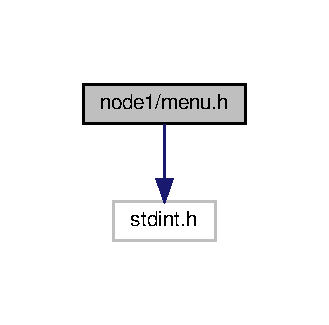
\includegraphics[width=158pt]{menu_8h__incl}
\end{center}
\end{figure}
This graph shows which files directly or indirectly include this file\+:\nopagebreak
\begin{figure}[H]
\begin{center}
\leavevmode
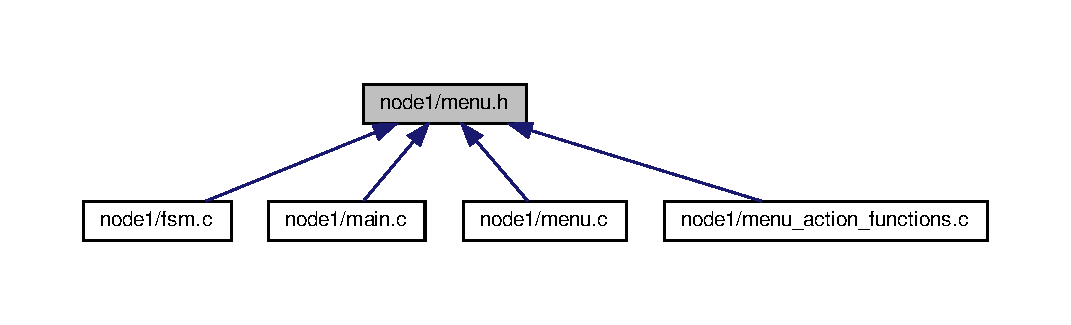
\includegraphics[width=350pt]{menu_8h__dep__incl}
\end{center}
\end{figure}
\subsection*{Data Structures}
\begin{DoxyCompactItemize}
\item 
struct \hyperlink{structmenu}{menu}
\begin{DoxyCompactList}\small\item\em Data structure to represent a menu. Points to the text display of the menu, and menus above and below in the structure. Also points to an array of functions to be called when the option is selected. \end{DoxyCompactList}\end{DoxyCompactItemize}
\subsection*{Macros}
\begin{DoxyCompactItemize}
\item 
\mbox{\Hypertarget{menu_8h_a1b978a465ff0398eaea898634ce9d9b0}\label{menu_8h_a1b978a465ff0398eaea898634ce9d9b0}} 
\#define {\bfseries M\+A\+X\+\_\+\+S\+U\+B\+M\+E\+N\+U\+\_\+\+N\+U\+M\+B\+ER}~5
\end{DoxyCompactItemize}
\subsection*{Typedefs}
\begin{DoxyCompactItemize}
\item 
\mbox{\Hypertarget{menu_8h_aef883fcbc0fedc43ffe831f59194dc5b}\label{menu_8h_aef883fcbc0fedc43ffe831f59194dc5b}} 
typedef struct \hyperlink{structmenu}{menu} \hyperlink{menu_8h_aef883fcbc0fedc43ffe831f59194dc5b}{M\+E\+NU}
\begin{DoxyCompactList}\small\item\em Data structure to represent a menu. Points to the text display of the menu, and menus above and below in the structure. Also points to an array of functions to be called when the option is selected. \end{DoxyCompactList}\end{DoxyCompactItemize}
\subsection*{Functions}
\begin{DoxyCompactItemize}
\item 
\mbox{\Hypertarget{menu_8h_a825deebad1aa530657673fb8a95a2565}\label{menu_8h_a825deebad1aa530657673fb8a95a2565}} 
void \hyperlink{menu_8h_a825deebad1aa530657673fb8a95a2565}{menu\+\_\+init} ()
\begin{DoxyCompactList}\small\item\em Initiates the menu by creating all submenus, with their respective linked lists of nodes. Clears the O\+L\+ED screen and writes the main menu to the S\+R\+AM. \end{DoxyCompactList}\item 
\mbox{\Hypertarget{menu_8h_a0bf8d4a91e08200bd9e1080ad4fd59ae}\label{menu_8h_a0bf8d4a91e08200bd9e1080ad4fd59ae}} 
void \hyperlink{menu_8h_a0bf8d4a91e08200bd9e1080ad4fd59ae}{menu\+\_\+run} ()
\begin{DoxyCompactList}\small\item\em Navigates the menu, depending on the joystick direction. \end{DoxyCompactList}\item 
\mbox{\Hypertarget{menu_8h_a666d48b65f316427066fd81a423ccacc}\label{menu_8h_a666d48b65f316427066fd81a423ccacc}} 
void \hyperlink{menu_8h_a666d48b65f316427066fd81a423ccacc}{menu\+\_\+timer\+\_\+enable} ()
\begin{DoxyCompactList}\small\item\em Enables the timer which prints the menu to the O\+L\+ED screen. \end{DoxyCompactList}\item 
\mbox{\Hypertarget{menu_8h_af317d740a77d0eae48cbe8e2d0d448e9}\label{menu_8h_af317d740a77d0eae48cbe8e2d0d448e9}} 
void \hyperlink{menu_8h_af317d740a77d0eae48cbe8e2d0d448e9}{menu\+\_\+timer\+\_\+disable} ()
\begin{DoxyCompactList}\small\item\em Disables the timer which prints the menu to the O\+L\+ED screen. \end{DoxyCompactList}\item 
\mbox{\Hypertarget{menu_8h_ad14250594b184a816ab6291c37e28809}\label{menu_8h_ad14250594b184a816ab6291c37e28809}} 
void \hyperlink{menu_8h_ad14250594b184a816ab6291c37e28809}{menu\+\_\+go\+\_\+to\+\_\+parent} ()
\begin{DoxyCompactList}\small\item\em Navigates to the menu above the current menu. \end{DoxyCompactList}\item 
\mbox{\Hypertarget{menu_8h_ab6cf37eeeacee3bc68744eaffde1d7d1}\label{menu_8h_ab6cf37eeeacee3bc68744eaffde1d7d1}} 
void \hyperlink{menu_8h_ab6cf37eeeacee3bc68744eaffde1d7d1}{menu\+\_\+go\+\_\+to\+\_\+child} ()
\begin{DoxyCompactList}\small\item\em Navigates to the submenu below the current menu. \end{DoxyCompactList}\end{DoxyCompactItemize}


\subsection{Detailed Description}
Module for the menu system. 


\hypertarget{menu__action__functions_8h}{}\section{node1/menu\+\_\+action\+\_\+functions.h File Reference}
\label{menu__action__functions_8h}\index{node1/menu\+\_\+action\+\_\+functions.\+h@{node1/menu\+\_\+action\+\_\+functions.\+h}}


Module with action functions to be called in the menu system.  


This graph shows which files directly or indirectly include this file\+:\nopagebreak
\begin{figure}[H]
\begin{center}
\leavevmode
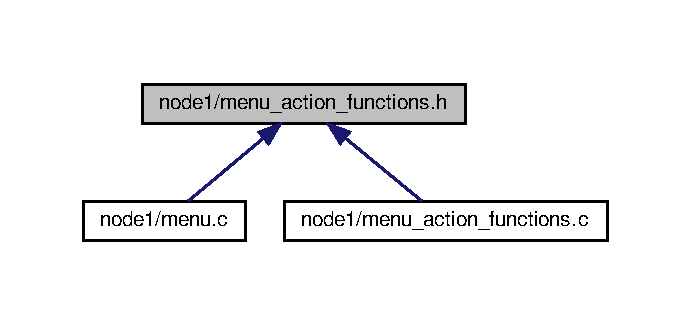
\includegraphics[width=332pt]{menu__action__functions_8h__dep__incl}
\end{center}
\end{figure}
\subsection*{Functions}
\begin{DoxyCompactItemize}
\item 
\mbox{\Hypertarget{menu__action__functions_8h_a43568102f9b3a25a30a1472f9ed03dac}\label{menu__action__functions_8h_a43568102f9b3a25a30a1472f9ed03dac}} 
void \hyperlink{menu__action__functions_8h_a43568102f9b3a25a30a1472f9ed03dac}{start\+\_\+new\+\_\+game} ()
\begin{DoxyCompactList}\small\item\em Starts a new game by transitioning the F\+SM to state P\+L\+A\+Y\+I\+NG. \end{DoxyCompactList}\item 
\mbox{\Hypertarget{menu__action__functions_8h_a519153e39bed47f218143106806429f5}\label{menu__action__functions_8h_a519153e39bed47f218143106806429f5}} 
void \hyperlink{menu__action__functions_8h_a519153e39bed47f218143106806429f5}{select\+\_\+controller\+\_\+slider} ()
\begin{DoxyCompactList}\small\item\em Selects the slider position controller. \end{DoxyCompactList}\item 
\mbox{\Hypertarget{menu__action__functions_8h_ab25d1cab8361209b4df88389231d6610}\label{menu__action__functions_8h_ab25d1cab8361209b4df88389231d6610}} 
void \hyperlink{menu__action__functions_8h_ab25d1cab8361209b4df88389231d6610}{select\+\_\+controller\+\_\+joystick} ()
\begin{DoxyCompactList}\small\item\em Selects the joystick speed controller. \end{DoxyCompactList}\item 
\mbox{\Hypertarget{menu__action__functions_8h_a22f50e95613825410e484c25a8a1c495}\label{menu__action__functions_8h_a22f50e95613825410e484c25a8a1c495}} 
void \hyperlink{menu__action__functions_8h_a22f50e95613825410e484c25a8a1c495}{select\+\_\+controller\+\_\+microbit} ()
\begin{DoxyCompactList}\small\item\em Selects the microbit speed controller. \end{DoxyCompactList}\item 
\mbox{\Hypertarget{menu__action__functions_8h_ac15f962f213f0fe5c10538f1f5c67f05}\label{menu__action__functions_8h_ac15f962f213f0fe5c10538f1f5c67f05}} 
void \hyperlink{menu__action__functions_8h_ac15f962f213f0fe5c10538f1f5c67f05}{set\+\_\+high\+\_\+oled\+\_\+brightness} ()
\begin{DoxyCompactList}\small\item\em Sets the O\+L\+ED screen brightness to high. \end{DoxyCompactList}\item 
\mbox{\Hypertarget{menu__action__functions_8h_ac645e6ae712e4af109615f31802a9944}\label{menu__action__functions_8h_ac645e6ae712e4af109615f31802a9944}} 
void \hyperlink{menu__action__functions_8h_ac645e6ae712e4af109615f31802a9944}{set\+\_\+medium\+\_\+oled\+\_\+brightness} ()
\begin{DoxyCompactList}\small\item\em Sets the O\+L\+ED screen brightness to medium. \end{DoxyCompactList}\item 
\mbox{\Hypertarget{menu__action__functions_8h_ab53ee20410a8ab5dc0f67c9de10205fc}\label{menu__action__functions_8h_ab53ee20410a8ab5dc0f67c9de10205fc}} 
void \hyperlink{menu__action__functions_8h_ab53ee20410a8ab5dc0f67c9de10205fc}{set\+\_\+low\+\_\+oled\+\_\+brightness} ()
\begin{DoxyCompactList}\small\item\em Sets the O\+L\+ED screen brightness to low. \end{DoxyCompactList}\item 
\mbox{\Hypertarget{menu__action__functions_8h_a1cb3ba34a8372c1a13f770b9c0089fbb}\label{menu__action__functions_8h_a1cb3ba34a8372c1a13f770b9c0089fbb}} 
void \hyperlink{menu__action__functions_8h_a1cb3ba34a8372c1a13f770b9c0089fbb}{select\+\_\+song\+\_\+mii\+\_\+theme} ()
\begin{DoxyCompactList}\small\item\em Plays the song \char`\"{}\+Mii Theme\char`\"{}. \end{DoxyCompactList}\item 
\mbox{\Hypertarget{menu__action__functions_8h_afc20b90dbd94cce884c78e27cedfb6a8}\label{menu__action__functions_8h_afc20b90dbd94cce884c78e27cedfb6a8}} 
void \hyperlink{menu__action__functions_8h_afc20b90dbd94cce884c78e27cedfb6a8}{select\+\_\+song\+\_\+mario} ()
\begin{DoxyCompactList}\small\item\em Plays the song \char`\"{}\+Super Mario Bros Theme\char`\"{}. \end{DoxyCompactList}\item 
\mbox{\Hypertarget{menu__action__functions_8h_aea0b4e258901874e54da7050afcd5b03}\label{menu__action__functions_8h_aea0b4e258901874e54da7050afcd5b03}} 
void \hyperlink{menu__action__functions_8h_aea0b4e258901874e54da7050afcd5b03}{select\+\_\+song\+\_\+harry\+\_\+potter} ()
\begin{DoxyCompactList}\small\item\em Plays the song \char`\"{}\+Hedwigs Theme\char`\"{} from Harry Potter. \end{DoxyCompactList}\item 
\mbox{\Hypertarget{menu__action__functions_8h_a75b819df3ebcef53ff9b776fe2594568}\label{menu__action__functions_8h_a75b819df3ebcef53ff9b776fe2594568}} 
void \hyperlink{menu__action__functions_8h_a75b819df3ebcef53ff9b776fe2594568}{select\+\_\+song\+\_\+savage\+\_\+love} ()
\begin{DoxyCompactList}\small\item\em Plays the song \char`\"{}\+Savage Love\char`\"{}. \end{DoxyCompactList}\item 
\mbox{\Hypertarget{menu__action__functions_8h_a3ce6129e7ea65b8a896668d110fae950}\label{menu__action__functions_8h_a3ce6129e7ea65b8a896668d110fae950}} 
void \hyperlink{menu__action__functions_8h_a3ce6129e7ea65b8a896668d110fae950}{stop\+\_\+music} ()
\begin{DoxyCompactList}\small\item\em Stops any playing music and returns to the main menu. \end{DoxyCompactList}\item 
\mbox{\Hypertarget{menu__action__functions_8h_acac297fa7ff2840ff6958bd5686fcec8}\label{menu__action__functions_8h_acac297fa7ff2840ff6958bd5686fcec8}} 
void \hyperlink{menu__action__functions_8h_acac297fa7ff2840ff6958bd5686fcec8}{set\+\_\+difficulty\+\_\+hard} ()
\begin{DoxyCompactList}\small\item\em Sets the game difficulty to hard. \end{DoxyCompactList}\item 
\mbox{\Hypertarget{menu__action__functions_8h_aa2202134252192422511df79fb348b23}\label{menu__action__functions_8h_aa2202134252192422511df79fb348b23}} 
void \hyperlink{menu__action__functions_8h_aa2202134252192422511df79fb348b23}{set\+\_\+difficulty\+\_\+extreme} ()
\begin{DoxyCompactList}\small\item\em Sets the game difficulty to extreme. \end{DoxyCompactList}\item 
\mbox{\Hypertarget{menu__action__functions_8h_a3060fb540c429af0e5d126bb1337f7b8}\label{menu__action__functions_8h_a3060fb540c429af0e5d126bb1337f7b8}} 
void \hyperlink{menu__action__functions_8h_a3060fb540c429af0e5d126bb1337f7b8}{set\+\_\+difficulty\+\_\+impossible} ()
\begin{DoxyCompactList}\small\item\em Sets the game difficulty to impossible. \end{DoxyCompactList}\end{DoxyCompactItemize}


\subsection{Detailed Description}
Module with action functions to be called in the menu system. 


\hypertarget{oled_8h}{}\section{node1/oled.h File Reference}
\label{oled_8h}\index{node1/oled.\+h@{node1/oled.\+h}}


Module for controlling and printing to the O\+L\+ED screen.  


{\ttfamily \#include $<$stdint.\+h$>$}\newline
Include dependency graph for oled.\+h\+:\nopagebreak
\begin{figure}[H]
\begin{center}
\leavevmode
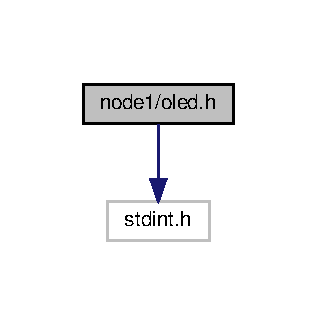
\includegraphics[width=152pt]{oled_8h__incl}
\end{center}
\end{figure}
This graph shows which files directly or indirectly include this file\+:\nopagebreak
\begin{figure}[H]
\begin{center}
\leavevmode
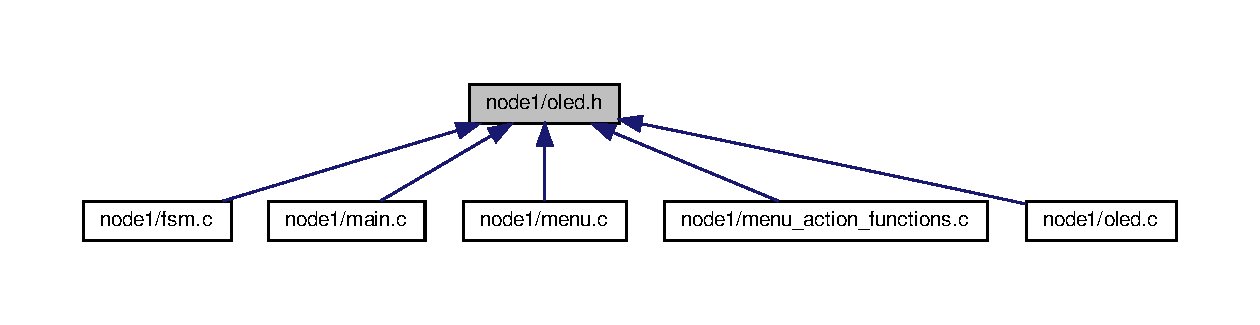
\includegraphics[width=350pt]{oled_8h__dep__incl}
\end{center}
\end{figure}
\subsection*{Macros}
\begin{DoxyCompactItemize}
\item 
\mbox{\Hypertarget{oled_8h_abc4336b9de8d9284f7ade60b4b5d652f}\label{oled_8h_abc4336b9de8d9284f7ade60b4b5d652f}} 
\#define {\bfseries N\+U\+M\+B\+E\+R\+\_\+\+O\+F\+\_\+\+P\+A\+G\+ES}~8
\item 
\mbox{\Hypertarget{oled_8h_a0240364487a54a70da4ffb51459ada98}\label{oled_8h_a0240364487a54a70da4ffb51459ada98}} 
\#define {\bfseries N\+U\+M\+B\+E\+R\+\_\+\+O\+F\+\_\+\+C\+O\+L\+U\+M\+NS}~128
\item 
\mbox{\Hypertarget{oled_8h_ae3c47801ea3ac450ff9b877b1e008e1a}\label{oled_8h_ae3c47801ea3ac450ff9b877b1e008e1a}} 
\#define {\bfseries A\+S\+C\+I\+I\+\_\+\+O\+F\+F\+S\+ET}~32
\item 
\mbox{\Hypertarget{oled_8h_ae06dc7b9804bb102859f0e32754e79a5}\label{oled_8h_ae06dc7b9804bb102859f0e32754e79a5}} 
\#define {\bfseries F\+O\+N\+T\+\_\+\+L\+E\+N\+G\+TH}~8
\end{DoxyCompactItemize}
\subsection*{Functions}
\begin{DoxyCompactItemize}
\item 
\mbox{\Hypertarget{oled_8h_a8c50659733df2acac1580d209db8e97f}\label{oled_8h_a8c50659733df2acac1580d209db8e97f}} 
void \hyperlink{oled_8h_a8c50659733df2acac1580d209db8e97f}{oled\+\_\+init} ()
\begin{DoxyCompactList}\small\item\em Initiates the O\+L\+ED, and clears the screen using {\ttfamily \hyperlink{oled_8h_a66cdd05fb3a765535af54825cb9eb26c}{oled\+\_\+clear()}}. \end{DoxyCompactList}\item 
void \hyperlink{oled_8h_a33f0de77a99d6143e4ccb2baf21e699a}{oled\+\_\+go\+\_\+to\+\_\+line} (int line)
\begin{DoxyCompactList}\small\item\em Updates the O\+L\+ED page pointer. Does nothing if {\ttfamily line} is outside the interval \mbox{[}0,7\mbox{]}. \end{DoxyCompactList}\item 
void \hyperlink{oled_8h_a39da12164c8ef722d0e9f88b1950212a}{oled\+\_\+go\+\_\+to\+\_\+col} (int col)
\begin{DoxyCompactList}\small\item\em Updates the O\+L\+ED column pointer. Does nothing if {\ttfamily line} is outside the interval \mbox{[}0,127\mbox{]}. \end{DoxyCompactList}\item 
void \hyperlink{oled_8h_a3447f323dab2790a195dc636eb97c8b7}{oled\+\_\+set\+\_\+pos} (int line, int col)
\begin{DoxyCompactList}\small\item\em Updates the position pointed to by the page og column poiniters, by using {\ttfamily \hyperlink{oled_8h_a33f0de77a99d6143e4ccb2baf21e699a}{oled\+\_\+go\+\_\+to\+\_\+line()}} and {\ttfamily \hyperlink{oled_8h_a39da12164c8ef722d0e9f88b1950212a}{oled\+\_\+go\+\_\+to\+\_\+col()}}. \end{DoxyCompactList}\item 
\mbox{\Hypertarget{oled_8h_a66cdd05fb3a765535af54825cb9eb26c}\label{oled_8h_a66cdd05fb3a765535af54825cb9eb26c}} 
void \hyperlink{oled_8h_a66cdd05fb3a765535af54825cb9eb26c}{oled\+\_\+clear} (void)
\begin{DoxyCompactList}\small\item\em Clears the O\+L\+ED screen. \end{DoxyCompactList}\item 
void \hyperlink{oled_8h_ab558b8bab1b1f6bc8d573c230cbc20aa}{oled\+\_\+print\+\_\+char} (char c)
\begin{DoxyCompactList}\small\item\em Prints a character {\ttfamily c} to the O\+L\+ED screen in the position pointed to by the page and column pointers. Uses the large font given in {\ttfamily \hyperlink{fonts_8h}{fonts.\+h}}. \end{DoxyCompactList}\item 
void \hyperlink{oled_8h_a47fbb0bd7f8f0a0aac3e90aa49833b69}{oled\+\_\+print\+\_\+string} (const char $\ast$string)
\begin{DoxyCompactList}\small\item\em Prints a character {\ttfamily string} to the O\+L\+ED screen in the position pointed to by the page and column pointers, by using {\ttfamily \hyperlink{oled_8h_ab558b8bab1b1f6bc8d573c230cbc20aa}{oled\+\_\+print\+\_\+char()}}. \end{DoxyCompactList}\item 
void \hyperlink{oled_8h_a3e2dd8ae1ab72c11cd8194407a1d4c5d}{oled\+\_\+print\+\_\+int} (uint16\+\_\+t number)
\begin{DoxyCompactList}\small\item\em Prints an integer {\ttfamily number} to the O\+L\+ED screen in the position pointed to by the page and column pointers, by using {\ttfamily \hyperlink{oled_8h_a47fbb0bd7f8f0a0aac3e90aa49833b69}{oled\+\_\+print\+\_\+string()}}. \end{DoxyCompactList}\item 
void \hyperlink{oled_8h_a6595d2dea96975e71d5a9eb76a9b756f}{oled\+\_\+print\+\_\+playing\+\_\+screen} (int lives\+\_\+left, int max\+\_\+lives)
\begin{DoxyCompactList}\small\item\em Prints the playing screen, showing lives left as filled hearts, and lives lost as empty hearts. \end{DoxyCompactList}\item 
\mbox{\Hypertarget{oled_8h_a4c5b25604dfc14447301e518966f9b62}\label{oled_8h_a4c5b25604dfc14447301e518966f9b62}} 
void \hyperlink{oled_8h_a4c5b25604dfc14447301e518966f9b62}{oled\+\_\+print\+\_\+quit\+\_\+screen} (void)
\begin{DoxyCompactList}\small\item\em Prints the quit screen. \end{DoxyCompactList}\item 
void \hyperlink{oled_8h_a1802dd010241b5549bf382e441480457}{oled\+\_\+print\+\_\+game\+\_\+over\+\_\+screen} (int score, char new\+\_\+highscore)
\begin{DoxyCompactList}\small\item\em Prints the game over screen, which displays {\ttfamily score}. \end{DoxyCompactList}\item 
\mbox{\Hypertarget{oled_8h_ac621da3bb2f74172c96e297ad0f8e642}\label{oled_8h_ac621da3bb2f74172c96e297ad0f8e642}} 
void \hyperlink{oled_8h_ac621da3bb2f74172c96e297ad0f8e642}{oled\+\_\+print\+\_\+from\+\_\+sram} ()
\begin{DoxyCompactList}\small\item\em Prints the first 1024 bytes of the S\+R\+AM memory to the O\+L\+ED screen. \end{DoxyCompactList}\item 
void \hyperlink{oled_8h_a75681f1038002d7d3ea4fe0ad379c715}{oled\+\_\+set\+\_\+brightness} (uint8\+\_\+t brightness)
\begin{DoxyCompactList}\small\item\em Adjusts the brightness of the O\+L\+ED screen. \end{DoxyCompactList}\end{DoxyCompactItemize}


\subsection{Detailed Description}
Module for controlling and printing to the O\+L\+ED screen. 



\subsection{Function Documentation}
\mbox{\Hypertarget{oled_8h_a39da12164c8ef722d0e9f88b1950212a}\label{oled_8h_a39da12164c8ef722d0e9f88b1950212a}} 
\index{oled.\+h@{oled.\+h}!oled\+\_\+go\+\_\+to\+\_\+col@{oled\+\_\+go\+\_\+to\+\_\+col}}
\index{oled\+\_\+go\+\_\+to\+\_\+col@{oled\+\_\+go\+\_\+to\+\_\+col}!oled.\+h@{oled.\+h}}
\subsubsection{\texorpdfstring{oled\+\_\+go\+\_\+to\+\_\+col()}{oled\_go\_to\_col()}}
{\footnotesize\ttfamily void oled\+\_\+go\+\_\+to\+\_\+col (\begin{DoxyParamCaption}\item[{int}]{col }\end{DoxyParamCaption})}



Updates the O\+L\+ED column pointer. Does nothing if {\ttfamily line} is outside the interval \mbox{[}0,127\mbox{]}. 


\begin{DoxyParams}{Parameters}
{\em col} & New value of the O\+L\+ED column pointer. \\
\hline
\end{DoxyParams}


Definition at line 52 of file oled.\+c.

\mbox{\Hypertarget{oled_8h_a33f0de77a99d6143e4ccb2baf21e699a}\label{oled_8h_a33f0de77a99d6143e4ccb2baf21e699a}} 
\index{oled.\+h@{oled.\+h}!oled\+\_\+go\+\_\+to\+\_\+line@{oled\+\_\+go\+\_\+to\+\_\+line}}
\index{oled\+\_\+go\+\_\+to\+\_\+line@{oled\+\_\+go\+\_\+to\+\_\+line}!oled.\+h@{oled.\+h}}
\subsubsection{\texorpdfstring{oled\+\_\+go\+\_\+to\+\_\+line()}{oled\_go\_to\_line()}}
{\footnotesize\ttfamily void oled\+\_\+go\+\_\+to\+\_\+line (\begin{DoxyParamCaption}\item[{int}]{line }\end{DoxyParamCaption})}



Updates the O\+L\+ED page pointer. Does nothing if {\ttfamily line} is outside the interval \mbox{[}0,7\mbox{]}. 


\begin{DoxyParams}{Parameters}
{\em line} & New value of the O\+L\+ED page pointer. \\
\hline
\end{DoxyParams}


Definition at line 45 of file oled.\+c.

\mbox{\Hypertarget{oled_8h_ab558b8bab1b1f6bc8d573c230cbc20aa}\label{oled_8h_ab558b8bab1b1f6bc8d573c230cbc20aa}} 
\index{oled.\+h@{oled.\+h}!oled\+\_\+print\+\_\+char@{oled\+\_\+print\+\_\+char}}
\index{oled\+\_\+print\+\_\+char@{oled\+\_\+print\+\_\+char}!oled.\+h@{oled.\+h}}
\subsubsection{\texorpdfstring{oled\+\_\+print\+\_\+char()}{oled\_print\_char()}}
{\footnotesize\ttfamily void oled\+\_\+print\+\_\+char (\begin{DoxyParamCaption}\item[{char}]{c }\end{DoxyParamCaption})}



Prints a character {\ttfamily c} to the O\+L\+ED screen in the position pointed to by the page and column pointers. Uses the large font given in {\ttfamily \hyperlink{fonts_8h}{fonts.\+h}}. 


\begin{DoxyParams}{Parameters}
{\em c} & Character to be printed to the O\+L\+ED screen. \\
\hline
\end{DoxyParams}


Definition at line 79 of file oled.\+c.

\mbox{\Hypertarget{oled_8h_a1802dd010241b5549bf382e441480457}\label{oled_8h_a1802dd010241b5549bf382e441480457}} 
\index{oled.\+h@{oled.\+h}!oled\+\_\+print\+\_\+game\+\_\+over\+\_\+screen@{oled\+\_\+print\+\_\+game\+\_\+over\+\_\+screen}}
\index{oled\+\_\+print\+\_\+game\+\_\+over\+\_\+screen@{oled\+\_\+print\+\_\+game\+\_\+over\+\_\+screen}!oled.\+h@{oled.\+h}}
\subsubsection{\texorpdfstring{oled\+\_\+print\+\_\+game\+\_\+over\+\_\+screen()}{oled\_print\_game\_over\_screen()}}
{\footnotesize\ttfamily void oled\+\_\+print\+\_\+game\+\_\+over\+\_\+screen (\begin{DoxyParamCaption}\item[{int}]{score,  }\item[{char}]{new\+\_\+highscore }\end{DoxyParamCaption})}



Prints the game over screen, which displays {\ttfamily score}. 


\begin{DoxyParams}{Parameters}
{\em score} & Score to be displayed. \\
\hline
{\em new\+\_\+highscore} & If 1, player is congratulated with achieving a new highscore. \\
\hline
\end{DoxyParams}


Definition at line 171 of file oled.\+c.

\mbox{\Hypertarget{oled_8h_a3e2dd8ae1ab72c11cd8194407a1d4c5d}\label{oled_8h_a3e2dd8ae1ab72c11cd8194407a1d4c5d}} 
\index{oled.\+h@{oled.\+h}!oled\+\_\+print\+\_\+int@{oled\+\_\+print\+\_\+int}}
\index{oled\+\_\+print\+\_\+int@{oled\+\_\+print\+\_\+int}!oled.\+h@{oled.\+h}}
\subsubsection{\texorpdfstring{oled\+\_\+print\+\_\+int()}{oled\_print\_int()}}
{\footnotesize\ttfamily void oled\+\_\+print\+\_\+int (\begin{DoxyParamCaption}\item[{uint16\+\_\+t}]{number }\end{DoxyParamCaption})}



Prints an integer {\ttfamily number} to the O\+L\+ED screen in the position pointed to by the page and column pointers, by using {\ttfamily \hyperlink{oled_8h_a47fbb0bd7f8f0a0aac3e90aa49833b69}{oled\+\_\+print\+\_\+string()}}. 


\begin{DoxyParams}{Parameters}
{\em number} & Integer to be printed to the O\+L\+ED screen. \\
\hline
\end{DoxyParams}


Definition at line 98 of file oled.\+c.

\mbox{\Hypertarget{oled_8h_a6595d2dea96975e71d5a9eb76a9b756f}\label{oled_8h_a6595d2dea96975e71d5a9eb76a9b756f}} 
\index{oled.\+h@{oled.\+h}!oled\+\_\+print\+\_\+playing\+\_\+screen@{oled\+\_\+print\+\_\+playing\+\_\+screen}}
\index{oled\+\_\+print\+\_\+playing\+\_\+screen@{oled\+\_\+print\+\_\+playing\+\_\+screen}!oled.\+h@{oled.\+h}}
\subsubsection{\texorpdfstring{oled\+\_\+print\+\_\+playing\+\_\+screen()}{oled\_print\_playing\_screen()}}
{\footnotesize\ttfamily void oled\+\_\+print\+\_\+playing\+\_\+screen (\begin{DoxyParamCaption}\item[{int}]{lives\+\_\+left,  }\item[{int}]{max\+\_\+lives }\end{DoxyParamCaption})}



Prints the playing screen, showing lives left as filled hearts, and lives lost as empty hearts. 


\begin{DoxyParams}{Parameters}
{\em lives\+\_\+left} & Amount of filled hearts. \\
\hline
{\em max\+\_\+lives} & Number of hearts on screen. \\
\hline
\end{DoxyParams}


Definition at line 143 of file oled.\+c.

\mbox{\Hypertarget{oled_8h_a47fbb0bd7f8f0a0aac3e90aa49833b69}\label{oled_8h_a47fbb0bd7f8f0a0aac3e90aa49833b69}} 
\index{oled.\+h@{oled.\+h}!oled\+\_\+print\+\_\+string@{oled\+\_\+print\+\_\+string}}
\index{oled\+\_\+print\+\_\+string@{oled\+\_\+print\+\_\+string}!oled.\+h@{oled.\+h}}
\subsubsection{\texorpdfstring{oled\+\_\+print\+\_\+string()}{oled\_print\_string()}}
{\footnotesize\ttfamily void oled\+\_\+print\+\_\+string (\begin{DoxyParamCaption}\item[{const char $\ast$}]{string }\end{DoxyParamCaption})}



Prints a character {\ttfamily string} to the O\+L\+ED screen in the position pointed to by the page and column pointers, by using {\ttfamily \hyperlink{oled_8h_ab558b8bab1b1f6bc8d573c230cbc20aa}{oled\+\_\+print\+\_\+char()}}. 


\begin{DoxyParams}{Parameters}
{\em string} & String to be printed to the O\+L\+ED screen. \\
\hline
\end{DoxyParams}


Definition at line 89 of file oled.\+c.

\mbox{\Hypertarget{oled_8h_a75681f1038002d7d3ea4fe0ad379c715}\label{oled_8h_a75681f1038002d7d3ea4fe0ad379c715}} 
\index{oled.\+h@{oled.\+h}!oled\+\_\+set\+\_\+brightness@{oled\+\_\+set\+\_\+brightness}}
\index{oled\+\_\+set\+\_\+brightness@{oled\+\_\+set\+\_\+brightness}!oled.\+h@{oled.\+h}}
\subsubsection{\texorpdfstring{oled\+\_\+set\+\_\+brightness()}{oled\_set\_brightness()}}
{\footnotesize\ttfamily void oled\+\_\+set\+\_\+brightness (\begin{DoxyParamCaption}\item[{uint8\+\_\+t}]{brightness }\end{DoxyParamCaption})}



Adjusts the brightness of the O\+L\+ED screen. 


\begin{DoxyParams}{Parameters}
{\em brightness} & Desired brightness. \\
\hline
\end{DoxyParams}


Definition at line 205 of file oled.\+c.

\mbox{\Hypertarget{oled_8h_a3447f323dab2790a195dc636eb97c8b7}\label{oled_8h_a3447f323dab2790a195dc636eb97c8b7}} 
\index{oled.\+h@{oled.\+h}!oled\+\_\+set\+\_\+pos@{oled\+\_\+set\+\_\+pos}}
\index{oled\+\_\+set\+\_\+pos@{oled\+\_\+set\+\_\+pos}!oled.\+h@{oled.\+h}}
\subsubsection{\texorpdfstring{oled\+\_\+set\+\_\+pos()}{oled\_set\_pos()}}
{\footnotesize\ttfamily void oled\+\_\+set\+\_\+pos (\begin{DoxyParamCaption}\item[{int}]{line,  }\item[{int}]{col }\end{DoxyParamCaption})}



Updates the position pointed to by the page og column poiniters, by using {\ttfamily \hyperlink{oled_8h_a33f0de77a99d6143e4ccb2baf21e699a}{oled\+\_\+go\+\_\+to\+\_\+line()}} and {\ttfamily \hyperlink{oled_8h_a39da12164c8ef722d0e9f88b1950212a}{oled\+\_\+go\+\_\+to\+\_\+col()}}. 


\begin{DoxyParams}{Parameters}
{\em line} & New value of the O\+L\+ED page pointer. \\
\hline
{\em col} & New value of the O\+L\+ED column pointer. \\
\hline
\end{DoxyParams}


Definition at line 63 of file oled.\+c.


\hypertarget{spi__driver_8h}{}\section{node1/spi\+\_\+driver.h File Reference}
\label{spi__driver_8h}\index{node1/spi\+\_\+driver.\+h@{node1/spi\+\_\+driver.\+h}}


Module for sending and receiving messages over the S\+PI bus.  


{\ttfamily \#include $<$stdint.\+h$>$}\newline
Include dependency graph for spi\+\_\+driver.\+h\+:\nopagebreak
\begin{figure}[H]
\begin{center}
\leavevmode
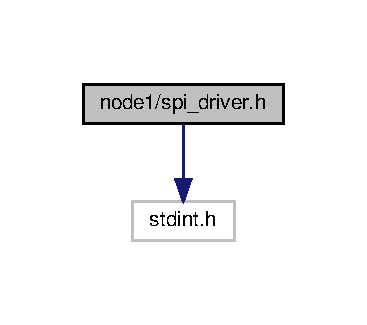
\includegraphics[width=176pt]{spi__driver_8h__incl}
\end{center}
\end{figure}
This graph shows which files directly or indirectly include this file\+:\nopagebreak
\begin{figure}[H]
\begin{center}
\leavevmode
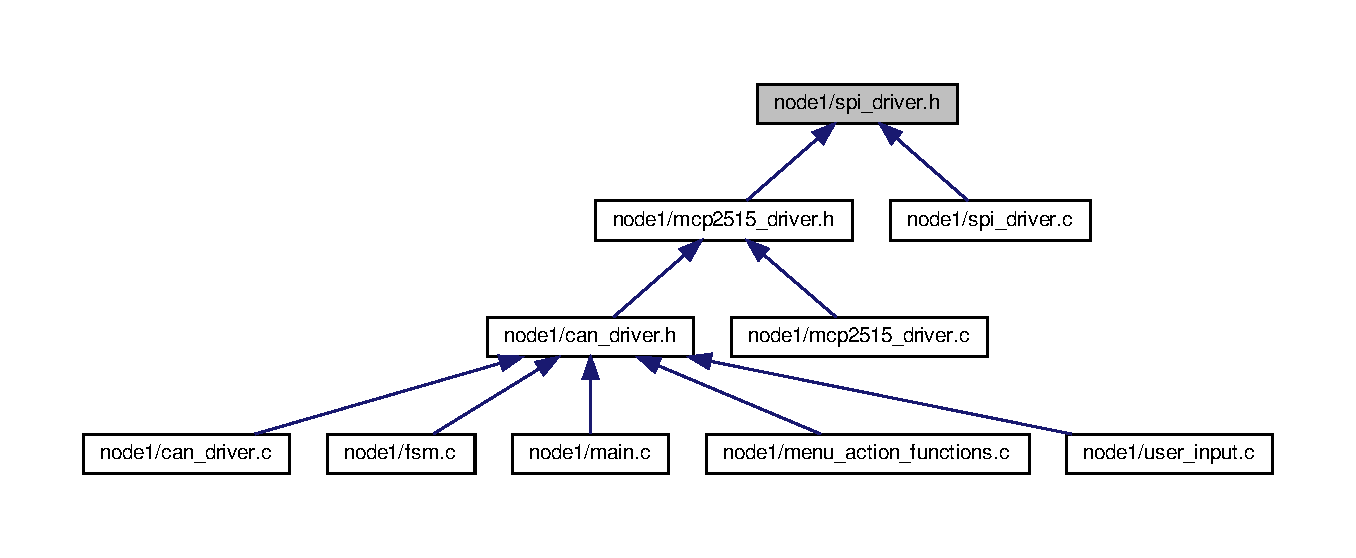
\includegraphics[width=350pt]{spi__driver_8h__dep__incl}
\end{center}
\end{figure}
\subsection*{Functions}
\begin{DoxyCompactItemize}
\item 
\mbox{\Hypertarget{spi__driver_8h_ae909944aa85ae98323073c628be541aa}\label{spi__driver_8h_ae909944aa85ae98323073c628be541aa}} 
void \hyperlink{spi__driver_8h_ae909944aa85ae98323073c628be541aa}{spi\+\_\+init} (void)
\begin{DoxyCompactList}\small\item\em Initiates the S\+PI driver by configuring data directions, and setting the A\+T\+Mega162 to be master node. \end{DoxyCompactList}\item 
void \hyperlink{spi__driver_8h_a49f141469f72b159771fb765a78ecbe5}{spi\+\_\+write} (char data)
\begin{DoxyCompactList}\small\item\em Transmits a data byte to the slave on the S\+PI bus. \end{DoxyCompactList}\item 
\mbox{\Hypertarget{spi__driver_8h_a738951e73ed07d1e0177c8f66964afc3}\label{spi__driver_8h_a738951e73ed07d1e0177c8f66964afc3}} 
uint8\+\_\+t \hyperlink{spi__driver_8h_a738951e73ed07d1e0177c8f66964afc3}{spi\+\_\+read} ()
\begin{DoxyCompactList}\small\item\em Recieves a data byte from the slave the S\+PI bus. \end{DoxyCompactList}\end{DoxyCompactItemize}


\subsection{Detailed Description}
Module for sending and receiving messages over the S\+PI bus. 



\subsection{Function Documentation}
\mbox{\Hypertarget{spi__driver_8h_a49f141469f72b159771fb765a78ecbe5}\label{spi__driver_8h_a49f141469f72b159771fb765a78ecbe5}} 
\index{spi\+\_\+driver.\+h@{spi\+\_\+driver.\+h}!spi\+\_\+write@{spi\+\_\+write}}
\index{spi\+\_\+write@{spi\+\_\+write}!spi\+\_\+driver.\+h@{spi\+\_\+driver.\+h}}
\subsubsection{\texorpdfstring{spi\+\_\+write()}{spi\_write()}}
{\footnotesize\ttfamily void spi\+\_\+write (\begin{DoxyParamCaption}\item[{char}]{data }\end{DoxyParamCaption})}



Transmits a data byte to the slave on the S\+PI bus. 


\begin{DoxyParams}{Parameters}
{\em data} & Byte to be transmitted. \\
\hline
\end{DoxyParams}


Definition at line 18 of file spi\+\_\+driver.\+c.


\hypertarget{sram_8h}{}\section{node1/sram.h File Reference}
\label{sram_8h}\index{node1/sram.\+h@{node1/sram.\+h}}


Module for reading from and writing to the S\+R\+AM.  


{\ttfamily \#include $<$stdint.\+h$>$}\newline
Include dependency graph for sram.\+h\+:\nopagebreak
\begin{figure}[H]
\begin{center}
\leavevmode
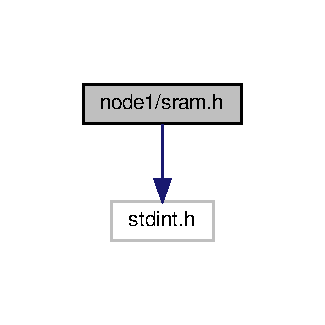
\includegraphics[width=156pt]{sram_8h__incl}
\end{center}
\end{figure}
This graph shows which files directly or indirectly include this file\+:\nopagebreak
\begin{figure}[H]
\begin{center}
\leavevmode
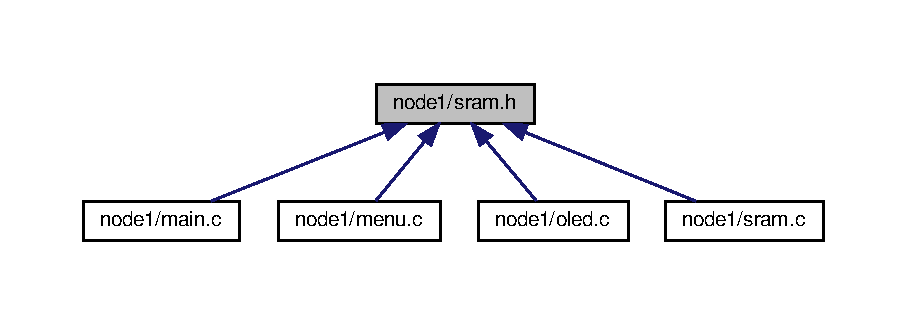
\includegraphics[width=350pt]{sram_8h__dep__incl}
\end{center}
\end{figure}
\subsection*{Functions}
\begin{DoxyCompactItemize}
\item 
\mbox{\Hypertarget{sram_8h_a95a334ecab578f183f77e75f8ab52bbe}\label{sram_8h_a95a334ecab578f183f77e75f8ab52bbe}} 
void \hyperlink{sram_8h_a95a334ecab578f183f77e75f8ab52bbe}{sram\+\_\+init} (void)
\begin{DoxyCompactList}\small\item\em Initiates the external memory by enabling the required pins on the M\+CU. \end{DoxyCompactList}\item 
void \hyperlink{sram_8h_a8fce4e49266a872db4af56b2b02d6b76}{sram\+\_\+write} (uint8\+\_\+t data, uint16\+\_\+t addr)
\begin{DoxyCompactList}\small\item\em Writes {\ttfamily data} to the address {\ttfamily addr}, defined as offset from {\ttfamily 0x1800}. \end{DoxyCompactList}\item 
uint8\+\_\+t \hyperlink{sram_8h_a57e52e7e762b18068fba46a8bf8b7d22}{sram\+\_\+read} (uint16\+\_\+t addr)
\begin{DoxyCompactList}\small\item\em Reads from the address {\ttfamily addr}, defined as offset from {\ttfamily 0x1800}. \end{DoxyCompactList}\item 
\mbox{\Hypertarget{sram_8h_a5398d7c2f04f1096190f6e4bfd75f7b6}\label{sram_8h_a5398d7c2f04f1096190f6e4bfd75f7b6}} 
void \hyperlink{sram_8h_a5398d7c2f04f1096190f6e4bfd75f7b6}{sram\+\_\+test} (void)
\begin{DoxyCompactList}\small\item\em Performs a S\+R\+AM test with random writes and consequent reads. Prints the result using {\ttfamily printf()}. \end{DoxyCompactList}\end{DoxyCompactItemize}


\subsection{Detailed Description}
Module for reading from and writing to the S\+R\+AM. 



\subsection{Function Documentation}
\mbox{\Hypertarget{sram_8h_a57e52e7e762b18068fba46a8bf8b7d22}\label{sram_8h_a57e52e7e762b18068fba46a8bf8b7d22}} 
\index{sram.\+h@{sram.\+h}!sram\+\_\+read@{sram\+\_\+read}}
\index{sram\+\_\+read@{sram\+\_\+read}!sram.\+h@{sram.\+h}}
\subsubsection{\texorpdfstring{sram\+\_\+read()}{sram\_read()}}
{\footnotesize\ttfamily uint8\+\_\+t sram\+\_\+read (\begin{DoxyParamCaption}\item[{uint16\+\_\+t}]{addr }\end{DoxyParamCaption})}



Reads from the address {\ttfamily addr}, defined as offset from {\ttfamily 0x1800}. 


\begin{DoxyParams}{Parameters}
{\em addr} & Offset from the base address {\ttfamily 0x1800} in the external memery address space.\\
\hline
\end{DoxyParams}
\begin{DoxyReturn}{Returns}
The 8-\/bit data at the address given på {\ttfamily addr}. 
\end{DoxyReturn}


Definition at line 22 of file sram.\+c.

\mbox{\Hypertarget{sram_8h_a8fce4e49266a872db4af56b2b02d6b76}\label{sram_8h_a8fce4e49266a872db4af56b2b02d6b76}} 
\index{sram.\+h@{sram.\+h}!sram\+\_\+write@{sram\+\_\+write}}
\index{sram\+\_\+write@{sram\+\_\+write}!sram.\+h@{sram.\+h}}
\subsubsection{\texorpdfstring{sram\+\_\+write()}{sram\_write()}}
{\footnotesize\ttfamily void sram\+\_\+write (\begin{DoxyParamCaption}\item[{uint8\+\_\+t}]{data,  }\item[{uint16\+\_\+t}]{addr }\end{DoxyParamCaption})}



Writes {\ttfamily data} to the address {\ttfamily addr}, defined as offset from {\ttfamily 0x1800}. 


\begin{DoxyParams}{Parameters}
{\em data} & 8-\/bit value to be written to the external memory. \\
\hline
{\em addr} & Offset from the base address {\ttfamily 0x1800} in the external memery address space. \\
\hline
\end{DoxyParams}


Definition at line 16 of file sram.\+c.


\hypertarget{uart_8h}{}\section{node1/uart.h File Reference}
\label{uart_8h}\index{node1/uart.\+h@{node1/uart.\+h}}


Module for sending and receiving messages through the U\+A\+RT.  


This graph shows which files directly or indirectly include this file\+:\nopagebreak
\begin{figure}[H]
\begin{center}
\leavevmode
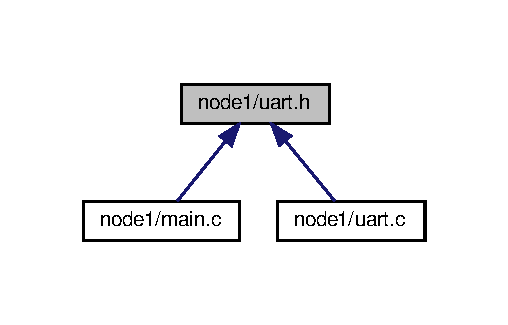
\includegraphics[width=244pt]{uart_8h__dep__incl}
\end{center}
\end{figure}
\subsection*{Functions}
\begin{DoxyCompactItemize}
\item 
void \hyperlink{uart_8h_a6cd2d179b253d22b5cb7d6b97e26a6b2}{uart\+\_\+init} (unsigned int ubrr)
\begin{DoxyCompactList}\small\item\em Initiates the uart module by enabling the necessary registers, and setting baudrate and frame format. \end{DoxyCompactList}\item 
void \hyperlink{uart_8h_ae049828d050821180abb9bedd1af7d0a}{uart\+\_\+transmit} (unsigned char data)
\begin{DoxyCompactList}\small\item\em Tranmits {\ttfamily data} to the M\+CU. \end{DoxyCompactList}\item 
unsigned char \hyperlink{uart_8h_ae29439787a3b89a40ed63c5cac6ad75e}{uart\+\_\+recieve} ()
\begin{DoxyCompactList}\small\item\em Recieves data from the M\+CU. \end{DoxyCompactList}\item 
\mbox{\Hypertarget{uart_8h_a5a3233a1ec3b7fac14ef0a03c1b39bca}\label{uart_8h_a5a3233a1ec3b7fac14ef0a03c1b39bca}} 
void \hyperlink{uart_8h_a5a3233a1ec3b7fac14ef0a03c1b39bca}{uart\+\_\+link\+\_\+printf} ()
\begin{DoxyCompactList}\small\item\em Links the {\ttfamily printf()} function to the uart module. \end{DoxyCompactList}\end{DoxyCompactItemize}


\subsection{Detailed Description}
Module for sending and receiving messages through the U\+A\+RT. 



\subsection{Function Documentation}
\mbox{\Hypertarget{uart_8h_a6cd2d179b253d22b5cb7d6b97e26a6b2}\label{uart_8h_a6cd2d179b253d22b5cb7d6b97e26a6b2}} 
\index{uart.\+h@{uart.\+h}!uart\+\_\+init@{uart\+\_\+init}}
\index{uart\+\_\+init@{uart\+\_\+init}!uart.\+h@{uart.\+h}}
\subsubsection{\texorpdfstring{uart\+\_\+init()}{uart\_init()}}
{\footnotesize\ttfamily void uart\+\_\+init (\begin{DoxyParamCaption}\item[{unsigned int}]{ubrr }\end{DoxyParamCaption})}



Initiates the uart module by enabling the necessary registers, and setting baudrate and frame format. 


\begin{DoxyParams}{Parameters}
{\em ubrr} & Value used to compute baudrate. \\
\hline
\end{DoxyParams}


Definition at line 5 of file uart.\+c.

\mbox{\Hypertarget{uart_8h_ae29439787a3b89a40ed63c5cac6ad75e}\label{uart_8h_ae29439787a3b89a40ed63c5cac6ad75e}} 
\index{uart.\+h@{uart.\+h}!uart\+\_\+recieve@{uart\+\_\+recieve}}
\index{uart\+\_\+recieve@{uart\+\_\+recieve}!uart.\+h@{uart.\+h}}
\subsubsection{\texorpdfstring{uart\+\_\+recieve()}{uart\_recieve()}}
{\footnotesize\ttfamily unsigned char uart\+\_\+recieve (\begin{DoxyParamCaption}{ }\end{DoxyParamCaption})}



Recieves data from the M\+CU. 

\begin{DoxyReturn}{Returns}
8-\/bit value recieved from the M\+CU. 
\end{DoxyReturn}


Definition at line 29 of file uart.\+c.

\mbox{\Hypertarget{uart_8h_ae049828d050821180abb9bedd1af7d0a}\label{uart_8h_ae049828d050821180abb9bedd1af7d0a}} 
\index{uart.\+h@{uart.\+h}!uart\+\_\+transmit@{uart\+\_\+transmit}}
\index{uart\+\_\+transmit@{uart\+\_\+transmit}!uart.\+h@{uart.\+h}}
\subsubsection{\texorpdfstring{uart\+\_\+transmit()}{uart\_transmit()}}
{\footnotesize\ttfamily void uart\+\_\+transmit (\begin{DoxyParamCaption}\item[{unsigned char}]{data }\end{DoxyParamCaption})}



Tranmits {\ttfamily data} to the M\+CU. 


\begin{DoxyParams}{Parameters}
{\em data} & 8-\/bit value to be tranmitted. \\
\hline
\end{DoxyParams}


Definition at line 20 of file uart.\+c.


\hypertarget{node1_2user__input_8h}{}\section{node1/user\+\_\+input.h File Reference}
\label{node1_2user__input_8h}\index{node1/user\+\_\+input.\+h@{node1/user\+\_\+input.\+h}}


Module for reading and transmitting user input data from the U\+SB multifunction board..  


{\ttfamily \#include $<$stdint.\+h$>$}\newline
Include dependency graph for user\+\_\+input.\+h\+:\nopagebreak
\begin{figure}[H]
\begin{center}
\leavevmode
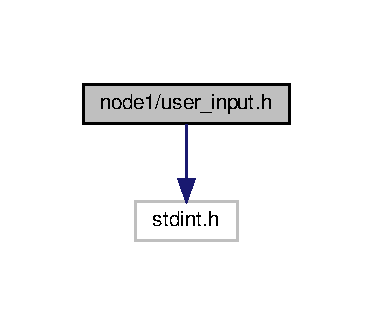
\includegraphics[width=179pt]{node1_2user__input_8h__incl}
\end{center}
\end{figure}
This graph shows which files directly or indirectly include this file\+:\nopagebreak
\begin{figure}[H]
\begin{center}
\leavevmode
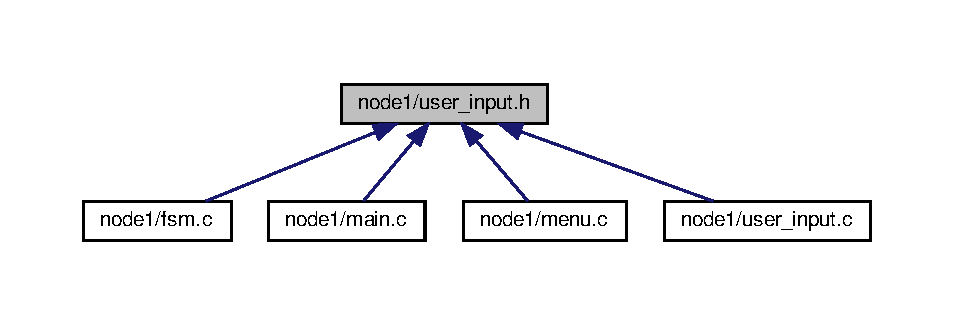
\includegraphics[width=350pt]{node1_2user__input_8h__dep__incl}
\end{center}
\end{figure}
\subsection*{Data Structures}
\begin{DoxyCompactItemize}
\item 
struct \hyperlink{structJOYSTICK__POS}{J\+O\+Y\+S\+T\+I\+C\+K\+\_\+\+P\+OS}
\begin{DoxyCompactList}\small\item\em Data structure to be used to represent the joystick position. \end{DoxyCompactList}\item 
struct \hyperlink{structSLIDER__POS}{S\+L\+I\+D\+E\+R\+\_\+\+P\+OS}
\begin{DoxyCompactList}\small\item\em Data structure to be used to represent the position of the two sliders. \end{DoxyCompactList}\item 
struct \hyperlink{structBUTTONS}{B\+U\+T\+T\+O\+NS}
\begin{DoxyCompactList}\small\item\em Data structure to be used to represent the status of the three buttons. \end{DoxyCompactList}\end{DoxyCompactItemize}
\subsection*{Enumerations}
\begin{DoxyCompactItemize}
\item 
\mbox{\Hypertarget{node1_2user__input_8h_a76b104ee703e253f2bff35f2beee628d}\label{node1_2user__input_8h_a76b104ee703e253f2bff35f2beee628d}} 
enum \hyperlink{node1_2user__input_8h_a76b104ee703e253f2bff35f2beee628d}{J\+O\+Y\+S\+T\+I\+C\+K\+\_\+\+D\+IR} \{ \newline
{\bfseries UP}, 
{\bfseries D\+O\+WN}, 
{\bfseries L\+E\+FT}, 
{\bfseries R\+I\+G\+HT}, 
\newline
{\bfseries C\+E\+N\+T\+ER}, 
{\bfseries N\+E\+U\+T\+R\+AL}
 \}\begin{DoxyCompactList}\small\item\em The different directions the joystick can point. \end{DoxyCompactList}
\end{DoxyCompactItemize}
\subsection*{Functions}
\begin{DoxyCompactItemize}
\item 
\mbox{\Hypertarget{node1_2user__input_8h_ac90157a0f1482f163abc8b24a02907fb}\label{node1_2user__input_8h_ac90157a0f1482f163abc8b24a02907fb}} 
void \hyperlink{node1_2user__input_8h_ac90157a0f1482f163abc8b24a02907fb}{user\+\_\+input\+\_\+init} (void)
\begin{DoxyCompactList}\small\item\em Initiates the user input modeule by initiating the A\+DC, configuring input pins for the button, and setting up a timer for timed transmissions. \end{DoxyCompactList}\item 
\hyperlink{structJOYSTICK__POS}{J\+O\+Y\+S\+T\+I\+C\+K\+\_\+\+P\+OS} \hyperlink{node1_2user__input_8h_a33325461fea91ff023c9f5c1fb7372cf}{user\+\_\+input\+\_\+joystick\+\_\+pos} (void)
\begin{DoxyCompactList}\small\item\em Reads the joystick position through the A\+DC. Returns a position with x and y values in the interval \mbox{[}0, 255\mbox{]}. \end{DoxyCompactList}\item 
\hyperlink{node1_2user__input_8h_a76b104ee703e253f2bff35f2beee628d}{J\+O\+Y\+S\+T\+I\+C\+K\+\_\+\+D\+IR} \hyperlink{node1_2user__input_8h_a2adb6f7e123060a4c81ec9a70b9ef725}{user\+\_\+input\+\_\+joystick\+\_\+dir} (void)
\begin{DoxyCompactList}\small\item\em Calculates the joystick\textquotesingle{}s direction from it\textquotesingle{}s postiton. Reads the joystick position using {\ttfamily joystick\+\_\+pos\+\_\+read()}. \end{DoxyCompactList}\item 
\hyperlink{structSLIDER__POS}{S\+L\+I\+D\+E\+R\+\_\+\+P\+OS} \hyperlink{node1_2user__input_8h_a2bd9ad54baa6f5e04ef577f67ea3579d}{user\+\_\+input\+\_\+slider\+\_\+pos} (void)
\begin{DoxyCompactList}\small\item\em Reads the slider position through the A\+DC. Returns a position for the left and right slider values in the interval \mbox{[}0, 255\mbox{]}. \end{DoxyCompactList}\item 
\hyperlink{structBUTTONS}{B\+U\+T\+T\+O\+NS} \hyperlink{node1_2user__input_8h_a1229ee3a2d02735fb14d044a83781ded}{user\+\_\+input\+\_\+buttons} (void)
\begin{DoxyCompactList}\small\item\em Reads the button statuses. Returns 1 if a button is pressed, and 0 otherwise. \end{DoxyCompactList}\item 
\mbox{\Hypertarget{node1_2user__input_8h_a9451713cb4707bf0bdbb90f32b078eb2}\label{node1_2user__input_8h_a9451713cb4707bf0bdbb90f32b078eb2}} 
void \hyperlink{node1_2user__input_8h_a9451713cb4707bf0bdbb90f32b078eb2}{user\+\_\+input\+\_\+transmit} (void)
\begin{DoxyCompactList}\small\item\em Transmits all the input data over the C\+AN bus. \end{DoxyCompactList}\item 
\mbox{\Hypertarget{node1_2user__input_8h_a9d3099164b85e4f6c6faa63fcbfcad0d}\label{node1_2user__input_8h_a9d3099164b85e4f6c6faa63fcbfcad0d}} 
void \hyperlink{node1_2user__input_8h_a9d3099164b85e4f6c6faa63fcbfcad0d}{user\+\_\+input\+\_\+timer\+\_\+enable} ()
\begin{DoxyCompactList}\small\item\em Enables the timer which calls {\ttfamily \hyperlink{node1_2user__input_8h_a9451713cb4707bf0bdbb90f32b078eb2}{user\+\_\+input\+\_\+transmit()}} at a frequency of 10 Hz. \end{DoxyCompactList}\item 
\mbox{\Hypertarget{node1_2user__input_8h_a0f0406087b958880d329d8a4f07da82a}\label{node1_2user__input_8h_a0f0406087b958880d329d8a4f07da82a}} 
void \hyperlink{node1_2user__input_8h_a0f0406087b958880d329d8a4f07da82a}{user\+\_\+input\+\_\+timer\+\_\+disable} ()
\begin{DoxyCompactList}\small\item\em Disables the timer which calls {\ttfamily \hyperlink{node1_2user__input_8h_a9451713cb4707bf0bdbb90f32b078eb2}{user\+\_\+input\+\_\+transmit()}}. \end{DoxyCompactList}\end{DoxyCompactItemize}


\subsection{Detailed Description}
Module for reading and transmitting user input data from the U\+SB multifunction board.. 



\subsection{Function Documentation}
\mbox{\Hypertarget{node1_2user__input_8h_a1229ee3a2d02735fb14d044a83781ded}\label{node1_2user__input_8h_a1229ee3a2d02735fb14d044a83781ded}} 
\index{node1/user\+\_\+input.\+h@{node1/user\+\_\+input.\+h}!user\+\_\+input\+\_\+buttons@{user\+\_\+input\+\_\+buttons}}
\index{user\+\_\+input\+\_\+buttons@{user\+\_\+input\+\_\+buttons}!node1/user\+\_\+input.\+h@{node1/user\+\_\+input.\+h}}
\subsubsection{\texorpdfstring{user\+\_\+input\+\_\+buttons()}{user\_input\_buttons()}}
{\footnotesize\ttfamily \hyperlink{structBUTTONS}{B\+U\+T\+T\+O\+NS} user\+\_\+input\+\_\+buttons (\begin{DoxyParamCaption}\item[{void}]{ }\end{DoxyParamCaption})}



Reads the button statuses. Returns 1 if a button is pressed, and 0 otherwise. 

\begin{DoxyReturn}{Returns}
The status of the left, right and joystick buttons. 
\end{DoxyReturn}


Definition at line 123 of file user\+\_\+input.\+c.

\mbox{\Hypertarget{node1_2user__input_8h_a2adb6f7e123060a4c81ec9a70b9ef725}\label{node1_2user__input_8h_a2adb6f7e123060a4c81ec9a70b9ef725}} 
\index{node1/user\+\_\+input.\+h@{node1/user\+\_\+input.\+h}!user\+\_\+input\+\_\+joystick\+\_\+dir@{user\+\_\+input\+\_\+joystick\+\_\+dir}}
\index{user\+\_\+input\+\_\+joystick\+\_\+dir@{user\+\_\+input\+\_\+joystick\+\_\+dir}!node1/user\+\_\+input.\+h@{node1/user\+\_\+input.\+h}}
\subsubsection{\texorpdfstring{user\+\_\+input\+\_\+joystick\+\_\+dir()}{user\_input\_joystick\_dir()}}
{\footnotesize\ttfamily \hyperlink{node1_2user__input_8h_a76b104ee703e253f2bff35f2beee628d}{J\+O\+Y\+S\+T\+I\+C\+K\+\_\+\+D\+IR} user\+\_\+input\+\_\+joystick\+\_\+dir (\begin{DoxyParamCaption}\item[{void}]{ }\end{DoxyParamCaption})}



Calculates the joystick\textquotesingle{}s direction from it\textquotesingle{}s postiton. Reads the joystick position using {\ttfamily joystick\+\_\+pos\+\_\+read()}. 

\begin{DoxyReturn}{Returns}
The direction the joystick is pointing. 
\end{DoxyReturn}


Definition at line 83 of file user\+\_\+input.\+c.

\mbox{\Hypertarget{node1_2user__input_8h_a33325461fea91ff023c9f5c1fb7372cf}\label{node1_2user__input_8h_a33325461fea91ff023c9f5c1fb7372cf}} 
\index{node1/user\+\_\+input.\+h@{node1/user\+\_\+input.\+h}!user\+\_\+input\+\_\+joystick\+\_\+pos@{user\+\_\+input\+\_\+joystick\+\_\+pos}}
\index{user\+\_\+input\+\_\+joystick\+\_\+pos@{user\+\_\+input\+\_\+joystick\+\_\+pos}!node1/user\+\_\+input.\+h@{node1/user\+\_\+input.\+h}}
\subsubsection{\texorpdfstring{user\+\_\+input\+\_\+joystick\+\_\+pos()}{user\_input\_joystick\_pos()}}
{\footnotesize\ttfamily \hyperlink{structJOYSTICK__POS}{J\+O\+Y\+S\+T\+I\+C\+K\+\_\+\+P\+OS} user\+\_\+input\+\_\+joystick\+\_\+pos (\begin{DoxyParamCaption}\item[{void}]{ }\end{DoxyParamCaption})}



Reads the joystick position through the A\+DC. Returns a position with x and y values in the interval \mbox{[}0, 255\mbox{]}. 

\begin{DoxyReturn}{Returns}
The joystick position. 
\end{DoxyReturn}


Definition at line 56 of file user\+\_\+input.\+c.

\mbox{\Hypertarget{node1_2user__input_8h_a2bd9ad54baa6f5e04ef577f67ea3579d}\label{node1_2user__input_8h_a2bd9ad54baa6f5e04ef577f67ea3579d}} 
\index{node1/user\+\_\+input.\+h@{node1/user\+\_\+input.\+h}!user\+\_\+input\+\_\+slider\+\_\+pos@{user\+\_\+input\+\_\+slider\+\_\+pos}}
\index{user\+\_\+input\+\_\+slider\+\_\+pos@{user\+\_\+input\+\_\+slider\+\_\+pos}!node1/user\+\_\+input.\+h@{node1/user\+\_\+input.\+h}}
\subsubsection{\texorpdfstring{user\+\_\+input\+\_\+slider\+\_\+pos()}{user\_input\_slider\_pos()}}
{\footnotesize\ttfamily \hyperlink{structSLIDER__POS}{S\+L\+I\+D\+E\+R\+\_\+\+P\+OS} user\+\_\+input\+\_\+slider\+\_\+pos (\begin{DoxyParamCaption}\item[{void}]{ }\end{DoxyParamCaption})}



Reads the slider position through the A\+DC. Returns a position for the left and right slider values in the interval \mbox{[}0, 255\mbox{]}. 

\begin{DoxyReturn}{Returns}
The slider positions. 
\end{DoxyReturn}


Definition at line 114 of file user\+\_\+input.\+c.


\hypertarget{common_2user__input_8h}{}\section{common/user\+\_\+input.h File Reference}
\label{common_2user__input_8h}\index{common/user\+\_\+input.\+h@{common/user\+\_\+input.\+h}}


User input constants common for node 1 and 2.  


This graph shows which files directly or indirectly include this file\+:
\nopagebreak
\begin{figure}[H]
\begin{center}
\leavevmode
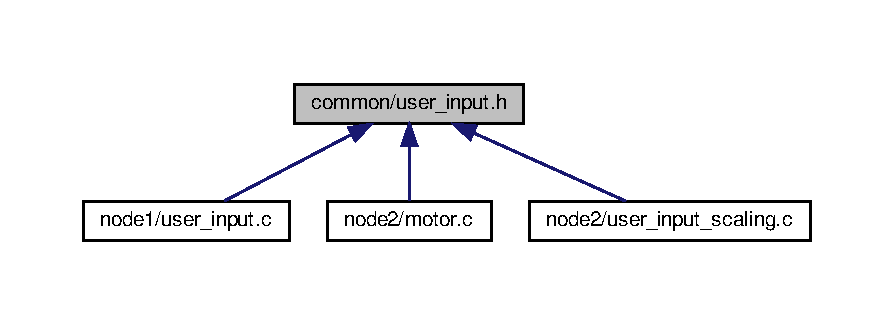
\includegraphics[width=350pt]{common_2user__input_8h__dep__incl}
\end{center}
\end{figure}
\subsection*{Macros}
\begin{DoxyCompactItemize}
\item 
\mbox{\Hypertarget{common_2user__input_8h_a1da18bcf8ecb8711826668136c672c4d}\label{common_2user__input_8h_a1da18bcf8ecb8711826668136c672c4d}} 
\#define {\bfseries J\+O\+Y\+S\+T\+I\+C\+K\+\_\+\+X\+\_\+\+O\+F\+F\+S\+ET}~26
\item 
\mbox{\Hypertarget{common_2user__input_8h_a38f9f58f616c8d416a369930596aee35}\label{common_2user__input_8h_a38f9f58f616c8d416a369930596aee35}} 
\#define {\bfseries J\+O\+Y\+S\+T\+I\+C\+K\+\_\+\+Y\+\_\+\+O\+F\+F\+S\+ET}~28
\item 
\mbox{\Hypertarget{common_2user__input_8h_a7ae7541e97484659ea6bd7a5c63055e5}\label{common_2user__input_8h_a7ae7541e97484659ea6bd7a5c63055e5}} 
\#define {\bfseries J\+O\+Y\+S\+T\+I\+C\+K\+\_\+\+M\+AX}~100
\item 
\mbox{\Hypertarget{common_2user__input_8h_ade60d6c5154f89301e6b09908dc47c59}\label{common_2user__input_8h_ade60d6c5154f89301e6b09908dc47c59}} 
\#define {\bfseries J\+O\+Y\+S\+T\+I\+C\+K\+\_\+\+M\+IN}~-\/100
\item 
\mbox{\Hypertarget{common_2user__input_8h_a3a79356d599df70e735ffe6f2686b6b9}\label{common_2user__input_8h_a3a79356d599df70e735ffe6f2686b6b9}} 
\#define {\bfseries S\+L\+I\+D\+E\+R\+\_\+\+L\+E\+F\+T\+\_\+\+O\+F\+F\+S\+ET}~14
\item 
\mbox{\Hypertarget{common_2user__input_8h_a177bcca496c8c356e30ee7f3950192eb}\label{common_2user__input_8h_a177bcca496c8c356e30ee7f3950192eb}} 
\#define {\bfseries S\+L\+I\+D\+E\+R\+\_\+\+R\+I\+G\+H\+T\+\_\+\+O\+F\+F\+S\+ET}~15
\item 
\mbox{\Hypertarget{common_2user__input_8h_a2e06a74e61cf90d0901c3737a2473fce}\label{common_2user__input_8h_a2e06a74e61cf90d0901c3737a2473fce}} 
\#define {\bfseries S\+L\+I\+D\+E\+R\+\_\+\+M\+AX}~100
\item 
\mbox{\Hypertarget{common_2user__input_8h_acb1afd2c186d25f8616e0f70b5a8f80f}\label{common_2user__input_8h_acb1afd2c186d25f8616e0f70b5a8f80f}} 
\#define {\bfseries S\+L\+I\+D\+E\+R\+\_\+\+M\+IN}~0
\end{DoxyCompactItemize}


\subsection{Detailed Description}
User input constants common for node 1 and 2. 


\hypertarget{dac_8h}{}\section{node2/dac.h File Reference}
\label{dac_8h}\index{node2/dac.\+h@{node2/dac.\+h}}


Module for dac-\/fuctionality.  


{\ttfamily \#include $<$stdint.\+h$>$}\newline
Include dependency graph for dac.\+h\+:\nopagebreak
\begin{figure}[H]
\begin{center}
\leavevmode
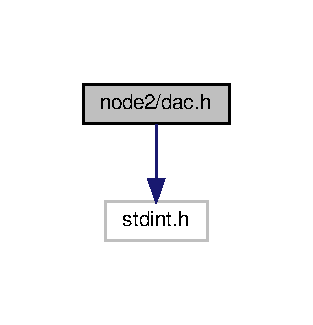
\includegraphics[width=150pt]{dac_8h__incl}
\end{center}
\end{figure}
This graph shows which files directly or indirectly include this file\+:\nopagebreak
\begin{figure}[H]
\begin{center}
\leavevmode
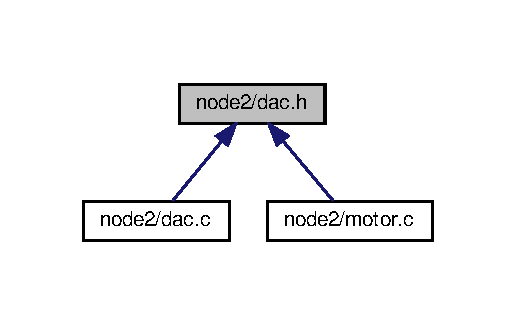
\includegraphics[width=248pt]{dac_8h__dep__incl}
\end{center}
\end{figure}
\subsection*{Functions}
\begin{DoxyCompactItemize}
\item 
\mbox{\Hypertarget{dac_8h_a6e622fafee8436bf9cf9f6b120352e3c}\label{dac_8h_a6e622fafee8436bf9cf9f6b120352e3c}} 
void \hyperlink{dac_8h_a6e622fafee8436bf9cf9f6b120352e3c}{dac\+\_\+init} (void)
\begin{DoxyCompactList}\small\item\em Initiates the D\+AC by setting its mode and clock source, choosing channel, and configuring its P\+MC settings. \end{DoxyCompactList}\item 
void \hyperlink{dac_8h_ab3ef2c4027995e3909bdb08a23251af5}{dac\+\_\+write} (uint16\+\_\+t data)
\begin{DoxyCompactList}\small\item\em Writes a value to be converted to an analog signal in the D\+AC. \end{DoxyCompactList}\end{DoxyCompactItemize}


\subsection{Detailed Description}
Module for dac-\/fuctionality. 



\subsection{Function Documentation}
\mbox{\Hypertarget{dac_8h_ab3ef2c4027995e3909bdb08a23251af5}\label{dac_8h_ab3ef2c4027995e3909bdb08a23251af5}} 
\index{dac.\+h@{dac.\+h}!dac\+\_\+write@{dac\+\_\+write}}
\index{dac\+\_\+write@{dac\+\_\+write}!dac.\+h@{dac.\+h}}
\subsubsection{\texorpdfstring{dac\+\_\+write()}{dac\_write()}}
{\footnotesize\ttfamily void dac\+\_\+write (\begin{DoxyParamCaption}\item[{uint16\+\_\+t}]{data }\end{DoxyParamCaption})}



Writes a value to be converted to an analog signal in the D\+AC. 


\begin{DoxyParams}{Parameters}
{\em data} & Data value to be converted to an analog signal. \\
\hline
\end{DoxyParams}


Definition at line 20 of file dac.\+c.


\hypertarget{game_8h}{}\section{node2/game.h File Reference}
\label{game_8h}\index{node2/game.\+h@{node2/game.\+h}}


Module for game-\/fuctionality.  


{\ttfamily \#include \char`\"{}../common/controller\+\_\+select.\+h\char`\"{}}\newline
{\ttfamily \#include \char`\"{}../common/difficulty\+\_\+select.\+h\char`\"{}}\newline
Include dependency graph for game.\+h\+:
\nopagebreak
\begin{figure}[H]
\begin{center}
\leavevmode
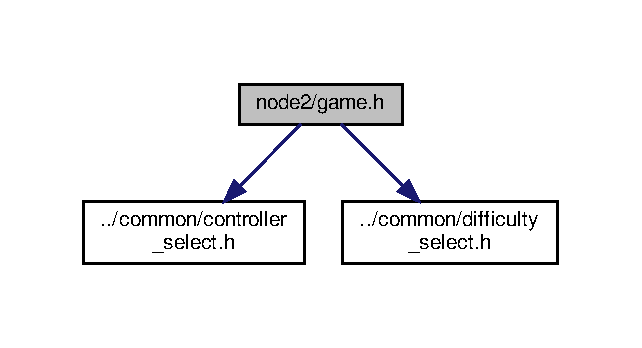
\includegraphics[width=308pt]{game_8h__incl}
\end{center}
\end{figure}
This graph shows which files directly or indirectly include this file\+:\nopagebreak
\begin{figure}[H]
\begin{center}
\leavevmode
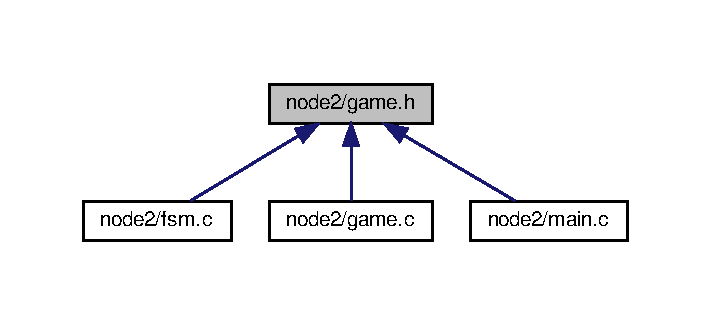
\includegraphics[width=341pt]{game_8h__dep__incl}
\end{center}
\end{figure}
\subsection*{Macros}
\begin{DoxyCompactItemize}
\item 
\mbox{\Hypertarget{game_8h_ac465bb46e4ee9f25d9f8ba918c1a21e9}\label{game_8h_ac465bb46e4ee9f25d9f8ba918c1a21e9}} 
\#define {\bfseries I\+N\+I\+T\+I\+A\+L\+\_\+\+L\+I\+V\+ES}~3
\end{DoxyCompactItemize}
\subsection*{Functions}
\begin{DoxyCompactItemize}
\item 
\mbox{\Hypertarget{game_8h_afe35a1f8874f44c04acfdec83ef9ef8e}\label{game_8h_afe35a1f8874f44c04acfdec83ef9ef8e}} 
void \hyperlink{game_8h_afe35a1f8874f44c04acfdec83ef9ef8e}{game\+\_\+init} (void)
\begin{DoxyCompactList}\small\item\em Initiates the game by resetting the score and lives left, enabling the timer for timed updating of the game signals, and initiating the P\+ID controller for the motor. \end{DoxyCompactList}\item 
int \hyperlink{game_8h_a797c47cfebac12385eb43746dfc167b4}{game\+\_\+count\+\_\+fails} (void)
\begin{DoxyCompactList}\small\item\em Checks if the IR beam is disrupted by the ball. Decreases the number of lives left if this is the case. \end{DoxyCompactList}\item 
void \hyperlink{game_8h_a7f8e8b2bc4d5263789aff1b40d71c55d}{game\+\_\+set\+\_\+user\+\_\+data} (char $\ast$data)
\begin{DoxyCompactList}\small\item\em Updates the user input data. \end{DoxyCompactList}\item 
void \hyperlink{game_8h_a4a32647b73e765a719fc4097bdc0fafe}{game\+\_\+set\+\_\+controller} (C\+O\+N\+T\+R\+O\+L\+L\+E\+R\+\_\+\+S\+EL controller)
\begin{DoxyCompactList}\small\item\em Selects the controller to be used in the game. \end{DoxyCompactList}\item 
void \hyperlink{game_8h_a02cb95b89dfad24606ed1e6ee0ece81e}{game\+\_\+set\+\_\+difficulty} (D\+I\+F\+F\+I\+C\+U\+L\+TY difficulty)
\begin{DoxyCompactList}\small\item\em Selects the difficulty to be used in the game. \end{DoxyCompactList}\item 
\mbox{\Hypertarget{game_8h_a3cc4819959534dcbb31b1c9f7f40615c}\label{game_8h_a3cc4819959534dcbb31b1c9f7f40615c}} 
void \hyperlink{game_8h_a3cc4819959534dcbb31b1c9f7f40615c}{game\+\_\+timer\+\_\+enable} ()
\begin{DoxyCompactList}\small\item\em Enables the timer which runs the game. \end{DoxyCompactList}\item 
\mbox{\Hypertarget{game_8h_a8cf447d101d6ef10f6dd0691566c2276}\label{game_8h_a8cf447d101d6ef10f6dd0691566c2276}} 
void \hyperlink{game_8h_a8cf447d101d6ef10f6dd0691566c2276}{game\+\_\+timer\+\_\+disable} ()
\begin{DoxyCompactList}\small\item\em Disables the timer which runs the game. \end{DoxyCompactList}\item 
int \hyperlink{game_8h_a05db567a17ee0823a4bed45e122d700c}{game\+\_\+get\+\_\+score} ()
\begin{DoxyCompactList}\small\item\em Returns the score of a game, which is increased by 50 every seconds. \end{DoxyCompactList}\item 
\mbox{\Hypertarget{game_8h_aab5c9885ccb80a787910546e0a304fcb}\label{game_8h_aab5c9885ccb80a787910546e0a304fcb}} 
void \hyperlink{game_8h_aab5c9885ccb80a787910546e0a304fcb}{game\+\_\+reset\+\_\+score} ()
\begin{DoxyCompactList}\small\item\em Resets the score of a game. \end{DoxyCompactList}\item 
\mbox{\Hypertarget{game_8h_a976b9ccf9cd4c3c354aee0f2bb6e1e4f}\label{game_8h_a976b9ccf9cd4c3c354aee0f2bb6e1e4f}} 
void \hyperlink{game_8h_a976b9ccf9cd4c3c354aee0f2bb6e1e4f}{game\+\_\+reset\+\_\+lives\+\_\+left} ()
\begin{DoxyCompactList}\small\item\em Resets the number of lives left in a game. \end{DoxyCompactList}\end{DoxyCompactItemize}


\subsection{Detailed Description}
Module for game-\/fuctionality. 



\subsection{Function Documentation}
\mbox{\Hypertarget{game_8h_a797c47cfebac12385eb43746dfc167b4}\label{game_8h_a797c47cfebac12385eb43746dfc167b4}} 
\index{game.\+h@{game.\+h}!game\+\_\+count\+\_\+fails@{game\+\_\+count\+\_\+fails}}
\index{game\+\_\+count\+\_\+fails@{game\+\_\+count\+\_\+fails}!game.\+h@{game.\+h}}
\subsubsection{\texorpdfstring{game\+\_\+count\+\_\+fails()}{game\_count\_fails()}}
{\footnotesize\ttfamily int game\+\_\+count\+\_\+fails (\begin{DoxyParamCaption}\item[{void}]{ }\end{DoxyParamCaption})}



Checks if the IR beam is disrupted by the ball. Decreases the number of lives left if this is the case. 

\begin{DoxyReturn}{Returns}
1 if the IR beam is disrupted, 0 if not. 
\end{DoxyReturn}


Definition at line 89 of file game.\+c.

\mbox{\Hypertarget{game_8h_a05db567a17ee0823a4bed45e122d700c}\label{game_8h_a05db567a17ee0823a4bed45e122d700c}} 
\index{game.\+h@{game.\+h}!game\+\_\+get\+\_\+score@{game\+\_\+get\+\_\+score}}
\index{game\+\_\+get\+\_\+score@{game\+\_\+get\+\_\+score}!game.\+h@{game.\+h}}
\subsubsection{\texorpdfstring{game\+\_\+get\+\_\+score()}{game\_get\_score()}}
{\footnotesize\ttfamily int game\+\_\+get\+\_\+score (\begin{DoxyParamCaption}{ }\end{DoxyParamCaption})}



Returns the score of a game, which is increased by 50 every seconds. 

\begin{DoxyReturn}{Returns}
The score of a game. 
\end{DoxyReturn}


Definition at line 201 of file game.\+c.

\mbox{\Hypertarget{game_8h_a4a32647b73e765a719fc4097bdc0fafe}\label{game_8h_a4a32647b73e765a719fc4097bdc0fafe}} 
\index{game.\+h@{game.\+h}!game\+\_\+set\+\_\+controller@{game\+\_\+set\+\_\+controller}}
\index{game\+\_\+set\+\_\+controller@{game\+\_\+set\+\_\+controller}!game.\+h@{game.\+h}}
\subsubsection{\texorpdfstring{game\+\_\+set\+\_\+controller()}{game\_set\_controller()}}
{\footnotesize\ttfamily void game\+\_\+set\+\_\+controller (\begin{DoxyParamCaption}\item[{C\+O\+N\+T\+R\+O\+L\+L\+E\+R\+\_\+\+S\+EL}]{controller }\end{DoxyParamCaption})}



Selects the controller to be used in the game. 


\begin{DoxyParams}{Parameters}
{\em controller} & The controller option of data type {\ttfamily C\+O\+N\+T\+R\+O\+L\+L\+E\+R\+\_\+\+S\+EL} to be used in the game. \\
\hline
\end{DoxyParams}


Definition at line 107 of file game.\+c.

\mbox{\Hypertarget{game_8h_a02cb95b89dfad24606ed1e6ee0ece81e}\label{game_8h_a02cb95b89dfad24606ed1e6ee0ece81e}} 
\index{game.\+h@{game.\+h}!game\+\_\+set\+\_\+difficulty@{game\+\_\+set\+\_\+difficulty}}
\index{game\+\_\+set\+\_\+difficulty@{game\+\_\+set\+\_\+difficulty}!game.\+h@{game.\+h}}
\subsubsection{\texorpdfstring{game\+\_\+set\+\_\+difficulty()}{game\_set\_difficulty()}}
{\footnotesize\ttfamily void game\+\_\+set\+\_\+difficulty (\begin{DoxyParamCaption}\item[{D\+I\+F\+F\+I\+C\+U\+L\+TY}]{difficulty }\end{DoxyParamCaption})}



Selects the difficulty to be used in the game. 


\begin{DoxyParams}{Parameters}
{\em controller} & The difficulty option of data type {\ttfamily D\+I\+F\+F\+I\+C\+U\+L\+TY} to be used in the game. \\
\hline
\end{DoxyParams}


Definition at line 112 of file game.\+c.

\mbox{\Hypertarget{game_8h_a7f8e8b2bc4d5263789aff1b40d71c55d}\label{game_8h_a7f8e8b2bc4d5263789aff1b40d71c55d}} 
\index{game.\+h@{game.\+h}!game\+\_\+set\+\_\+user\+\_\+data@{game\+\_\+set\+\_\+user\+\_\+data}}
\index{game\+\_\+set\+\_\+user\+\_\+data@{game\+\_\+set\+\_\+user\+\_\+data}!game.\+h@{game.\+h}}
\subsubsection{\texorpdfstring{game\+\_\+set\+\_\+user\+\_\+data()}{game\_set\_user\_data()}}
{\footnotesize\ttfamily void game\+\_\+set\+\_\+user\+\_\+data (\begin{DoxyParamCaption}\item[{char $\ast$}]{data }\end{DoxyParamCaption})}



Updates the user input data. 


\begin{DoxyParams}{Parameters}
{\em data} & An array with new user input data, in the order \{joystick.\+x, joystick.\+y, slider.\+right, slider.\+left, buttons.\+left, buttons.\+right\}. \\
\hline
\end{DoxyParams}


Definition at line 138 of file game.\+c.


\hypertarget{led_8h}{}\section{node2/led.h File Reference}
\label{led_8h}\index{node2/led.\+h@{node2/led.\+h}}


Module for led-\/fuctionality.  


This graph shows which files directly or indirectly include this file\+:\nopagebreak
\begin{figure}[H]
\begin{center}
\leavevmode
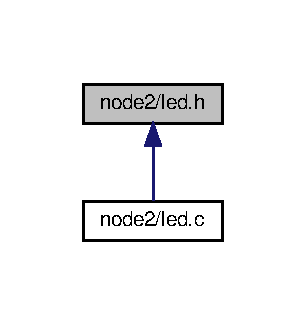
\includegraphics[width=147pt]{led_8h__dep__incl}
\end{center}
\end{figure}
\subsection*{Functions}
\begin{DoxyCompactItemize}
\item 
\mbox{\Hypertarget{led_8h_a053c30480e135459f0bb97621e289053}\label{led_8h_a053c30480e135459f0bb97621e289053}} 
void \hyperlink{led_8h_a053c30480e135459f0bb97621e289053}{led\+\_\+set} (void)
\begin{DoxyCompactList}\small\item\em Set the led-\/lights on the arduino. \end{DoxyCompactList}\end{DoxyCompactItemize}


\subsection{Detailed Description}
Module for led-\/fuctionality. 


\hypertarget{microbit_8h}{}\section{node2/microbit.h File Reference}
\label{microbit_8h}\index{node2/microbit.\+h@{node2/microbit.\+h}}


Module for microbit functionality.  


{\ttfamily \#include \char`\"{}../node3/source/controller.\+h\char`\"{}}\newline
Include dependency graph for microbit.\+h\+:\nopagebreak
\begin{figure}[H]
\begin{center}
\leavevmode
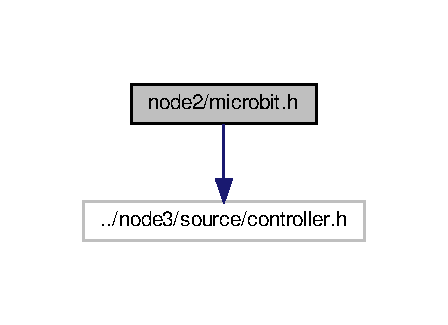
\includegraphics[width=215pt]{microbit_8h__incl}
\end{center}
\end{figure}
This graph shows which files directly or indirectly include this file\+:\nopagebreak
\begin{figure}[H]
\begin{center}
\leavevmode
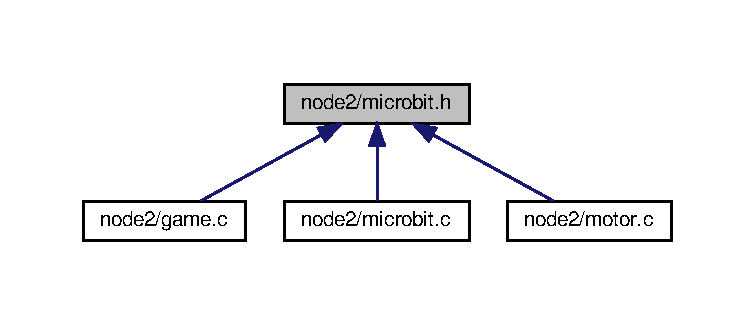
\includegraphics[width=350pt]{microbit_8h__dep__incl}
\end{center}
\end{figure}
\subsection*{Functions}
\begin{DoxyCompactItemize}
\item 
\mbox{\Hypertarget{microbit_8h_a09e9f665d32bbfc6b7c0e0c5357b89ed}\label{microbit_8h_a09e9f665d32bbfc6b7c0e0c5357b89ed}} 
void \hyperlink{microbit_8h_a09e9f665d32bbfc6b7c0e0c5357b89ed}{microbit\+\_\+init} ()
\begin{DoxyCompactList}\small\item\em Initializes the microbit by enabling the P\+IO to control the corresponding pins. \end{DoxyCompactList}\item 
const acc\+\_\+dir\+\_\+t \hyperlink{microbit_8h_aba863f04abafc073cc63668e99e783f9}{microbit\+\_\+dir} ()
\begin{DoxyCompactList}\small\item\em Returns the microbit accelerometer output. \end{DoxyCompactList}\item 
const char \hyperlink{microbit_8h_a07adcd1fa85aa0fabc77968ec697ec70}{microbit\+\_\+button} ()
\begin{DoxyCompactList}\small\item\em Returns the microbit left button output. \end{DoxyCompactList}\end{DoxyCompactItemize}


\subsection{Detailed Description}
Module for microbit functionality. 



\subsection{Function Documentation}
\mbox{\Hypertarget{microbit_8h_a07adcd1fa85aa0fabc77968ec697ec70}\label{microbit_8h_a07adcd1fa85aa0fabc77968ec697ec70}} 
\index{microbit.\+h@{microbit.\+h}!microbit\+\_\+button@{microbit\+\_\+button}}
\index{microbit\+\_\+button@{microbit\+\_\+button}!microbit.\+h@{microbit.\+h}}
\subsubsection{\texorpdfstring{microbit\+\_\+button()}{microbit\_button()}}
{\footnotesize\ttfamily const char microbit\+\_\+button (\begin{DoxyParamCaption}{ }\end{DoxyParamCaption})}



Returns the microbit left button output. 

\begin{DoxyReturn}{Returns}
Returns 1 if pressed, 0 otherwise 
\end{DoxyReturn}


Definition at line 31 of file microbit.\+c.

\mbox{\Hypertarget{microbit_8h_aba863f04abafc073cc63668e99e783f9}\label{microbit_8h_aba863f04abafc073cc63668e99e783f9}} 
\index{microbit.\+h@{microbit.\+h}!microbit\+\_\+dir@{microbit\+\_\+dir}}
\index{microbit\+\_\+dir@{microbit\+\_\+dir}!microbit.\+h@{microbit.\+h}}
\subsubsection{\texorpdfstring{microbit\+\_\+dir()}{microbit\_dir()}}
{\footnotesize\ttfamily const acc\+\_\+dir\+\_\+t microbit\+\_\+dir (\begin{DoxyParamCaption}{ }\end{DoxyParamCaption})}



Returns the microbit accelerometer output. 

\begin{DoxyReturn}{Returns}
Returns either A\+C\+C\+\_\+\+L\+E\+FT, A\+C\+C\+\_\+\+M\+I\+D\+D\+LE, A\+C\+C\+\_\+\+R\+I\+G\+HT 
\end{DoxyReturn}


Definition at line 19 of file microbit.\+c.


\hypertarget{motor_8h}{}\section{node2/motor.h File Reference}
\label{motor_8h}\index{node2/motor.\+h@{node2/motor.\+h}}


Module for motor functionality.  


{\ttfamily \#include $<$stdint.\+h$>$}\newline
Include dependency graph for motor.\+h\+:\nopagebreak
\begin{figure}[H]
\begin{center}
\leavevmode
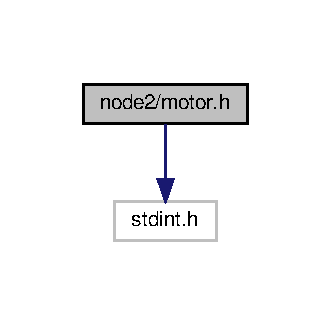
\includegraphics[width=159pt]{motor_8h__incl}
\end{center}
\end{figure}
This graph shows which files directly or indirectly include this file\+:\nopagebreak
\begin{figure}[H]
\begin{center}
\leavevmode
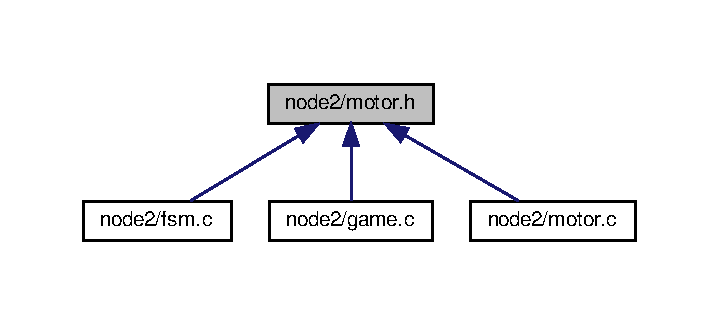
\includegraphics[width=345pt]{motor_8h__dep__incl}
\end{center}
\end{figure}
\subsection*{Macros}
\begin{DoxyCompactItemize}
\item 
\mbox{\Hypertarget{motor_8h_a6c8de73bb604d91743c7f6f356eb171e}\label{motor_8h_a6c8de73bb604d91743c7f6f356eb171e}} 
\#define {\bfseries D\+IR}~P\+I\+O\+\_\+\+P\+D10
\item 
\mbox{\Hypertarget{motor_8h_a22e6626f2c98ed902f8ded47f6438c05}\label{motor_8h_a22e6626f2c98ed902f8ded47f6438c05}} 
\#define {\bfseries EN}~P\+I\+O\+\_\+\+P\+D9
\item 
\mbox{\Hypertarget{motor_8h_a66c7f87d14d4591f214e44dc70c05454}\label{motor_8h_a66c7f87d14d4591f214e44dc70c05454}} 
\#define {\bfseries S\+EL}~P\+I\+O\+\_\+\+P\+D2
\item 
\mbox{\Hypertarget{motor_8h_a3df39239a243fc43430ef2f6fc42af0a}\label{motor_8h_a3df39239a243fc43430ef2f6fc42af0a}} 
\#define {\bfseries N\+O\+T\+\_\+\+R\+ST}~P\+I\+O\+\_\+\+P\+D1
\item 
\mbox{\Hypertarget{motor_8h_aa01edc4557d0fe59ab1df0342fdfedfe}\label{motor_8h_aa01edc4557d0fe59ab1df0342fdfedfe}} 
\#define {\bfseries N\+O\+T\+\_\+\+OE}~P\+I\+O\+\_\+\+P\+D0
\item 
\mbox{\Hypertarget{motor_8h_a2a66705260c7a3f99a155382c167cec5}\label{motor_8h_a2a66705260c7a3f99a155382c167cec5}} 
\#define {\bfseries D\+O0\+\_\+\+I\+DX}~1
\item 
\mbox{\Hypertarget{motor_8h_a0b4d5a65a3c1fedf540eb0fcb0b9c855}\label{motor_8h_a0b4d5a65a3c1fedf540eb0fcb0b9c855}} 
\#define {\bfseries M\+O\+T\+O\+R\+\_\+\+T\+I\+M\+E\+R\+\_\+\+F\+R\+EQ}~50
\end{DoxyCompactItemize}
\subsection*{Functions}
\begin{DoxyCompactItemize}
\item 
\mbox{\Hypertarget{motor_8h_aa2a5af0fb9c1fa2047a5ca0af110f806}\label{motor_8h_aa2a5af0fb9c1fa2047a5ca0af110f806}} 
void \hyperlink{motor_8h_aa2a5af0fb9c1fa2047a5ca0af110f806}{motor\+\_\+init} (void)
\begin{DoxyCompactList}\small\item\em Initiates the motor by initiating the D\+AC, and enabling the pins and clock used by the motor. \end{DoxyCompactList}\item 
\mbox{\Hypertarget{motor_8h_a024679ab792710e4c0f1800b8cda0834}\label{motor_8h_a024679ab792710e4c0f1800b8cda0834}} 
void \hyperlink{motor_8h_a024679ab792710e4c0f1800b8cda0834}{motor\+\_\+disable} (void)
\begin{DoxyCompactList}\small\item\em Disables the motor. Sets the speed to 0. \end{DoxyCompactList}\item 
\mbox{\Hypertarget{motor_8h_a8d3f3c8b0807d3879f832e346e86c0c2}\label{motor_8h_a8d3f3c8b0807d3879f832e346e86c0c2}} 
void \hyperlink{motor_8h_a8d3f3c8b0807d3879f832e346e86c0c2}{motor\+\_\+enable} (void)
\begin{DoxyCompactList}\small\item\em Enables the motor. Resets the P\+ID errors. \end{DoxyCompactList}\item 
int \hyperlink{motor_8h_a45b940e7cd61a2fedd2b666082832ad7}{motor\+\_\+read\+\_\+encoder} (void)
\begin{DoxyCompactList}\small\item\em Reads the motor encoder. \end{DoxyCompactList}\item 
void \hyperlink{motor_8h_ac41cb93592f494a7078568b425260cc3}{motor\+\_\+run\+\_\+slider} (int reference)
\begin{DoxyCompactList}\small\item\em Uses the P\+ID controller to drive the motor, by comparing the encoder measurement to the input {\ttfamily reference}. \end{DoxyCompactList}\item 
void \hyperlink{motor_8h_a7922f5fd00c58af20b34e39bdcd397bf}{motor\+\_\+run\+\_\+joystick} (int joystick\+\_\+value)
\begin{DoxyCompactList}\small\item\em Drives the motor speed, by comparing the encoder measurement to the input {\ttfamily reference}. \end{DoxyCompactList}\item 
\mbox{\Hypertarget{motor_8h_a5f704ee67b11a2ec95459393e6fae7bf}\label{motor_8h_a5f704ee67b11a2ec95459393e6fae7bf}} 
void \hyperlink{motor_8h_a5f704ee67b11a2ec95459393e6fae7bf}{motor\+\_\+run\+\_\+microbit} ()
\begin{DoxyCompactList}\small\item\em Drives the motor by reading the accelerometer output from the microbit. \end{DoxyCompactList}\end{DoxyCompactItemize}


\subsection{Detailed Description}
Module for motor functionality. 



\subsection{Function Documentation}
\mbox{\Hypertarget{motor_8h_a45b940e7cd61a2fedd2b666082832ad7}\label{motor_8h_a45b940e7cd61a2fedd2b666082832ad7}} 
\index{motor.\+h@{motor.\+h}!motor\+\_\+read\+\_\+encoder@{motor\+\_\+read\+\_\+encoder}}
\index{motor\+\_\+read\+\_\+encoder@{motor\+\_\+read\+\_\+encoder}!motor.\+h@{motor.\+h}}
\subsubsection{\texorpdfstring{motor\+\_\+read\+\_\+encoder()}{motor\_read\_encoder()}}
{\footnotesize\ttfamily int motor\+\_\+read\+\_\+encoder (\begin{DoxyParamCaption}\item[{void}]{ }\end{DoxyParamCaption})}



Reads the motor encoder. 

\begin{DoxyReturn}{Returns}
The read encoder value. 
\end{DoxyReturn}


Definition at line 78 of file motor.\+c.

\mbox{\Hypertarget{motor_8h_a7922f5fd00c58af20b34e39bdcd397bf}\label{motor_8h_a7922f5fd00c58af20b34e39bdcd397bf}} 
\index{motor.\+h@{motor.\+h}!motor\+\_\+run\+\_\+joystick@{motor\+\_\+run\+\_\+joystick}}
\index{motor\+\_\+run\+\_\+joystick@{motor\+\_\+run\+\_\+joystick}!motor.\+h@{motor.\+h}}
\subsubsection{\texorpdfstring{motor\+\_\+run\+\_\+joystick()}{motor\_run\_joystick()}}
{\footnotesize\ttfamily void motor\+\_\+run\+\_\+joystick (\begin{DoxyParamCaption}\item[{int}]{joystick\+\_\+value }\end{DoxyParamCaption})}



Drives the motor speed, by comparing the encoder measurement to the input {\ttfamily reference}. 


\begin{DoxyParams}{Parameters}
{\em joystick\+\_\+value} & The reference value joystick position. \\
\hline
\end{DoxyParams}


Definition at line 126 of file motor.\+c.

\mbox{\Hypertarget{motor_8h_ac41cb93592f494a7078568b425260cc3}\label{motor_8h_ac41cb93592f494a7078568b425260cc3}} 
\index{motor.\+h@{motor.\+h}!motor\+\_\+run\+\_\+slider@{motor\+\_\+run\+\_\+slider}}
\index{motor\+\_\+run\+\_\+slider@{motor\+\_\+run\+\_\+slider}!motor.\+h@{motor.\+h}}
\subsubsection{\texorpdfstring{motor\+\_\+run\+\_\+slider()}{motor\_run\_slider()}}
{\footnotesize\ttfamily void motor\+\_\+run\+\_\+slider (\begin{DoxyParamCaption}\item[{int}]{reference }\end{DoxyParamCaption})}



Uses the P\+ID controller to drive the motor, by comparing the encoder measurement to the input {\ttfamily reference}. 


\begin{DoxyParams}{Parameters}
{\em reference} & The reference value input to the P\+ID controller. \\
\hline
\end{DoxyParams}


Definition at line 108 of file motor.\+c.


\hypertarget{music__driver_8h}{}\section{node2/music\+\_\+driver.h File Reference}
\label{music__driver_8h}\index{node2/music\+\_\+driver.\+h@{node2/music\+\_\+driver.\+h}}


Module for music functionality.  


{\ttfamily \#include \char`\"{}../common/songs.\+h\char`\"{}}\newline
Include dependency graph for music\+\_\+driver.\+h\+:
\nopagebreak
\begin{figure}[H]
\begin{center}
\leavevmode
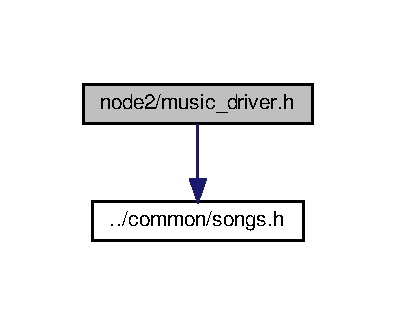
\includegraphics[width=190pt]{music__driver_8h__incl}
\end{center}
\end{figure}
This graph shows which files directly or indirectly include this file\+:\nopagebreak
\begin{figure}[H]
\begin{center}
\leavevmode
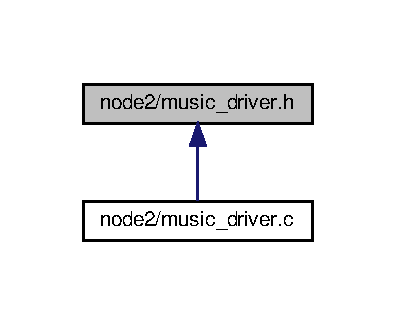
\includegraphics[width=190pt]{music__driver_8h__dep__incl}
\end{center}
\end{figure}
\subsection*{Functions}
\begin{DoxyCompactItemize}
\item 
\mbox{\Hypertarget{music__driver_8h_a146ada1dade5ae8e55dd20280c251188}\label{music__driver_8h_a146ada1dade5ae8e55dd20280c251188}} 
void \hyperlink{music__driver_8h_a146ada1dade5ae8e55dd20280c251188}{music\+\_\+play} (S\+O\+NG song)
\begin{DoxyCompactList}\small\item\em Plays a song {\ttfamily song} through a P\+WM signal fed to a buzzer. \end{DoxyCompactList}\end{DoxyCompactItemize}


\subsection{Detailed Description}
Module for music functionality. 


\hypertarget{music__metadata_8h}{}\section{node2/music\+\_\+metadata.h File Reference}
\label{music__metadata_8h}\index{node2/music\+\_\+metadata.\+h@{node2/music\+\_\+metadata.\+h}}


Module for song notes.  


This graph shows which files directly or indirectly include this file\+:\nopagebreak
\begin{figure}[H]
\begin{center}
\leavevmode
\includegraphics[width=206pt]{music__metadata_8h__dep__incl}
\end{center}
\end{figure}
\subsection*{Macros}
\begin{DoxyCompactItemize}
\item 
\mbox{\Hypertarget{music__metadata_8h_a75daabb2226536982e7cd233cd1e6f39}\label{music__metadata_8h_a75daabb2226536982e7cd233cd1e6f39}} 
\#define \hyperlink{music__metadata_8h_a75daabb2226536982e7cd233cd1e6f39}{N\+O\+T\+E\+\_\+\+B0}~31
\begin{DoxyCompactList}\small\item\em Frequencies of corresponding notes. \end{DoxyCompactList}\item 
\mbox{\Hypertarget{music__metadata_8h_a3967a2d455ebdbe5e51db21bfb17fe85}\label{music__metadata_8h_a3967a2d455ebdbe5e51db21bfb17fe85}} 
\#define {\bfseries N\+O\+T\+E\+\_\+\+C1}~33
\item 
\mbox{\Hypertarget{music__metadata_8h_a860b429370d8c2d7a1c4dbd66b4bcfaa}\label{music__metadata_8h_a860b429370d8c2d7a1c4dbd66b4bcfaa}} 
\#define {\bfseries N\+O\+T\+E\+\_\+\+C\+S1}~35
\item 
\mbox{\Hypertarget{music__metadata_8h_a6fccac36e451f74157b234d64260b92e}\label{music__metadata_8h_a6fccac36e451f74157b234d64260b92e}} 
\#define {\bfseries N\+O\+T\+E\+\_\+\+D1}~37
\item 
\mbox{\Hypertarget{music__metadata_8h_ac9a118b2bfc4c7208afc2db45c80b5a0}\label{music__metadata_8h_ac9a118b2bfc4c7208afc2db45c80b5a0}} 
\#define {\bfseries N\+O\+T\+E\+\_\+\+D\+S1}~39
\item 
\mbox{\Hypertarget{music__metadata_8h_a0132d10523bb1a91b0aac0a47aee4dbe}\label{music__metadata_8h_a0132d10523bb1a91b0aac0a47aee4dbe}} 
\#define {\bfseries N\+O\+T\+E\+\_\+\+E1}~41
\item 
\mbox{\Hypertarget{music__metadata_8h_a8b7abe19db306650a9c0e5e2c7fd98e2}\label{music__metadata_8h_a8b7abe19db306650a9c0e5e2c7fd98e2}} 
\#define {\bfseries N\+O\+T\+E\+\_\+\+F1}~44
\item 
\mbox{\Hypertarget{music__metadata_8h_a9ab5c314120ca69e5547b6848b5f2220}\label{music__metadata_8h_a9ab5c314120ca69e5547b6848b5f2220}} 
\#define {\bfseries N\+O\+T\+E\+\_\+\+F\+S1}~46
\item 
\mbox{\Hypertarget{music__metadata_8h_a45789d849fd75408a30c5cfb35e164d9}\label{music__metadata_8h_a45789d849fd75408a30c5cfb35e164d9}} 
\#define {\bfseries N\+O\+T\+E\+\_\+\+G1}~49
\item 
\mbox{\Hypertarget{music__metadata_8h_a6cb0879026575ff13753e45023f98c54}\label{music__metadata_8h_a6cb0879026575ff13753e45023f98c54}} 
\#define {\bfseries N\+O\+T\+E\+\_\+\+G\+S1}~52
\item 
\mbox{\Hypertarget{music__metadata_8h_ae7263a79e9675b3bae2b73d2c8b7d0f8}\label{music__metadata_8h_ae7263a79e9675b3bae2b73d2c8b7d0f8}} 
\#define {\bfseries N\+O\+T\+E\+\_\+\+A1}~55
\item 
\mbox{\Hypertarget{music__metadata_8h_acfcb8b2ac851e6f7b76610b28d21cf85}\label{music__metadata_8h_acfcb8b2ac851e6f7b76610b28d21cf85}} 
\#define {\bfseries N\+O\+T\+E\+\_\+\+A\+S1}~58
\item 
\mbox{\Hypertarget{music__metadata_8h_a05b80b905f142f5ffc29b52f4e92fda1}\label{music__metadata_8h_a05b80b905f142f5ffc29b52f4e92fda1}} 
\#define {\bfseries N\+O\+T\+E\+\_\+\+B1}~62
\item 
\mbox{\Hypertarget{music__metadata_8h_a83e1f6d716a3f6560aa1d43b8245855d}\label{music__metadata_8h_a83e1f6d716a3f6560aa1d43b8245855d}} 
\#define {\bfseries N\+O\+T\+E\+\_\+\+C2}~65
\item 
\mbox{\Hypertarget{music__metadata_8h_a0e1ed6d231ab36b54a5a894e76836872}\label{music__metadata_8h_a0e1ed6d231ab36b54a5a894e76836872}} 
\#define {\bfseries N\+O\+T\+E\+\_\+\+C\+S2}~69
\item 
\mbox{\Hypertarget{music__metadata_8h_ad219c7bf8aee3d671c24c760d1eac336}\label{music__metadata_8h_ad219c7bf8aee3d671c24c760d1eac336}} 
\#define {\bfseries N\+O\+T\+E\+\_\+\+D2}~73
\item 
\mbox{\Hypertarget{music__metadata_8h_a189cef9016942455b464b47faec10f7c}\label{music__metadata_8h_a189cef9016942455b464b47faec10f7c}} 
\#define {\bfseries N\+O\+T\+E\+\_\+\+D\+S2}~78
\item 
\mbox{\Hypertarget{music__metadata_8h_a9a021ea5eaee62fd52d4f67250712abb}\label{music__metadata_8h_a9a021ea5eaee62fd52d4f67250712abb}} 
\#define {\bfseries N\+O\+T\+E\+\_\+\+E2}~82
\item 
\mbox{\Hypertarget{music__metadata_8h_a55ebff842099b32c7e80f0870df9730e}\label{music__metadata_8h_a55ebff842099b32c7e80f0870df9730e}} 
\#define {\bfseries N\+O\+T\+E\+\_\+\+F2}~87
\item 
\mbox{\Hypertarget{music__metadata_8h_a3926c1af05e2876f1e9870566c09049e}\label{music__metadata_8h_a3926c1af05e2876f1e9870566c09049e}} 
\#define {\bfseries N\+O\+T\+E\+\_\+\+F\+S2}~93
\item 
\mbox{\Hypertarget{music__metadata_8h_a0a94df54731934347951149740d9eac0}\label{music__metadata_8h_a0a94df54731934347951149740d9eac0}} 
\#define {\bfseries N\+O\+T\+E\+\_\+\+G2}~98
\item 
\mbox{\Hypertarget{music__metadata_8h_a70347f8b8ad83fde025d45d0692286f6}\label{music__metadata_8h_a70347f8b8ad83fde025d45d0692286f6}} 
\#define {\bfseries N\+O\+T\+E\+\_\+\+G\+S2}~104
\item 
\mbox{\Hypertarget{music__metadata_8h_ad8c52bd098530d4253e7433c8cc29ee9}\label{music__metadata_8h_ad8c52bd098530d4253e7433c8cc29ee9}} 
\#define {\bfseries N\+O\+T\+E\+\_\+\+A2}~110
\item 
\mbox{\Hypertarget{music__metadata_8h_af0d7a5be59334bf1985cbddde34b95bb}\label{music__metadata_8h_af0d7a5be59334bf1985cbddde34b95bb}} 
\#define {\bfseries N\+O\+T\+E\+\_\+\+A\+S2}~117
\item 
\mbox{\Hypertarget{music__metadata_8h_a49bbf78568a8e133862a1c84b825b678}\label{music__metadata_8h_a49bbf78568a8e133862a1c84b825b678}} 
\#define {\bfseries N\+O\+T\+E\+\_\+\+B2}~123
\item 
\mbox{\Hypertarget{music__metadata_8h_aa0630dbc2c704089b77bda35dfea855b}\label{music__metadata_8h_aa0630dbc2c704089b77bda35dfea855b}} 
\#define {\bfseries N\+O\+T\+E\+\_\+\+C3}~131
\item 
\mbox{\Hypertarget{music__metadata_8h_a8086c9cb19cdacd01d2f0ffde5885f8b}\label{music__metadata_8h_a8086c9cb19cdacd01d2f0ffde5885f8b}} 
\#define {\bfseries N\+O\+T\+E\+\_\+\+C\+S3}~139
\item 
\mbox{\Hypertarget{music__metadata_8h_a9e892b1e2743a11f7a4ce61f1b15688f}\label{music__metadata_8h_a9e892b1e2743a11f7a4ce61f1b15688f}} 
\#define {\bfseries N\+O\+T\+E\+\_\+\+D3}~147
\item 
\mbox{\Hypertarget{music__metadata_8h_a233fdbde84ffdd12523bf1c0bef152eb}\label{music__metadata_8h_a233fdbde84ffdd12523bf1c0bef152eb}} 
\#define {\bfseries N\+O\+T\+E\+\_\+\+D\+S3}~156
\item 
\mbox{\Hypertarget{music__metadata_8h_a31913cf742bcbe91a39a47e819ac289c}\label{music__metadata_8h_a31913cf742bcbe91a39a47e819ac289c}} 
\#define {\bfseries N\+O\+T\+E\+\_\+\+E3}~165
\item 
\mbox{\Hypertarget{music__metadata_8h_a2533a6044529da9ea46ea98e76ee50ad}\label{music__metadata_8h_a2533a6044529da9ea46ea98e76ee50ad}} 
\#define {\bfseries N\+O\+T\+E\+\_\+\+F3}~175
\item 
\mbox{\Hypertarget{music__metadata_8h_a2c1622ffe3f5cd463de2964742571e02}\label{music__metadata_8h_a2c1622ffe3f5cd463de2964742571e02}} 
\#define {\bfseries N\+O\+T\+E\+\_\+\+F\+S3}~185
\item 
\mbox{\Hypertarget{music__metadata_8h_a60b70b4fe537257e776eafd46d25e49b}\label{music__metadata_8h_a60b70b4fe537257e776eafd46d25e49b}} 
\#define {\bfseries N\+O\+T\+E\+\_\+\+G3}~196
\item 
\mbox{\Hypertarget{music__metadata_8h_ae2b3de8c17ba8ae7e2e758c6b15576ca}\label{music__metadata_8h_ae2b3de8c17ba8ae7e2e758c6b15576ca}} 
\#define {\bfseries N\+O\+T\+E\+\_\+\+G\+S3}~208
\item 
\mbox{\Hypertarget{music__metadata_8h_a934b0ccc182054ca8da5c67c0e78a04c}\label{music__metadata_8h_a934b0ccc182054ca8da5c67c0e78a04c}} 
\#define {\bfseries N\+O\+T\+E\+\_\+\+A3}~220
\item 
\mbox{\Hypertarget{music__metadata_8h_a33992ffb6f31579b376cef8c5858b9f0}\label{music__metadata_8h_a33992ffb6f31579b376cef8c5858b9f0}} 
\#define {\bfseries N\+O\+T\+E\+\_\+\+A\+S3}~233
\item 
\mbox{\Hypertarget{music__metadata_8h_aa5207dfb3103215cdb89a40c1753eea8}\label{music__metadata_8h_aa5207dfb3103215cdb89a40c1753eea8}} 
\#define {\bfseries N\+O\+T\+E\+\_\+\+B3}~247
\item 
\mbox{\Hypertarget{music__metadata_8h_adbed706152a3d7114327fc5af3c7e07c}\label{music__metadata_8h_adbed706152a3d7114327fc5af3c7e07c}} 
\#define {\bfseries N\+O\+T\+E\+\_\+\+C4}~262
\item 
\mbox{\Hypertarget{music__metadata_8h_ae9a1fa0e819ea29161a72b6840dd0ffc}\label{music__metadata_8h_ae9a1fa0e819ea29161a72b6840dd0ffc}} 
\#define {\bfseries N\+O\+T\+E\+\_\+\+C\+S4}~277
\item 
\mbox{\Hypertarget{music__metadata_8h_a6162f78ec6fc3457a077602a77e36992}\label{music__metadata_8h_a6162f78ec6fc3457a077602a77e36992}} 
\#define {\bfseries N\+O\+T\+E\+\_\+\+D4}~294
\item 
\mbox{\Hypertarget{music__metadata_8h_a638f884f0226cff11eff97ba96fbce88}\label{music__metadata_8h_a638f884f0226cff11eff97ba96fbce88}} 
\#define {\bfseries N\+O\+T\+E\+\_\+\+D\+S4}~311
\item 
\mbox{\Hypertarget{music__metadata_8h_a147e4663d8161df841c418859a70f66f}\label{music__metadata_8h_a147e4663d8161df841c418859a70f66f}} 
\#define {\bfseries N\+O\+T\+E\+\_\+\+E4}~330
\item 
\mbox{\Hypertarget{music__metadata_8h_aff20d9abb2ef6f25afeb44245129eba6}\label{music__metadata_8h_aff20d9abb2ef6f25afeb44245129eba6}} 
\#define {\bfseries N\+O\+T\+E\+\_\+\+F4}~349
\item 
\mbox{\Hypertarget{music__metadata_8h_a3ca197d6b74ace12c6cc9e53f47b7a6a}\label{music__metadata_8h_a3ca197d6b74ace12c6cc9e53f47b7a6a}} 
\#define {\bfseries N\+O\+T\+E\+\_\+\+F\+S4}~370
\item 
\mbox{\Hypertarget{music__metadata_8h_a588324691d836c7cdf1dd8cc071eeecc}\label{music__metadata_8h_a588324691d836c7cdf1dd8cc071eeecc}} 
\#define {\bfseries N\+O\+T\+E\+\_\+\+G4}~392
\item 
\mbox{\Hypertarget{music__metadata_8h_ac446a7c56b75b56451b6712833bfd31f}\label{music__metadata_8h_ac446a7c56b75b56451b6712833bfd31f}} 
\#define {\bfseries N\+O\+T\+E\+\_\+\+G\+S4}~415
\item 
\mbox{\Hypertarget{music__metadata_8h_a4ede898d3fa744ffb02d5e9b66994ef3}\label{music__metadata_8h_a4ede898d3fa744ffb02d5e9b66994ef3}} 
\#define {\bfseries N\+O\+T\+E\+\_\+\+A4}~440
\item 
\mbox{\Hypertarget{music__metadata_8h_aaf4ee3ef21f5803c75089341e7e3f50d}\label{music__metadata_8h_aaf4ee3ef21f5803c75089341e7e3f50d}} 
\#define {\bfseries N\+O\+T\+E\+\_\+\+A\+S4}~466
\item 
\mbox{\Hypertarget{music__metadata_8h_a9ed6d5c8563ae60e6d2716e13d261386}\label{music__metadata_8h_a9ed6d5c8563ae60e6d2716e13d261386}} 
\#define {\bfseries N\+O\+T\+E\+\_\+\+B4}~494
\item 
\mbox{\Hypertarget{music__metadata_8h_a8afb484cf5507628f20dd2822a5b2e79}\label{music__metadata_8h_a8afb484cf5507628f20dd2822a5b2e79}} 
\#define {\bfseries N\+O\+T\+E\+\_\+\+C5}~523
\item 
\mbox{\Hypertarget{music__metadata_8h_a8f01a2997f769170cc4f20287aca5339}\label{music__metadata_8h_a8f01a2997f769170cc4f20287aca5339}} 
\#define {\bfseries N\+O\+T\+E\+\_\+\+C\+S5}~554
\item 
\mbox{\Hypertarget{music__metadata_8h_a37abdd5b16959e6265e7de75022f5dde}\label{music__metadata_8h_a37abdd5b16959e6265e7de75022f5dde}} 
\#define {\bfseries N\+O\+T\+E\+\_\+\+D5}~587
\item 
\mbox{\Hypertarget{music__metadata_8h_a7943ad2d66e53367906e04e8af1c086a}\label{music__metadata_8h_a7943ad2d66e53367906e04e8af1c086a}} 
\#define {\bfseries N\+O\+T\+E\+\_\+\+D\+S5}~622
\item 
\mbox{\Hypertarget{music__metadata_8h_a441475178599565b3dd4572cebbdf28c}\label{music__metadata_8h_a441475178599565b3dd4572cebbdf28c}} 
\#define {\bfseries N\+O\+T\+E\+\_\+\+E5}~659
\item 
\mbox{\Hypertarget{music__metadata_8h_a88cbd6246f212e3bcbecbb032c8e2000}\label{music__metadata_8h_a88cbd6246f212e3bcbecbb032c8e2000}} 
\#define {\bfseries N\+O\+T\+E\+\_\+\+F5}~698
\item 
\mbox{\Hypertarget{music__metadata_8h_a84727bb42a42a0b6af92403750f91557}\label{music__metadata_8h_a84727bb42a42a0b6af92403750f91557}} 
\#define {\bfseries N\+O\+T\+E\+\_\+\+F\+S5}~740
\item 
\mbox{\Hypertarget{music__metadata_8h_af71ac5d772736db7a12fd9f9521dd475}\label{music__metadata_8h_af71ac5d772736db7a12fd9f9521dd475}} 
\#define {\bfseries N\+O\+T\+E\+\_\+\+G5}~784
\item 
\mbox{\Hypertarget{music__metadata_8h_a1d0d4526c7554185499a7207359bda67}\label{music__metadata_8h_a1d0d4526c7554185499a7207359bda67}} 
\#define {\bfseries N\+O\+T\+E\+\_\+\+G\+S5}~831
\item 
\mbox{\Hypertarget{music__metadata_8h_a304d30fa9be20c63c38c57787d037855}\label{music__metadata_8h_a304d30fa9be20c63c38c57787d037855}} 
\#define {\bfseries N\+O\+T\+E\+\_\+\+A5}~880
\item 
\mbox{\Hypertarget{music__metadata_8h_a9eb288f3153b75a074d08dce3765298e}\label{music__metadata_8h_a9eb288f3153b75a074d08dce3765298e}} 
\#define {\bfseries N\+O\+T\+E\+\_\+\+A\+S5}~932
\item 
\mbox{\Hypertarget{music__metadata_8h_a88aac44b58d74d5aa5749e17a22b8cdd}\label{music__metadata_8h_a88aac44b58d74d5aa5749e17a22b8cdd}} 
\#define {\bfseries N\+O\+T\+E\+\_\+\+B5}~988
\item 
\mbox{\Hypertarget{music__metadata_8h_a54087ffb7da518f038a39025b2a9ee7e}\label{music__metadata_8h_a54087ffb7da518f038a39025b2a9ee7e}} 
\#define {\bfseries N\+O\+T\+E\+\_\+\+C6}~1047
\item 
\mbox{\Hypertarget{music__metadata_8h_a469d61024f06d70e36b5a201e02290dd}\label{music__metadata_8h_a469d61024f06d70e36b5a201e02290dd}} 
\#define {\bfseries N\+O\+T\+E\+\_\+\+C\+S6}~1109
\item 
\mbox{\Hypertarget{music__metadata_8h_a811db0f526f36b57a6798aaf31c8d70c}\label{music__metadata_8h_a811db0f526f36b57a6798aaf31c8d70c}} 
\#define {\bfseries N\+O\+T\+E\+\_\+\+D6}~1175
\item 
\mbox{\Hypertarget{music__metadata_8h_a24a650a77ce62398dafbd1bcce98eb59}\label{music__metadata_8h_a24a650a77ce62398dafbd1bcce98eb59}} 
\#define {\bfseries N\+O\+T\+E\+\_\+\+D\+S6}~1245
\item 
\mbox{\Hypertarget{music__metadata_8h_a857f52119eedaadce999e3918ae9959f}\label{music__metadata_8h_a857f52119eedaadce999e3918ae9959f}} 
\#define {\bfseries N\+O\+T\+E\+\_\+\+E6}~1319
\item 
\mbox{\Hypertarget{music__metadata_8h_adfe1a899865ae2952aa2d9ed5e790b79}\label{music__metadata_8h_adfe1a899865ae2952aa2d9ed5e790b79}} 
\#define {\bfseries N\+O\+T\+E\+\_\+\+F6}~1397
\item 
\mbox{\Hypertarget{music__metadata_8h_ab4ebb3f662ea22dd29c2887d1d217af6}\label{music__metadata_8h_ab4ebb3f662ea22dd29c2887d1d217af6}} 
\#define {\bfseries N\+O\+T\+E\+\_\+\+F\+S6}~1480
\item 
\mbox{\Hypertarget{music__metadata_8h_abc6a20319564cb37b2de2d3ef3b90c56}\label{music__metadata_8h_abc6a20319564cb37b2de2d3ef3b90c56}} 
\#define {\bfseries N\+O\+T\+E\+\_\+\+G6}~1568
\item 
\mbox{\Hypertarget{music__metadata_8h_a97b306e8336c0e303e366ad2cdacbee0}\label{music__metadata_8h_a97b306e8336c0e303e366ad2cdacbee0}} 
\#define {\bfseries N\+O\+T\+E\+\_\+\+G\+S6}~1661
\item 
\mbox{\Hypertarget{music__metadata_8h_a398204aee459448c88756450dec5917e}\label{music__metadata_8h_a398204aee459448c88756450dec5917e}} 
\#define {\bfseries N\+O\+T\+E\+\_\+\+A6}~1760
\item 
\mbox{\Hypertarget{music__metadata_8h_aa79cf5cf202add769c2b5e3bac36b07e}\label{music__metadata_8h_aa79cf5cf202add769c2b5e3bac36b07e}} 
\#define {\bfseries N\+O\+T\+E\+\_\+\+A\+S6}~1865
\item 
\mbox{\Hypertarget{music__metadata_8h_a918042b793d057bd1038d859bc769ec0}\label{music__metadata_8h_a918042b793d057bd1038d859bc769ec0}} 
\#define {\bfseries N\+O\+T\+E\+\_\+\+B6}~1976
\item 
\mbox{\Hypertarget{music__metadata_8h_a4a673e851d3b7e3b56a7cd83fba56cc3}\label{music__metadata_8h_a4a673e851d3b7e3b56a7cd83fba56cc3}} 
\#define {\bfseries N\+O\+T\+E\+\_\+\+C7}~2093
\item 
\mbox{\Hypertarget{music__metadata_8h_a9a1638b00a6bdc7d49ca174d866506d8}\label{music__metadata_8h_a9a1638b00a6bdc7d49ca174d866506d8}} 
\#define {\bfseries N\+O\+T\+E\+\_\+\+C\+S7}~2217
\item 
\mbox{\Hypertarget{music__metadata_8h_aedb563ef21585da30f0b764af28c0756}\label{music__metadata_8h_aedb563ef21585da30f0b764af28c0756}} 
\#define {\bfseries N\+O\+T\+E\+\_\+\+D7}~2349
\item 
\mbox{\Hypertarget{music__metadata_8h_a45831ac60d64e86e43e199135ea76716}\label{music__metadata_8h_a45831ac60d64e86e43e199135ea76716}} 
\#define {\bfseries N\+O\+T\+E\+\_\+\+D\+S7}~2489
\item 
\mbox{\Hypertarget{music__metadata_8h_a94435ecff4dd7454e8f12714c3bddd32}\label{music__metadata_8h_a94435ecff4dd7454e8f12714c3bddd32}} 
\#define {\bfseries N\+O\+T\+E\+\_\+\+E7}~2637
\item 
\mbox{\Hypertarget{music__metadata_8h_a9e4b9940ccfc472459ccc30f2b4292f8}\label{music__metadata_8h_a9e4b9940ccfc472459ccc30f2b4292f8}} 
\#define {\bfseries N\+O\+T\+E\+\_\+\+F7}~2794
\item 
\mbox{\Hypertarget{music__metadata_8h_a7de2a8e90d9295b995d63190ec927532}\label{music__metadata_8h_a7de2a8e90d9295b995d63190ec927532}} 
\#define {\bfseries N\+O\+T\+E\+\_\+\+F\+S7}~2960
\item 
\mbox{\Hypertarget{music__metadata_8h_afabef1046812185e7c9b348c4ed42ff0}\label{music__metadata_8h_afabef1046812185e7c9b348c4ed42ff0}} 
\#define {\bfseries N\+O\+T\+E\+\_\+\+G7}~3136
\item 
\mbox{\Hypertarget{music__metadata_8h_a2103012b7aab268027be083fb9527aef}\label{music__metadata_8h_a2103012b7aab268027be083fb9527aef}} 
\#define {\bfseries N\+O\+T\+E\+\_\+\+G\+S7}~3322
\item 
\mbox{\Hypertarget{music__metadata_8h_a8d2565a45b2dc04fdd20d687ba9a2adf}\label{music__metadata_8h_a8d2565a45b2dc04fdd20d687ba9a2adf}} 
\#define {\bfseries N\+O\+T\+E\+\_\+\+A7}~3520
\item 
\mbox{\Hypertarget{music__metadata_8h_a3cf820bf5e8bac30a1d1d6f5b0a80278}\label{music__metadata_8h_a3cf820bf5e8bac30a1d1d6f5b0a80278}} 
\#define {\bfseries N\+O\+T\+E\+\_\+\+A\+S7}~3729
\item 
\mbox{\Hypertarget{music__metadata_8h_a65fb6be656e33eec5ebd43f99bdde43c}\label{music__metadata_8h_a65fb6be656e33eec5ebd43f99bdde43c}} 
\#define {\bfseries N\+O\+T\+E\+\_\+\+B7}~3951
\item 
\mbox{\Hypertarget{music__metadata_8h_a86f99256baa62c00acf33ae49078a161}\label{music__metadata_8h_a86f99256baa62c00acf33ae49078a161}} 
\#define {\bfseries N\+O\+T\+E\+\_\+\+C8}~4186
\item 
\mbox{\Hypertarget{music__metadata_8h_a3c916049f18564b32af9294a26a80c28}\label{music__metadata_8h_a3c916049f18564b32af9294a26a80c28}} 
\#define {\bfseries N\+O\+T\+E\+\_\+\+C\+S8}~4435
\item 
\mbox{\Hypertarget{music__metadata_8h_ac016caf952a32a4414a0ac8cffa4b194}\label{music__metadata_8h_ac016caf952a32a4414a0ac8cffa4b194}} 
\#define {\bfseries N\+O\+T\+E\+\_\+\+D8}~4699
\item 
\mbox{\Hypertarget{music__metadata_8h_acff3ddde7bdccfa2dfd9f2dfc3671d26}\label{music__metadata_8h_acff3ddde7bdccfa2dfd9f2dfc3671d26}} 
\#define {\bfseries N\+O\+T\+E\+\_\+\+D\+S8}~4978
\item 
\mbox{\Hypertarget{music__metadata_8h_af61315e1c4a04436923a5c52196cdd3c}\label{music__metadata_8h_af61315e1c4a04436923a5c52196cdd3c}} 
\#define {\bfseries R\+E\+ST}~0
\end{DoxyCompactItemize}
\subsection*{Variables}
\begin{DoxyCompactItemize}
\item 
\mbox{\Hypertarget{music__metadata_8h_ad79e58db025a81e6405fda6410543b6c}\label{music__metadata_8h_ad79e58db025a81e6405fda6410543b6c}} 
int \hyperlink{music__metadata_8h_ad79e58db025a81e6405fda6410543b6c}{harry\+\_\+potter\+\_\+notes} \mbox{[}$\,$\mbox{]}
\begin{DoxyCompactList}\small\item\em Notes of Harry Potter. \end{DoxyCompactList}\item 
const int \hyperlink{music__metadata_8h_a5b01321674c88378fdf19d52d31ee6bf}{game\+\_\+over\+\_\+notes} \mbox{[}$\,$\mbox{]}
\begin{DoxyCompactList}\small\item\em Notes of game over sound. \end{DoxyCompactList}\end{DoxyCompactItemize}


\subsection{Detailed Description}
Module for song notes. 



\subsection{Variable Documentation}
\mbox{\Hypertarget{music__metadata_8h_a5b01321674c88378fdf19d52d31ee6bf}\label{music__metadata_8h_a5b01321674c88378fdf19d52d31ee6bf}} 
\index{music\+\_\+metadata.\+h@{music\+\_\+metadata.\+h}!game\+\_\+over\+\_\+notes@{game\+\_\+over\+\_\+notes}}
\index{game\+\_\+over\+\_\+notes@{game\+\_\+over\+\_\+notes}!music\+\_\+metadata.\+h@{music\+\_\+metadata.\+h}}
\subsubsection{\texorpdfstring{game\+\_\+over\+\_\+notes}{game\_over\_notes}}
{\footnotesize\ttfamily const int game\+\_\+over\+\_\+notes\mbox{[}$\,$\mbox{]}}

{\bfseries Initial value\+:}
\begin{DoxyCode}
= \{                                              
    NOTE\_C4,  8, NOTE\_B3, 8, NOTE\_B3, 8, NOTE\_G3, 8, NOTE\_B3, 4, NOTE\_E3, 4, NOTE\_A3, 6, NOTE\_B3, 6, 
      NOTE\_A3, 6, NOTE\_GS3, 6, NOTE\_AS3, 6, 
    NOTE\_GS3, 6, NOTE\_G3, 8, NOTE\_F3, 8, NOTE\_G3, 4
\}
\end{DoxyCode}


Notes of game over sound. 



Definition at line 338 of file music\+\_\+metadata.\+h.


\hypertarget{pid__controller_8h}{}\section{node2/pid\+\_\+controller.h File Reference}
\label{pid__controller_8h}\index{node2/pid\+\_\+controller.\+h@{node2/pid\+\_\+controller.\+h}}


Module for P\+ID controller functionality.  


{\ttfamily \#include $<$stdint.\+h$>$}\newline
Include dependency graph for pid\+\_\+controller.\+h\+:\nopagebreak
\begin{figure}[H]
\begin{center}
\leavevmode
\includegraphics[width=192pt]{pid__controller_8h__incl}
\end{center}
\end{figure}
This graph shows which files directly or indirectly include this file\+:\nopagebreak
\begin{figure}[H]
\begin{center}
\leavevmode
\includegraphics[width=350pt]{pid__controller_8h__dep__incl}
\end{center}
\end{figure}
\subsection*{Data Structures}
\begin{DoxyCompactItemize}
\item 
struct \hyperlink{structPID__DATA}{P\+I\+D\+\_\+\+D\+A\+TA}
\begin{DoxyCompactList}\small\item\em Data structure to be used to represent the P\+I-\/regulator parameters. \end{DoxyCompactList}\end{DoxyCompactItemize}
\subsection*{Functions}
\begin{DoxyCompactItemize}
\item 
void \hyperlink{pid__controller_8h_acaca5b5d8d90310c37a678d81de6f134}{pid\+\_\+controller\+\_\+init} (float k\+\_\+p, float k\+\_\+i, float k\+\_\+d, float timestep, int max\+\_\+u)
\begin{DoxyCompactList}\small\item\em Initializes P\+I\+D-\/controller. \end{DoxyCompactList}\item 
void \hyperlink{pid__controller_8h_a6fc026517a20595ccb9a903f0a949b7d}{pid\+\_\+controller\+\_\+set\+\_\+parameters} (float k\+\_\+p, float k\+\_\+i, float k\+\_\+d)
\begin{DoxyCompactList}\small\item\em Sets parameters of P\+I\+D-\/controller. \end{DoxyCompactList}\item 
\mbox{\Hypertarget{pid__controller_8h_a2819f8400aba1b37bc7812979a0cbe78}\label{pid__controller_8h_a2819f8400aba1b37bc7812979a0cbe78}} 
void \hyperlink{pid__controller_8h_a2819f8400aba1b37bc7812979a0cbe78}{pid\+\_\+controller\+\_\+reset\+\_\+errors} ()
\begin{DoxyCompactList}\small\item\em Resets sum\+\_\+error and prev\+\_\+error to zero. \end{DoxyCompactList}\item 
int \hyperlink{pid__controller_8h_ad69cecc6e54a75e38ebda0eed54074ca}{pid\+\_\+controller} (int ref, int current\+\_\+value)
\begin{DoxyCompactList}\small\item\em Initializes P\+I\+D-\/controller. \end{DoxyCompactList}\end{DoxyCompactItemize}


\subsection{Detailed Description}
Module for P\+ID controller functionality. 



\subsection{Function Documentation}
\mbox{\Hypertarget{pid__controller_8h_ad69cecc6e54a75e38ebda0eed54074ca}\label{pid__controller_8h_ad69cecc6e54a75e38ebda0eed54074ca}} 
\index{pid\+\_\+controller.\+h@{pid\+\_\+controller.\+h}!pid\+\_\+controller@{pid\+\_\+controller}}
\index{pid\+\_\+controller@{pid\+\_\+controller}!pid\+\_\+controller.\+h@{pid\+\_\+controller.\+h}}
\subsubsection{\texorpdfstring{pid\+\_\+controller()}{pid\_controller()}}
{\footnotesize\ttfamily int pid\+\_\+controller (\begin{DoxyParamCaption}\item[{int}]{ref,  }\item[{int}]{current\+\_\+value }\end{DoxyParamCaption})}



Initializes P\+I\+D-\/controller. 


\begin{DoxyParams}{Parameters}
{\em ref} & Desired position \\
\hline
{\em current\+\_\+value} & Current position\\
\hline
\end{DoxyParams}
\begin{DoxyReturn}{Returns}
Input to motor 
\end{DoxyReturn}


Definition at line 28 of file pid\+\_\+controller.\+c.

\mbox{\Hypertarget{pid__controller_8h_acaca5b5d8d90310c37a678d81de6f134}\label{pid__controller_8h_acaca5b5d8d90310c37a678d81de6f134}} 
\index{pid\+\_\+controller.\+h@{pid\+\_\+controller.\+h}!pid\+\_\+controller\+\_\+init@{pid\+\_\+controller\+\_\+init}}
\index{pid\+\_\+controller\+\_\+init@{pid\+\_\+controller\+\_\+init}!pid\+\_\+controller.\+h@{pid\+\_\+controller.\+h}}
\subsubsection{\texorpdfstring{pid\+\_\+controller\+\_\+init()}{pid\_controller\_init()}}
{\footnotesize\ttfamily void pid\+\_\+controller\+\_\+init (\begin{DoxyParamCaption}\item[{float}]{k\+\_\+p,  }\item[{float}]{k\+\_\+i,  }\item[{float}]{k\+\_\+d,  }\item[{float}]{timestep,  }\item[{int}]{max\+\_\+u }\end{DoxyParamCaption})}



Initializes P\+I\+D-\/controller. 


\begin{DoxyParams}{Parameters}
{\em k\+\_\+p} & Desired K\+\_\+P gain \\
\hline
{\em k\+\_\+i} & Desired K\+\_\+I gain \\
\hline
{\em k\+\_\+d} & Desired K\+\_\+D gain \\
\hline
{\em timestep} & Timestep of how often measurements are updated \\
\hline
{\em max\+\_\+u} & Maximum u allowed \\
\hline
\end{DoxyParams}


Definition at line 7 of file pid\+\_\+controller.\+c.

\mbox{\Hypertarget{pid__controller_8h_a6fc026517a20595ccb9a903f0a949b7d}\label{pid__controller_8h_a6fc026517a20595ccb9a903f0a949b7d}} 
\index{pid\+\_\+controller.\+h@{pid\+\_\+controller.\+h}!pid\+\_\+controller\+\_\+set\+\_\+parameters@{pid\+\_\+controller\+\_\+set\+\_\+parameters}}
\index{pid\+\_\+controller\+\_\+set\+\_\+parameters@{pid\+\_\+controller\+\_\+set\+\_\+parameters}!pid\+\_\+controller.\+h@{pid\+\_\+controller.\+h}}
\subsubsection{\texorpdfstring{pid\+\_\+controller\+\_\+set\+\_\+parameters()}{pid\_controller\_set\_parameters()}}
{\footnotesize\ttfamily void pid\+\_\+controller\+\_\+set\+\_\+parameters (\begin{DoxyParamCaption}\item[{float}]{k\+\_\+p,  }\item[{float}]{k\+\_\+i,  }\item[{float}]{k\+\_\+d }\end{DoxyParamCaption})}



Sets parameters of P\+I\+D-\/controller. 


\begin{DoxyParams}{Parameters}
{\em k\+\_\+p} & Desired K\+\_\+P gain \\
\hline
{\em k\+\_\+i} & Desired K\+\_\+I gain \\
\hline
{\em k\+\_\+d} & Desired K\+\_\+D gain \\
\hline
\end{DoxyParams}


Definition at line 15 of file pid\+\_\+controller.\+c.


\hypertarget{pwm_8h}{}\section{node2/pwm.h File Reference}
\label{pwm_8h}\index{node2/pwm.\+h@{node2/pwm.\+h}}


Module for P\+W\+M-\/signal functionality.  


This graph shows which files directly or indirectly include this file\+:\nopagebreak
\begin{figure}[H]
\begin{center}
\leavevmode
\includegraphics[width=350pt]{pwm_8h__dep__incl}
\end{center}
\end{figure}
\subsection*{Macros}
\begin{DoxyCompactItemize}
\item 
\mbox{\Hypertarget{pwm_8h_ac2446433833c63959e4ebb8bc8ed7245}\label{pwm_8h_ac2446433833c63959e4ebb8bc8ed7245}} 
\#define {\bfseries C\+H\+A\+N\+N\+E\+L\+\_\+\+P\+I\+N44}~6
\item 
\mbox{\Hypertarget{pwm_8h_a2231f051dba177a1efcfbccc1d377982}\label{pwm_8h_a2231f051dba177a1efcfbccc1d377982}} 
\#define {\bfseries C\+H\+A\+N\+N\+E\+L\+\_\+\+P\+I\+N45}~5
\end{DoxyCompactItemize}
\subsection*{Functions}
\begin{DoxyCompactItemize}
\item 
\mbox{\Hypertarget{pwm_8h_a1e8fdae3fd7118582ffa427dad05b6e1}\label{pwm_8h_a1e8fdae3fd7118582ffa427dad05b6e1}} 
void \hyperlink{pwm_8h_a1e8fdae3fd7118582ffa427dad05b6e1}{pwm\+\_\+init} (void)
\begin{DoxyCompactList}\small\item\em Initializes P\+W\+M-\/signal, pin 44 set to a period of 20 ms to use for setting servo position, pin 45 to initially not have a pulse to play music later. \end{DoxyCompactList}\item 
void \hyperlink{pwm_8h_aff51699769a8900e3634cbabd14c5331}{pwm\+\_\+set\+\_\+duty\+\_\+cycle} (float duty\+\_\+cycle, unsigned int channel)
\begin{DoxyCompactList}\small\item\em Sets duty-\/cycle of P\+W\+M-\/signal. \end{DoxyCompactList}\item 
void \hyperlink{pwm_8h_a006b294c28e3e463cb456749b981ffb5}{pwm\+\_\+set\+\_\+frequency} (int freq, unsigned int channel)
\begin{DoxyCompactList}\small\item\em Sets frequency of P\+W\+M-\/signal. \end{DoxyCompactList}\end{DoxyCompactItemize}


\subsection{Detailed Description}
Module for P\+W\+M-\/signal functionality. 



\subsection{Function Documentation}
\mbox{\Hypertarget{pwm_8h_aff51699769a8900e3634cbabd14c5331}\label{pwm_8h_aff51699769a8900e3634cbabd14c5331}} 
\index{pwm.\+h@{pwm.\+h}!pwm\+\_\+set\+\_\+duty\+\_\+cycle@{pwm\+\_\+set\+\_\+duty\+\_\+cycle}}
\index{pwm\+\_\+set\+\_\+duty\+\_\+cycle@{pwm\+\_\+set\+\_\+duty\+\_\+cycle}!pwm.\+h@{pwm.\+h}}
\subsubsection{\texorpdfstring{pwm\+\_\+set\+\_\+duty\+\_\+cycle()}{pwm\_set\_duty\_cycle()}}
{\footnotesize\ttfamily void pwm\+\_\+set\+\_\+duty\+\_\+cycle (\begin{DoxyParamCaption}\item[{float}]{duty\+\_\+cycle,  }\item[{unsigned int}]{channel }\end{DoxyParamCaption})}



Sets duty-\/cycle of P\+W\+M-\/signal. 


\begin{DoxyParams}{Parameters}
{\em duty\+\_\+cycle} & Desired duty-\/cycle \\
\hline
{\em channel} & Which channel to set duty-\/cycle \\
\hline
\end{DoxyParams}


Definition at line 47 of file pwm.\+c.

\mbox{\Hypertarget{pwm_8h_a006b294c28e3e463cb456749b981ffb5}\label{pwm_8h_a006b294c28e3e463cb456749b981ffb5}} 
\index{pwm.\+h@{pwm.\+h}!pwm\+\_\+set\+\_\+frequency@{pwm\+\_\+set\+\_\+frequency}}
\index{pwm\+\_\+set\+\_\+frequency@{pwm\+\_\+set\+\_\+frequency}!pwm.\+h@{pwm.\+h}}
\subsubsection{\texorpdfstring{pwm\+\_\+set\+\_\+frequency()}{pwm\_set\_frequency()}}
{\footnotesize\ttfamily void pwm\+\_\+set\+\_\+frequency (\begin{DoxyParamCaption}\item[{int}]{freq,  }\item[{unsigned int}]{channel }\end{DoxyParamCaption})}



Sets frequency of P\+W\+M-\/signal. 


\begin{DoxyParams}{Parameters}
{\em freq} & Desired frequence \\
\hline
{\em channel} & Which channel to set frequency \\
\hline
\end{DoxyParams}


Definition at line 60 of file pwm.\+c.


\hypertarget{servo__driver_8h}{}\section{node2/servo\+\_\+driver.h File Reference}
\label{servo__driver_8h}\index{node2/servo\+\_\+driver.\+h@{node2/servo\+\_\+driver.\+h}}


Module for servo functionality.  


This graph shows which files directly or indirectly include this file\+:\nopagebreak
\begin{figure}[H]
\begin{center}
\leavevmode
\includegraphics[width=284pt]{servo__driver_8h__dep__incl}
\end{center}
\end{figure}
\subsection*{Functions}
\begin{DoxyCompactItemize}
\item 
\mbox{\Hypertarget{servo__driver_8h_a32befddd5759ec16ab7964d78e2252c5}\label{servo__driver_8h_a32befddd5759ec16ab7964d78e2252c5}} 
void \hyperlink{servo__driver_8h_a32befddd5759ec16ab7964d78e2252c5}{servo\+\_\+init} (void)
\begin{DoxyCompactList}\small\item\em Initializes servo by setting P\+W\+M-\/signal, and sets position of servo to zero. \end{DoxyCompactList}\item 
void \hyperlink{servo__driver_8h_a35b2039a0c840a67f48c087ef7626ec9}{servo\+\_\+set\+\_\+position} (int x)
\begin{DoxyCompactList}\small\item\em Sets position of servo by adjusting P\+WM duty-\/cycle. \end{DoxyCompactList}\end{DoxyCompactItemize}


\subsection{Detailed Description}
Module for servo functionality. 



\subsection{Function Documentation}
\mbox{\Hypertarget{servo__driver_8h_a35b2039a0c840a67f48c087ef7626ec9}\label{servo__driver_8h_a35b2039a0c840a67f48c087ef7626ec9}} 
\index{servo\+\_\+driver.\+h@{servo\+\_\+driver.\+h}!servo\+\_\+set\+\_\+position@{servo\+\_\+set\+\_\+position}}
\index{servo\+\_\+set\+\_\+position@{servo\+\_\+set\+\_\+position}!servo\+\_\+driver.\+h@{servo\+\_\+driver.\+h}}
\subsubsection{\texorpdfstring{servo\+\_\+set\+\_\+position()}{servo\_set\_position()}}
{\footnotesize\ttfamily void servo\+\_\+set\+\_\+position (\begin{DoxyParamCaption}\item[{int}]{x }\end{DoxyParamCaption})}



Sets position of servo by adjusting P\+WM duty-\/cycle. 


\begin{DoxyParams}{Parameters}
{\em x} & Desired position of servo in interval \mbox{[}-\/100, 100\mbox{]} \\
\hline
\end{DoxyParams}


Definition at line 21 of file servo\+\_\+driver.\+c.


\hypertarget{solenoid_8h}{}\section{node2/solenoid.h File Reference}
\label{solenoid_8h}\index{node2/solenoid.\+h@{node2/solenoid.\+h}}


Module for solenoid functionality.  


This graph shows which files directly or indirectly include this file\+:\nopagebreak
\begin{figure}[H]
\begin{center}
\leavevmode
\includegraphics[width=266pt]{solenoid_8h__dep__incl}
\end{center}
\end{figure}
\subsection*{Functions}
\begin{DoxyCompactItemize}
\item 
\mbox{\Hypertarget{solenoid_8h_af98c17d834da1909a44ed8d5c422a51e}\label{solenoid_8h_af98c17d834da1909a44ed8d5c422a51e}} 
void \hyperlink{solenoid_8h_af98c17d834da1909a44ed8d5c422a51e}{solenoid\+\_\+init} (void)
\begin{DoxyCompactList}\small\item\em Initiates the solenoid by setting pin A0 on the shield as output, active low. \end{DoxyCompactList}\item 
void \hyperlink{solenoid_8h_ac0d67ec478b19c35f098304b7da3bc70}{solenoid\+\_\+run\+\_\+button} (int button\+\_\+pressed)
\begin{DoxyCompactList}\small\item\em Makes solenoid shoot once if button is pressed. \end{DoxyCompactList}\end{DoxyCompactItemize}


\subsection{Detailed Description}
Module for solenoid functionality. 



\subsection{Function Documentation}
\mbox{\Hypertarget{solenoid_8h_ac0d67ec478b19c35f098304b7da3bc70}\label{solenoid_8h_ac0d67ec478b19c35f098304b7da3bc70}} 
\index{solenoid.\+h@{solenoid.\+h}!solenoid\+\_\+run\+\_\+button@{solenoid\+\_\+run\+\_\+button}}
\index{solenoid\+\_\+run\+\_\+button@{solenoid\+\_\+run\+\_\+button}!solenoid.\+h@{solenoid.\+h}}
\subsubsection{\texorpdfstring{solenoid\+\_\+run\+\_\+button()}{solenoid\_run\_button()}}
{\footnotesize\ttfamily void solenoid\+\_\+run\+\_\+button (\begin{DoxyParamCaption}\item[{int}]{button\+\_\+pressed }\end{DoxyParamCaption})}



Makes solenoid shoot once if button is pressed. 


\begin{DoxyParams}{Parameters}
{\em button\+\_\+pressed} & 1 if button pressed, 0 otherwise \\
\hline
\end{DoxyParams}


Definition at line 17 of file solenoid.\+c.


\hypertarget{timer_8h}{}\section{node2/timer.h File Reference}
\label{timer_8h}\index{node2/timer.\+h@{node2/timer.\+h}}


Module for Sys\+Tick timer delay.  


{\ttfamily \#include $<$stdint.\+h$>$}\newline
Include dependency graph for timer.\+h\+:\nopagebreak
\begin{figure}[H]
\begin{center}
\leavevmode
\includegraphics[width=156pt]{timer_8h__incl}
\end{center}
\end{figure}
This graph shows which files directly or indirectly include this file\+:\nopagebreak
\begin{figure}[H]
\begin{center}
\leavevmode
\includegraphics[width=350pt]{timer_8h__dep__incl}
\end{center}
\end{figure}
\subsection*{Functions}
\begin{DoxyCompactItemize}
\item 
void \hyperlink{timer_8h_a3c5d255c310c63850dbbe3555fcb87c6}{\+\_\+delay\+\_\+us} (uint16\+\_\+t us)
\begin{DoxyCompactList}\small\item\em Delays execution of code using Sys\+Ticks. \end{DoxyCompactList}\item 
void \hyperlink{timer_8h_a0bf2ff4d0fa255b54863fb478fdfe265}{\+\_\+delay\+\_\+ms} (uint16\+\_\+t ms)
\begin{DoxyCompactList}\small\item\em Delays execution of code using Sys\+Ticks. \end{DoxyCompactList}\end{DoxyCompactItemize}


\subsection{Detailed Description}
Module for Sys\+Tick timer delay. 



\subsection{Function Documentation}
\mbox{\Hypertarget{timer_8h_a0bf2ff4d0fa255b54863fb478fdfe265}\label{timer_8h_a0bf2ff4d0fa255b54863fb478fdfe265}} 
\index{timer.\+h@{timer.\+h}!\+\_\+delay\+\_\+ms@{\+\_\+delay\+\_\+ms}}
\index{\+\_\+delay\+\_\+ms@{\+\_\+delay\+\_\+ms}!timer.\+h@{timer.\+h}}
\subsubsection{\texorpdfstring{\+\_\+delay\+\_\+ms()}{\_delay\_ms()}}
{\footnotesize\ttfamily void \+\_\+delay\+\_\+ms (\begin{DoxyParamCaption}\item[{uint16\+\_\+t}]{ms }\end{DoxyParamCaption})}



Delays execution of code using Sys\+Ticks. 


\begin{DoxyParams}{Parameters}
{\em ms} & Length of delay in ms \\
\hline
\end{DoxyParams}


Definition at line 38 of file timer.\+c.

\mbox{\Hypertarget{timer_8h_a3c5d255c310c63850dbbe3555fcb87c6}\label{timer_8h_a3c5d255c310c63850dbbe3555fcb87c6}} 
\index{timer.\+h@{timer.\+h}!\+\_\+delay\+\_\+us@{\+\_\+delay\+\_\+us}}
\index{\+\_\+delay\+\_\+us@{\+\_\+delay\+\_\+us}!timer.\+h@{timer.\+h}}
\subsubsection{\texorpdfstring{\+\_\+delay\+\_\+us()}{\_delay\_us()}}
{\footnotesize\ttfamily void \+\_\+delay\+\_\+us (\begin{DoxyParamCaption}\item[{uint16\+\_\+t}]{us }\end{DoxyParamCaption})}



Delays execution of code using Sys\+Ticks. 


\begin{DoxyParams}{Parameters}
{\em us} & Length of delay in us \\
\hline
\end{DoxyParams}


Definition at line 31 of file timer.\+c.


\hypertarget{user__input__scaling_8h}{}\section{node2/user\+\_\+input\+\_\+scaling.h File Reference}
\label{user__input__scaling_8h}\index{node2/user\+\_\+input\+\_\+scaling.\+h@{node2/user\+\_\+input\+\_\+scaling.\+h}}


Module for scaling user inputs.  


{\ttfamily \#include $<$stdint.\+h$>$}\newline
Include dependency graph for user\+\_\+input\+\_\+scaling.\+h\+:\nopagebreak
\begin{figure}[H]
\begin{center}
\leavevmode
\includegraphics[width=215pt]{user__input__scaling_8h__incl}
\end{center}
\end{figure}
This graph shows which files directly or indirectly include this file\+:\nopagebreak
\begin{figure}[H]
\begin{center}
\leavevmode
\includegraphics[width=312pt]{user__input__scaling_8h__dep__incl}
\end{center}
\end{figure}
\subsection*{Functions}
\begin{DoxyCompactItemize}
\item 
int \hyperlink{user__input__scaling_8h_a93bcfb77772af33dac8a60e9cdf4e352}{joystick\+\_\+scale\+\_\+x} (uint8\+\_\+t value)
\begin{DoxyCompactList}\small\item\em Scales x-\/value of joystick with regresion to interval \mbox{[}-\/100, 100\mbox{]}. \end{DoxyCompactList}\item 
int \hyperlink{user__input__scaling_8h_a83e08ff5eb3bb237f4a54f12d8cd80ec}{joystick\+\_\+scale\+\_\+y} (uint8\+\_\+t value)
\begin{DoxyCompactList}\small\item\em Scales y-\/value of joystick with regresion to interval \mbox{[}-\/100, 100\mbox{]}. \end{DoxyCompactList}\item 
int \hyperlink{user__input__scaling_8h_a8a0889f03895abe20a1cb8135d8c45aa}{slider\+\_\+scale\+\_\+right} (uint8\+\_\+t value)
\begin{DoxyCompactList}\small\item\em Scales right slider of multifunction board to interval \mbox{[}0, 100\mbox{]}. \end{DoxyCompactList}\item 
int \hyperlink{user__input__scaling_8h_a0f6b662ae2667141607804cb6cc3ae7f}{slider\+\_\+scale\+\_\+left} (uint8\+\_\+t value)
\begin{DoxyCompactList}\small\item\em Scales left slider of multifunction board to interval \mbox{[}0, 100\mbox{]}. \end{DoxyCompactList}\end{DoxyCompactItemize}


\subsection{Detailed Description}
Module for scaling user inputs. 



\subsection{Function Documentation}
\mbox{\Hypertarget{user__input__scaling_8h_a93bcfb77772af33dac8a60e9cdf4e352}\label{user__input__scaling_8h_a93bcfb77772af33dac8a60e9cdf4e352}} 
\index{user\+\_\+input\+\_\+scaling.\+h@{user\+\_\+input\+\_\+scaling.\+h}!joystick\+\_\+scale\+\_\+x@{joystick\+\_\+scale\+\_\+x}}
\index{joystick\+\_\+scale\+\_\+x@{joystick\+\_\+scale\+\_\+x}!user\+\_\+input\+\_\+scaling.\+h@{user\+\_\+input\+\_\+scaling.\+h}}
\subsubsection{\texorpdfstring{joystick\+\_\+scale\+\_\+x()}{joystick\_scale\_x()}}
{\footnotesize\ttfamily int joystick\+\_\+scale\+\_\+x (\begin{DoxyParamCaption}\item[{uint8\+\_\+t}]{value }\end{DoxyParamCaption})}



Scales x-\/value of joystick with regresion to interval \mbox{[}-\/100, 100\mbox{]}. 


\begin{DoxyParams}{Parameters}
{\em value} & Joystick x-\/value in interval \mbox{[}0, 255\mbox{]}.\\
\hline
\end{DoxyParams}
\begin{DoxyReturn}{Returns}
Scaled value 
\end{DoxyReturn}


Definition at line 6 of file user\+\_\+input\+\_\+scaling.\+c.

\mbox{\Hypertarget{user__input__scaling_8h_a83e08ff5eb3bb237f4a54f12d8cd80ec}\label{user__input__scaling_8h_a83e08ff5eb3bb237f4a54f12d8cd80ec}} 
\index{user\+\_\+input\+\_\+scaling.\+h@{user\+\_\+input\+\_\+scaling.\+h}!joystick\+\_\+scale\+\_\+y@{joystick\+\_\+scale\+\_\+y}}
\index{joystick\+\_\+scale\+\_\+y@{joystick\+\_\+scale\+\_\+y}!user\+\_\+input\+\_\+scaling.\+h@{user\+\_\+input\+\_\+scaling.\+h}}
\subsubsection{\texorpdfstring{joystick\+\_\+scale\+\_\+y()}{joystick\_scale\_y()}}
{\footnotesize\ttfamily int joystick\+\_\+scale\+\_\+y (\begin{DoxyParamCaption}\item[{uint8\+\_\+t}]{value }\end{DoxyParamCaption})}



Scales y-\/value of joystick with regresion to interval \mbox{[}-\/100, 100\mbox{]}. 


\begin{DoxyParams}{Parameters}
{\em value} & Joystick y-\/value in interval \mbox{[}0, 255\mbox{]}.\\
\hline
\end{DoxyParams}
\begin{DoxyReturn}{Returns}
Scaled value 
\end{DoxyReturn}


Definition at line 15 of file user\+\_\+input\+\_\+scaling.\+c.

\mbox{\Hypertarget{user__input__scaling_8h_a0f6b662ae2667141607804cb6cc3ae7f}\label{user__input__scaling_8h_a0f6b662ae2667141607804cb6cc3ae7f}} 
\index{user\+\_\+input\+\_\+scaling.\+h@{user\+\_\+input\+\_\+scaling.\+h}!slider\+\_\+scale\+\_\+left@{slider\+\_\+scale\+\_\+left}}
\index{slider\+\_\+scale\+\_\+left@{slider\+\_\+scale\+\_\+left}!user\+\_\+input\+\_\+scaling.\+h@{user\+\_\+input\+\_\+scaling.\+h}}
\subsubsection{\texorpdfstring{slider\+\_\+scale\+\_\+left()}{slider\_scale\_left()}}
{\footnotesize\ttfamily int slider\+\_\+scale\+\_\+left (\begin{DoxyParamCaption}\item[{uint8\+\_\+t}]{value }\end{DoxyParamCaption})}



Scales left slider of multifunction board to interval \mbox{[}0, 100\mbox{]}. 


\begin{DoxyParams}{Parameters}
{\em value} & Left slider value in interval \mbox{[}0, 255\mbox{]}.\\
\hline
\end{DoxyParams}
\begin{DoxyReturn}{Returns}
Scaled value 
\end{DoxyReturn}


Definition at line 42 of file user\+\_\+input\+\_\+scaling.\+c.

\mbox{\Hypertarget{user__input__scaling_8h_a8a0889f03895abe20a1cb8135d8c45aa}\label{user__input__scaling_8h_a8a0889f03895abe20a1cb8135d8c45aa}} 
\index{user\+\_\+input\+\_\+scaling.\+h@{user\+\_\+input\+\_\+scaling.\+h}!slider\+\_\+scale\+\_\+right@{slider\+\_\+scale\+\_\+right}}
\index{slider\+\_\+scale\+\_\+right@{slider\+\_\+scale\+\_\+right}!user\+\_\+input\+\_\+scaling.\+h@{user\+\_\+input\+\_\+scaling.\+h}}
\subsubsection{\texorpdfstring{slider\+\_\+scale\+\_\+right()}{slider\_scale\_right()}}
{\footnotesize\ttfamily int slider\+\_\+scale\+\_\+right (\begin{DoxyParamCaption}\item[{uint8\+\_\+t}]{value }\end{DoxyParamCaption})}



Scales right slider of multifunction board to interval \mbox{[}0, 100\mbox{]}. 


\begin{DoxyParams}{Parameters}
{\em value} & Right slider value in interval \mbox{[}0, 255\mbox{]}.\\
\hline
\end{DoxyParams}
\begin{DoxyReturn}{Returns}
Scaled value 
\end{DoxyReturn}


Definition at line 24 of file user\+\_\+input\+\_\+scaling.\+c.


%--- End generated contents ---

% Index
\backmatter
\newpage
\phantomsection
\clearemptydoublepage
\addcontentsline{toc}{chapter}{Index}
\printindex

\end{document}
